% =============================================================================
%  Market Breakdown under Adverse Selection in a Multi-Agent FX Dealer Market
%  Every number in the text is a macro \val{...} from numbers.tex, and every
%  figure and table body is written by make_assets.py from the model code and
%  the saved runs. Rebuild them with: python make_assets.py
% =============================================================================
\documentclass[11pt,a4paper]{article}

\usepackage[T1]{fontenc}
\usepackage[utf8]{inputenc}
\usepackage[sc]{mathpazo}
\linespread{1.0}
\usepackage[a4paper,top=2.5cm,bottom=2.6cm,left=2.5cm,right=2.5cm]{geometry}
\usepackage{microtype}
\usepackage{amsmath,amssymb,mathtools,bm}
\usepackage{amsthm}
\usepackage{graphicx}
\usepackage{booktabs,tabularx,multirow,threeparttable}
\usepackage[section]{placeins}
\usepackage{float}
\usepackage{multicol}
\usepackage[font=small,labelfont=bf,labelsep=period,margin=0.5em]{caption}
\usepackage{subcaption}
\usepackage[dvipsnames,table]{xcolor}
\usepackage{enumitem}
\usepackage{tikz}
\usetikzlibrary{arrows.meta,positioning,calc,fit,backgrounds,decorations.pathreplacing}
\usepackage[round,authoryear]{natbib}
\usepackage{titlesec}
\usepackage{fancyhdr}
\usepackage[colorlinks=true,linkcolor=Blue!70!black,citecolor=Blue!70!black,urlcolor=Blue!70!black]{hyperref}
\usepackage[capitalise,noabbrev,nameinlink]{cleveref}

% ---- layout ------------------------------------------------------------------
\titleformat{\section}{\normalfont\Large\bfseries}{\thesection}{0.8em}{}
\titleformat{\subsection}{\normalfont\large\bfseries}{\thesubsection}{0.8em}{}
\titleformat{\paragraph}[runin]{\normalfont\normalsize\bfseries}{}{}{}[.]
\titlespacing*{\paragraph}{0pt}{0.9ex plus 0.3ex}{0.6em}
\pagestyle{fancy}
\fancyhf{}
\fancyhead[L]{\small\textsc{Market breakdown in an FX dealer market}}
\fancyhead[R]{\small\thepage}
\renewcommand{\headrulewidth}{0.3pt}
\setlist{itemsep=0.15ex,topsep=0.6ex}
\setlength{\abovecaptionskip}{4pt}
\setlength{\belowcaptionskip}{0pt}
\renewcommand{\arraystretch}{1.12}

% ---- colours used in text and diagrams (the figure palette) ------------------
\definecolor{cblue}{HTML}{2A78D6}
\definecolor{corange}{HTML}{EB6834}
\definecolor{caqua}{HTML}{1BAF7A}
\definecolor{cgrey}{HTML}{B9B7AF}
\definecolor{cink}{HTML}{55534E}

% ---- results -----------------------------------------------------------------
\theoremstyle{plain}
\newtheorem{proposition}{Proposition}[section]
\newtheorem{lemma}[proposition]{Lemma}
\newtheorem{corollary}[proposition]{Corollary}
\theoremstyle{definition}
\newtheorem{definition}[proposition]{Definition}
\newtheorem{hypothesis}{Hypothesis}
\renewcommand{\thehypothesis}{H\arabic{hypothesis}}
\crefname{hypothesis}{hypothesis}{hypotheses}
\Crefname{hypothesis}{Hypothesis}{Hypotheses}
\newtheorem{remark}[proposition]{Remark}

% table bodies written by make_assets.py (the primitive \input is expandable,
% so \bottomrule can follow it inside a tabular)
\makeatletter
\newcommand{\tablebody}[1]{\@@input #1 }
\makeatother

% ---- numbers from the code ---------------------------------------------------
% numbers.tex -- written by make_assets.py; do not edit by hand.
% Every value below is computed from the model code or read from a saved run;
% numbers.json says which function and which file.

\expandafter\def\csname val@arm.bidf2.allbdc\endcsname{100.1\%}
\expandafter\def\csname val@arm.bidf2.mmpl\endcsname{+0.0}
\expandafter\def\csname val@arm.bidf2.trades\endcsname{\ensuremath{8.2\times 10^{-6}}\%}
\expandafter\def\csname val@arm.bidf3.allbdc\endcsname{97.3\%}
\expandafter\def\csname val@arm.bidf3.mmpl\endcsname{+57.7}
\expandafter\def\csname val@arm.bidf3.netted\endcsname{2.2\%}
\expandafter\def\csname val@arm.bidf3.trades\endcsname{25.3\%}
\expandafter\def\csname val@arm.roundf2.allbdc\endcsname{100.1\%}
\expandafter\def\csname val@arm.roundf2.mmpl\endcsname{+0.0}
\expandafter\def\csname val@arm.roundf2.trades\endcsname{\ensuremath{2.5\times 10^{-10}}\%}
\expandafter\def\csname val@arm.roundf3.allbdc\endcsname{100.1\%}
\expandafter\def\csname val@arm.roundf3.mmpl\endcsname{+0.0}
\expandafter\def\csname val@arm.roundf3.netted\endcsname{0.0\%}
\expandafter\def\csname val@arm.roundf3.trades\endcsname{0.0040\%}
\expandafter\def\csname val@arm.turnf2.allbdc\endcsname{100.1\%}
\expandafter\def\csname val@arm.turnf2.mmpl\endcsname{+0.0}
\expandafter\def\csname val@arm.turnf2.trades\endcsname{0.0045\%}
\expandafter\def\csname val@arm.turnf3.allbdc\endcsname{97.9\%}
\expandafter\def\csname val@arm.turnf3.mmpl\endcsname{+49.9}
\expandafter\def\csname val@arm.turnf3.netted\endcsname{1.7\%}
\expandafter\def\csname val@arm.turnf3.trades\endcsname{23.5\%}
\expandafter\def\csname val@band.hi\endcsname{1.2755}
\expandafter\def\csname val@band.jensen\endcsname{0.16\%}
\expandafter\def\csname val@band.lo\endcsname{1.2230}
\expandafter\def\csname val@band.lonaive\endcsname{1.2250}
\expandafter\def\csname val@band.width\endcsname{4.2\%}
\expandafter\def\csname val@card.Tup\endcsname{1.01\%}
\expandafter\def\csname val@card.alphaA\endcsname{1.01\%}
\expandafter\def\csname val@card.alphaB\endcsname{2.02\%}
\expandafter\def\csname val@cards.capital\endcsname{710,000}
\expandafter\def\csname val@cards.dollarshare\endcsname{79\%}
\expandafter\def\csname val@cards.nettable\endcsname{42\%}
\expandafter\def\csname val@cards.poundshare\endcsname{21\%}
\expandafter\def\csname val@carry.carryA\endcsname{0.9837}
\expandafter\def\csname val@carry.carryB\endcsname{1.0037}
\expandafter\def\csname val@carry.flatA\endcsname{0.9900}
\expandafter\def\csname val@carry.flatB\endcsname{1.0101}
\expandafter\def\csname val@carrymm.break\endcsname{1.0036}
\expandafter\def\csname val@carrymm.f2g0.carryfill\endcsname{14\%}
\expandafter\def\csname val@carrymm.f2g0.carryshare\endcsname{4.0\%}
\expandafter\def\csname val@carrymm.f2g0.flatfill\endcsname{4.0\%}
\expandafter\def\csname val@carrymm.f2g0.flatshare\endcsname{0.52\%}
\expandafter\def\csname val@carrymm.f2g1.carryfill\endcsname{1.6\%}
\expandafter\def\csname val@carrymm.f2g1.carryshare\endcsname{0.17\%}
\expandafter\def\csname val@carrymm.f2g1.flatfill\endcsname{\ensuremath{1.5\times 10^{-4}}\%}
\expandafter\def\csname val@carrymm.f2g1.flatshare\endcsname{\ensuremath{2.5\times 10^{-6}}\%}
\expandafter\def\csname val@carrymm.f3g1.carryfill\endcsname{15\%}
\expandafter\def\csname val@carrymm.f3g1.carryshare\endcsname{2.7\%}
\expandafter\def\csname val@carrymm.f3g1.flatfill\endcsname{4.3\%}
\expandafter\def\csname val@carrymm.f3g1.flatshare\endcsname{0.37\%}
\expandafter\def\csname val@co.Ag0.agree\endcsname{99.9\%}
\expandafter\def\csname val@co.Ag0.edge\endcsname{+2.55}
\expandafter\def\csname val@co.Ag0.edgese\endcsname{0.15}
\expandafter\def\csname val@co.Ag0.filled\endcsname{5.8\%}
\expandafter\def\csname val@co.Ag0.mm\endcsname{+9.02}
\expandafter\def\csname val@co.Ag0.thr1\endcsname{1.0002}
\expandafter\def\csname val@co.Ag1.agree\endcsname{100.0\%}
\expandafter\def\csname val@co.Ag1.edge\endcsname{\ensuremath{-}0.04}
\expandafter\def\csname val@co.Ag1.edgese\endcsname{0.01}
\expandafter\def\csname val@co.Ag1.filled\endcsname{0\%}
\expandafter\def\csname val@co.Ag1.mm\endcsname{\ensuremath{-}0.00}
\expandafter\def\csname val@co.Ag1.thr1\endcsname{1.0007}
\expandafter\def\csname val@co.Ag1f3.agree\endcsname{100.0\%}
\expandafter\def\csname val@co.Ag1f3.edge\endcsname{+2.53}
\expandafter\def\csname val@co.Ag1f3.edgese\endcsname{0.15}
\expandafter\def\csname val@co.Ag1f3.filled\endcsname{5.9\%}
\expandafter\def\csname val@co.Ag1f3.mm\endcsname{+9.25}
\expandafter\def\csname val@co.Ag1f3.thr1\endcsname{0.9900}
\expandafter\def\csname val@co.Bg0.agree\endcsname{99.3\%}
\expandafter\def\csname val@co.Bg0.edge\endcsname{\ensuremath{-}5.22}
\expandafter\def\csname val@co.Bg0.edgese\endcsname{2.09}
\expandafter\def\csname val@co.Bg0.filled\endcsname{9.1\%}
\expandafter\def\csname val@co.Bg0.mm\endcsname{+69.19}
\expandafter\def\csname val@co.Bg0.thr1\endcsname{1.0011}
\expandafter\def\csname val@co.Bg1.agree\endcsname{100.0\%}
\expandafter\def\csname val@co.Bg1.edge\endcsname{\ensuremath{-}0.11}
\expandafter\def\csname val@co.Bg1.edgese\endcsname{0.30}
\expandafter\def\csname val@co.Bg1.filled\endcsname{0.0042\%}
\expandafter\def\csname val@co.Bg1.mm\endcsname{+0.03}
\expandafter\def\csname val@co.Bg1.thr1\endcsname{1.0149}
\expandafter\def\csname val@co.Bg1f3.agree\endcsname{98.2\%}
\expandafter\def\csname val@co.Bg1f3.edge\endcsname{+8.59}
\expandafter\def\csname val@co.Bg1f3.edgese\endcsname{2.23}
\expandafter\def\csname val@co.Bg1f3.filled\endcsname{12\%}
\expandafter\def\csname val@co.Bg1f3.mm\endcsname{+81.62}
\expandafter\def\csname val@co.Bg1f3.thr1\endcsname{1.0062}
\expandafter\def\csname val@curve.firstfill\endcsname{37\%}
\expandafter\def\csname val@curve.firstmm\endcsname{+99}
\expandafter\def\csname val@curve.s10.closedat\endcsname{1,200}
\expandafter\def\csname val@curve.s10.n\endcsname{4}
\expandafter\def\csname val@curve.s10.ncards\endcsname{1}
\expandafter\def\csname val@curve.s10.npop\endcsname{3}
\expandafter\def\csname val@curve.s10.npop4\endcsname{1}
\expandafter\def\csname val@curve.s10.open\endcsname{0}
\expandafter\def\csname val@curve.s10.peakhi\endcsname{69\%}
\expandafter\def\csname val@curve.s10.peaklo\endcsname{27\%}
\expandafter\def\csname val@curve.s20.closedwho\endcsname{the run in which neither agent's acceptance rule was smoothed}
\expandafter\def\csname val@curve.s20.lasthi\endcsname{22\%}
\expandafter\def\csname val@curve.s20.lastlo\endcsname{9\%}
\expandafter\def\csname val@curve.s20.n\endcsname{11}
\expandafter\def\csname val@curve.s20.ncards\endcsname{8}
\expandafter\def\csname val@curve.s20.npop\endcsname{3}
\expandafter\def\csname val@curve.s20.npop4\endcsname{1}
\expandafter\def\csname val@curve.s20.open\endcsname{10}
\expandafter\def\csname val@curve.s20.peakhi\endcsname{80\%}
\expandafter\def\csname val@curve.s20.peaklo\endcsname{27\%}
\expandafter\def\csname val@dp.A.f2g0.bdc1\endcsname{90.9\%}
\expandafter\def\csname val@dp.A.f2g0.bdc2\endcsname{0.0\%}
\expandafter\def\csname val@dp.A.f2g0.bdc3\endcsname{0.0\%}
\expandafter\def\csname val@dp.A.f2g0.bdc4\endcsname{0.0\%}
\expandafter\def\csname val@dp.A.f2g0.capt\endcsname{96\%}
\expandafter\def\csname val@dp.A.f2g0.cv\endcsname{+4.10\%}
\expandafter\def\csname val@dp.A.f2g0.edge\endcsname{+2.58}
\expandafter\def\csname val@dp.A.f2g0.edgebp\endcsname{2.6}
\expandafter\def\csname val@dp.A.f2g0.edgese\endcsname{0.20}
\expandafter\def\csname val@dp.A.f2g0.floor\endcsname{\ensuremath{-}1.444\%}
\expandafter\def\csname val@dp.A.f2g0.gap\endcsname{+21.6}
\expandafter\def\csname val@dp.A.f2g0.gapfa\endcsname{+19.6}
\expandafter\def\csname val@dp.A.f2g0.left\endcsname{0.00\%}
\expandafter\def\csname val@dp.A.f2g0.mm1\endcsname{9.12\%}
\expandafter\def\csname val@dp.A.f2g0.mm2\endcsname{0.00\%}
\expandafter\def\csname val@dp.A.f2g0.mm3\endcsname{0.00\%}
\expandafter\def\csname val@dp.A.f2g0.mm4\endcsname{0.00\%}
\expandafter\def\csname val@dp.A.f2g0.net\endcsname{+0.0246}
\expandafter\def\csname val@dp.A.f2g0.netse\endcsname{0.0018}
\expandafter\def\csname val@dp.A.f2g0.r1fill\endcsname{9.1\%}
\expandafter\def\csname val@dp.A.f2g0.r1fillnet\endcsname{7.3\%}
\expandafter\def\csname val@dp.A.f2g0.r1z\endcsname{+1.33}
\expandafter\def\csname val@dp.A.f2g0.r1znet\endcsname{+1.45}
\expandafter\def\csname val@dp.A.f2g0.reg\endcsname{+0.11}
\expandafter\def\csname val@dp.A.f2g0.regse\endcsname{0.12}
\expandafter\def\csname val@dp.A.f2g0.table\endcsname{\ensuremath{-}1.223\%}
\expandafter\def\csname val@dp.A.f2g0.tomm\endcsname{9.12\%}
\expandafter\def\csname val@dp.A.f2g0.value\endcsname{\ensuremath{-}1.418\%}
\expandafter\def\csname val@dp.A.f2g1.bdc1\endcsname{100.0\%}
\expandafter\def\csname val@dp.A.f2g1.bdc2\endcsname{0.0\%}
\expandafter\def\csname val@dp.A.f2g1.bdc3\endcsname{0.0\%}
\expandafter\def\csname val@dp.A.f2g1.bdc4\endcsname{0.0\%}
\expandafter\def\csname val@dp.A.f2g1.cv\endcsname{+3.10\%}
\expandafter\def\csname val@dp.A.f2g1.edge\endcsname{+0.00}
\expandafter\def\csname val@dp.A.f2g1.edgese\endcsname{0.01}
\expandafter\def\csname val@dp.A.f2g1.floor\endcsname{\ensuremath{-}1.444\%}
\expandafter\def\csname val@dp.A.f2g1.gap\endcsname{+0.217}
\expandafter\def\csname val@dp.A.f2g1.gapfa\endcsname{+0.195}
\expandafter\def\csname val@dp.A.f2g1.hibp\endcsname{0.01}
\expandafter\def\csname val@dp.A.f2g1.left\endcsname{0.00\%}
\expandafter\def\csname val@dp.A.f2g1.mm1\endcsname{0.05\%}
\expandafter\def\csname val@dp.A.f2g1.mm2\endcsname{0.00\%}
\expandafter\def\csname val@dp.A.f2g1.mm3\endcsname{0.00\%}
\expandafter\def\csname val@dp.A.f2g1.mm4\endcsname{0.00\%}
\expandafter\def\csname val@dp.A.f2g1.net\endcsname{\ensuremath{-}0.04}
\expandafter\def\csname val@dp.A.f2g1.netse\endcsname{0.01}
\expandafter\def\csname val@dp.A.f2g1.r1fill\endcsname{0.043\%}
\expandafter\def\csname val@dp.A.f2g1.r1fillnet\endcsname{0.048\%}
\expandafter\def\csname val@dp.A.f2g1.r1z\endcsname{+3.33}
\expandafter\def\csname val@dp.A.f2g1.r1znet\endcsname{+3.30}
\expandafter\def\csname val@dp.A.f2g1.reg\endcsname{+0.0004}
\expandafter\def\csname val@dp.A.f2g1.regse\endcsname{0.0001}
\expandafter\def\csname val@dp.A.f2g1.table\endcsname{\ensuremath{-}1.249\%}
\expandafter\def\csname val@dp.A.f2g1.tomm\endcsname{0.047\%}
\expandafter\def\csname val@dp.A.f2g1.value\endcsname{\ensuremath{-}1.444\%}
\expandafter\def\csname val@dp.A.f3g0.bdc1\endcsname{69.0\%}
\expandafter\def\csname val@dp.A.f3g0.bdc2\endcsname{3.7\%}
\expandafter\def\csname val@dp.A.f3g0.bdc3\endcsname{0.4\%}
\expandafter\def\csname val@dp.A.f3g0.bdc4\endcsname{0.1\%}
\expandafter\def\csname val@dp.A.f3g0.capt\endcsname{98\%}
\expandafter\def\csname val@dp.A.f3g0.cv\endcsname{+4.10\%}
\expandafter\def\csname val@dp.A.f3g0.edge\endcsname{+19.36}
\expandafter\def\csname val@dp.A.f3g0.edgese\endcsname{0.56}
\expandafter\def\csname val@dp.A.f3g0.floor\endcsname{\ensuremath{-}2.473\%}
\expandafter\def\csname val@dp.A.f3g0.gap\endcsname{+0.230}
\expandafter\def\csname val@dp.A.f3g0.gapfa\endcsname{+0.192}
\expandafter\def\csname val@dp.A.f3g0.left\endcsname{0.00\%}
\expandafter\def\csname val@dp.A.f3g0.mm1\endcsname{25.22\%}
\expandafter\def\csname val@dp.A.f3g0.mm2\endcsname{1.48\%}
\expandafter\def\csname val@dp.A.f3g0.mm3\endcsname{0.17\%}
\expandafter\def\csname val@dp.A.f3g0.mm4\endcsname{0.02\%}
\expandafter\def\csname val@dp.A.f3g0.net\endcsname{+0.1898}
\expandafter\def\csname val@dp.A.f3g0.netse\endcsname{0.0225}
\expandafter\def\csname val@dp.A.f3g0.r1fill\endcsname{25\%}
\expandafter\def\csname val@dp.A.f3g0.r1fillnet\endcsname{26\%}
\expandafter\def\csname val@dp.A.f3g0.r1z\endcsname{+0.67}
\expandafter\def\csname val@dp.A.f3g0.r1znet\endcsname{+0.66}
\expandafter\def\csname val@dp.A.f3g0.reg\endcsname{+0.0038}
\expandafter\def\csname val@dp.A.f3g0.regse\endcsname{0.0213}
\expandafter\def\csname val@dp.A.f3g0.table\endcsname{\ensuremath{-}2.087\%}
\expandafter\def\csname val@dp.A.f3g0.tomm\endcsname{26.90\%}
\expandafter\def\csname val@dp.A.f3g0.value\endcsname{\ensuremath{-}2.279\%}
\expandafter\def\csname val@dp.A.f3g1.bdc1\endcsname{90.9\%}
\expandafter\def\csname val@dp.A.f3g1.bdc2\endcsname{0.0\%}
\expandafter\def\csname val@dp.A.f3g1.bdc3\endcsname{0.0\%}
\expandafter\def\csname val@dp.A.f3g1.bdc4\endcsname{0.0\%}
\expandafter\def\csname val@dp.A.f3g1.capt\endcsname{96\%}
\expandafter\def\csname val@dp.A.f3g1.cv\endcsname{+3.10\%}
\expandafter\def\csname val@dp.A.f3g1.edge\endcsname{+2.74}
\expandafter\def\csname val@dp.A.f3g1.edgese\endcsname{0.20}
\expandafter\def\csname val@dp.A.f3g1.floor\endcsname{\ensuremath{-}2.473\%}
\expandafter\def\csname val@dp.A.f3g1.gap\endcsname{+0.214}
\expandafter\def\csname val@dp.A.f3g1.gapfa\endcsname{+0.194}
\expandafter\def\csname val@dp.A.f3g1.left\endcsname{0.00\%}
\expandafter\def\csname val@dp.A.f3g1.mm1\endcsname{9.12\%}
\expandafter\def\csname val@dp.A.f3g1.mm2\endcsname{0.00\%}
\expandafter\def\csname val@dp.A.f3g1.mm3\endcsname{0.00\%}
\expandafter\def\csname val@dp.A.f3g1.mm4\endcsname{0.00\%}
\expandafter\def\csname val@dp.A.f3g1.net\endcsname{+0.0264}
\expandafter\def\csname val@dp.A.f3g1.netse\endcsname{0.0020}
\expandafter\def\csname val@dp.A.f3g1.r1fill\endcsname{9.1\%}
\expandafter\def\csname val@dp.A.f3g1.r1fillnet\endcsname{8.8\%}
\expandafter\def\csname val@dp.A.f3g1.r1z\endcsname{+1.33}
\expandafter\def\csname val@dp.A.f3g1.r1znet\endcsname{+1.35}
\expandafter\def\csname val@dp.A.f3g1.reg\endcsname{+0.0010}
\expandafter\def\csname val@dp.A.f3g1.regse\endcsname{0.0006}
\expandafter\def\csname val@dp.A.f3g1.table\endcsname{\ensuremath{-}2.252\%}
\expandafter\def\csname val@dp.A.f3g1.tomm\endcsname{9.12\%}
\expandafter\def\csname val@dp.A.f3g1.value\endcsname{\ensuremath{-}2.446\%}
\expandafter\def\csname val@dp.A.maxreg\endcsname{0.4}
\expandafter\def\csname val@dp.B.f2g0.bdc1\endcsname{48.2\%}
\expandafter\def\csname val@dp.B.f2g0.bdc2\endcsname{13.0\%}
\expandafter\def\csname val@dp.B.f2g0.bdc3\endcsname{6.0\%}
\expandafter\def\csname val@dp.B.f2g0.bdc4\endcsname{22.9\%}
\expandafter\def\csname val@dp.B.f2g0.capt\endcsname{41\%}
\expandafter\def\csname val@dp.B.f2g0.cv\endcsname{+3.83\%}
\expandafter\def\csname val@dp.B.f2g0.edge\endcsname{+2.42}
\expandafter\def\csname val@dp.B.f2g0.edgese\endcsname{1.58}
\expandafter\def\csname val@dp.B.f2g0.floor\endcsname{\ensuremath{-}2.021\%}
\expandafter\def\csname val@dp.B.f2g0.gap\endcsname{+0.006}
\expandafter\def\csname val@dp.B.f2g0.gapfa\endcsname{\ensuremath{-}0.5}
\expandafter\def\csname val@dp.B.f2g0.left\endcsname{0.00\%}
\expandafter\def\csname val@dp.B.f2g0.mm1\endcsname{4.85\%}
\expandafter\def\csname val@dp.B.f2g0.mm2\endcsname{2.26\%}
\expandafter\def\csname val@dp.B.f2g0.mm3\endcsname{1.56\%}
\expandafter\def\csname val@dp.B.f2g0.mm4\endcsname{1.23\%}
\expandafter\def\csname val@dp.B.f2g0.net\endcsname{+0.0100}
\expandafter\def\csname val@dp.B.f2g0.netse\endcsname{0.0163}
\expandafter\def\csname val@dp.B.f2g0.r1fill\endcsname{4.8\%}
\expandafter\def\csname val@dp.B.f2g0.r1fillnet\endcsname{3.8\%}
\expandafter\def\csname val@dp.B.f2g0.r1z\endcsname{+1.67}
\expandafter\def\csname val@dp.B.f2g0.r1znet\endcsname{+1.77}
\expandafter\def\csname val@dp.B.f2g0.reg\endcsname{+0.0142}
\expandafter\def\csname val@dp.B.f2g0.regse\endcsname{0.0139}
\expandafter\def\csname val@dp.B.f2g0.table\endcsname{\ensuremath{-}2.002\%}
\expandafter\def\csname val@dp.B.f2g0.tomm\endcsname{9.90\%}
\expandafter\def\csname val@dp.B.f2g0.value\endcsname{\ensuremath{-}1.997\%}
\expandafter\def\csname val@dp.B.f2g1.bdc1\endcsname{89.3\%}
\expandafter\def\csname val@dp.B.f2g1.bdc2\endcsname{2.8\%}
\expandafter\def\csname val@dp.B.f2g1.bdc3\endcsname{2.5\%}
\expandafter\def\csname val@dp.B.f2g1.bdc4\endcsname{5.5\%}
\expandafter\def\csname val@dp.B.f2g1.cv\endcsname{+2.86\%}
\expandafter\def\csname val@dp.B.f2g1.edge\endcsname{+0.16}
\expandafter\def\csname val@dp.B.f2g1.edgese\endcsname{0.58}
\expandafter\def\csname val@dp.B.f2g1.floor\endcsname{\ensuremath{-}2.021\%}
\expandafter\def\csname val@dp.B.f2g1.gap\endcsname{+0.003}
\expandafter\def\csname val@dp.B.f2g1.gapfa\endcsname{\ensuremath{-}0.001}
\expandafter\def\csname val@dp.B.f2g1.hibp\endcsname{0.74}
\expandafter\def\csname val@dp.B.f2g1.left\endcsname{0.00\%}
\expandafter\def\csname val@dp.B.f2g1.mm1\endcsname{0.00\%}
\expandafter\def\csname val@dp.B.f2g1.mm2\endcsname{0.00\%}
\expandafter\def\csname val@dp.B.f2g1.mm3\endcsname{0.00\%}
\expandafter\def\csname val@dp.B.f2g1.mm4\endcsname{0.00\%}
\expandafter\def\csname val@dp.B.f2g1.net\endcsname{+0.0003}
\expandafter\def\csname val@dp.B.f2g1.netse\endcsname{0.0038}
\expandafter\def\csname val@dp.B.f2g1.r1fill\endcsname{0.012\%}
\expandafter\def\csname val@dp.B.f2g1.r1fillnet\endcsname{0.0011\%}
\expandafter\def\csname val@dp.B.f2g1.r1z\endcsname{+3.67}
\expandafter\def\csname val@dp.B.f2g1.r1znet\endcsname{+4.25}
\expandafter\def\csname val@dp.B.f2g1.reg\endcsname{+0.0013}
\expandafter\def\csname val@dp.B.f2g1.regse\endcsname{0.0055}
\expandafter\def\csname val@dp.B.f2g1.table\endcsname{\ensuremath{-}2.021\%}
\expandafter\def\csname val@dp.B.f2g1.tomm\endcsname{0.0020\%}
\expandafter\def\csname val@dp.B.f2g1.value\endcsname{\ensuremath{-}2.019\%}
\expandafter\def\csname val@dp.B.f3g0.bdc1\endcsname{0.0\%}
\expandafter\def\csname val@dp.B.f3g0.bdc2\endcsname{0.0\%}
\expandafter\def\csname val@dp.B.f3g0.bdc3\endcsname{0.0\%}
\expandafter\def\csname val@dp.B.f3g0.bdc4\endcsname{40.4\%}
\expandafter\def\csname val@dp.B.f3g0.capt\endcsname{98\%}
\expandafter\def\csname val@dp.B.f3g0.cv\endcsname{+3.83\%}
\expandafter\def\csname val@dp.B.f3g0.edge\endcsname{+41.96}
\expandafter\def\csname val@dp.B.f3g0.edgese\endcsname{2.57}
\expandafter\def\csname val@dp.B.f3g0.floor\endcsname{\ensuremath{-}3.030\%}
\expandafter\def\csname val@dp.B.f3g0.gap\endcsname{\ensuremath{-}0.064}
\expandafter\def\csname val@dp.B.f3g0.gapfa\endcsname{\ensuremath{-}0.010}
\expandafter\def\csname val@dp.B.f3g0.left\endcsname{0.06\%}
\expandafter\def\csname val@dp.B.f3g0.mm1\endcsname{16.03\%}
\expandafter\def\csname val@dp.B.f3g0.mm2\endcsname{15.79\%}
\expandafter\def\csname val@dp.B.f3g0.mm3\endcsname{14.77\%}
\expandafter\def\csname val@dp.B.f3g0.mm4\endcsname{12.92\%}
\expandafter\def\csname val@dp.B.f3g0.net\endcsname{+0.4096}
\expandafter\def\csname val@dp.B.f3g0.netse\endcsname{0.0252}
\expandafter\def\csname val@dp.B.f3g0.r1fill\endcsname{16\%}
\expandafter\def\csname val@dp.B.f3g0.r1fillnet\endcsname{18\%}
\expandafter\def\csname val@dp.B.f3g0.r1z\endcsname{+1.00}
\expandafter\def\csname val@dp.B.f3g0.r1znet\endcsname{+0.93}
\expandafter\def\csname val@dp.B.f3g0.reg\endcsname{+0.0100}
\expandafter\def\csname val@dp.B.f3g0.regse\endcsname{0.0059}
\expandafter\def\csname val@dp.B.f3g0.table\endcsname{\ensuremath{-}2.620\%}
\expandafter\def\csname val@dp.B.f3g0.tomm\endcsname{59.51\%}
\expandafter\def\csname val@dp.B.f3g0.value\endcsname{\ensuremath{-}2.610\%}
\expandafter\def\csname val@dp.B.f3g1.bdc1\endcsname{48.8\%}
\expandafter\def\csname val@dp.B.f3g1.bdc2\endcsname{12.6\%}
\expandafter\def\csname val@dp.B.f3g1.bdc3\endcsname{5.7\%}
\expandafter\def\csname val@dp.B.f3g1.bdc4\endcsname{21.9\%}
\expandafter\def\csname val@dp.B.f3g1.capt\endcsname{19\%}
\expandafter\def\csname val@dp.B.f3g1.cv\endcsname{+2.86\%}
\expandafter\def\csname val@dp.B.f3g1.edge\endcsname{+3.06}
\expandafter\def\csname val@dp.B.f3g1.edgese\endcsname{1.55}
\expandafter\def\csname val@dp.B.f3g1.floor\endcsname{\ensuremath{-}3.030\%}
\expandafter\def\csname val@dp.B.f3g1.gap\endcsname{\ensuremath{-}0.002}
\expandafter\def\csname val@dp.B.f3g1.gapfa\endcsname{\ensuremath{-}0.009}
\expandafter\def\csname val@dp.B.f3g1.left\endcsname{0.50\%}
\expandafter\def\csname val@dp.B.f3g1.mm1\endcsname{4.85\%}
\expandafter\def\csname val@dp.B.f3g1.mm2\endcsname{2.45\%}
\expandafter\def\csname val@dp.B.f3g1.mm3\endcsname{1.74\%}
\expandafter\def\csname val@dp.B.f3g1.mm4\endcsname{1.42\%}
\expandafter\def\csname val@dp.B.f3g1.net\endcsname{+0.58}
\expandafter\def\csname val@dp.B.f3g1.netse\endcsname{2.33}
\expandafter\def\csname val@dp.B.f3g1.r1fill\endcsname{4.8\%}
\expandafter\def\csname val@dp.B.f3g1.r1fillnet\endcsname{3.7\%}
\expandafter\def\csname val@dp.B.f3g1.r1z\endcsname{+1.67}
\expandafter\def\csname val@dp.B.f3g1.r1znet\endcsname{+1.78}
\expandafter\def\csname val@dp.B.f3g1.reg\endcsname{+0.0248}
\expandafter\def\csname val@dp.B.f3g1.regse\endcsname{0.0177}
\expandafter\def\csname val@dp.B.f3g1.table\endcsname{\ensuremath{-}3.008\%}
\expandafter\def\csname val@dp.B.f3g1.tomm\endcsname{10.45\%}
\expandafter\def\csname val@dp.B.f3g1.value\endcsname{\ensuremath{-}2.999\%}
\expandafter\def\csname val@dp.B.regmax\endcsname{2.5}
\expandafter\def\csname val@dp.B.regmin\endcsname{1.0}
\expandafter\def\csname val@fee.Bfill21\endcsname{\ensuremath{1.5\times 10^{-4}}\%}
\expandafter\def\csname val@fee.Binterior21\endcsname{yes}
\expandafter\def\csname val@fee.Bz21\endcsname{4.67}
\expandafter\def\csname val@fee.edge21bp\endcsname{0.005}
\expandafter\def\csname val@fee.fill21\endcsname{0.06\%}
\expandafter\def\csname val@fee.fill251\endcsname{1.9\%}
\expandafter\def\csname val@fee.fill31\endcsname{7.7\%}
\expandafter\def\csname val@fee.fillhalfsd\endcsname{6.9\%}
\expandafter\def\csname val@fee.finer16\endcsname{6.9\%}
\expandafter\def\csname val@fee.finer32\endcsname{20.6\%}
\expandafter\def\csname val@fee.finer4\endcsname{0.06\%}
\expandafter\def\csname val@fee.finer64\endcsname{38.8\%}
\expandafter\def\csname val@fee.finer8\endcsname{1.1\%}
\expandafter\def\csname val@fee.fprime21\endcsname{1.01\%}
\expandafter\def\csname val@fee.fprime31\endcsname{2.02\%}
\expandafter\def\csname val@fee.quote21\endcsname{1.3978}
\expandafter\def\csname val@fee.rho20\endcsname{0.50}
\expandafter\def\csname val@fee.rho21\endcsname{0.253}
\expandafter\def\csname val@fee.rho251\endcsname{0.38}
\expandafter\def\csname val@fee.rho30\endcsname{0.75}
\expandafter\def\csname val@fee.rho31\endcsname{0.505}
\expandafter\def\csname val@fee.share21\endcsname{0.0050\%}
\expandafter\def\csname val@fee.z20\endcsname{1.44}
\expandafter\def\csname val@fee.z21\endcsname{3.24}
\expandafter\def\csname val@fee.z31\endcsname{1.42}
\expandafter\def\csname val@floor.perround\endcsname{18}
\expandafter\def\csname val@floor.round1\endcsname{\ensuremath{-}1.44\%}
\expandafter\def\csname val@floor.round2\endcsname{\ensuremath{-}1.63\%}
\expandafter\def\csname val@floor.round3\endcsname{\ensuremath{-}1.80\%}
\expandafter\def\csname val@floor.round4\endcsname{\ensuremath{-}1.98\%}
\expandafter\def\csname val@floorB.perround\endcsname{1.0}
\expandafter\def\csname val@floorB.round1\endcsname{\ensuremath{-}2.021\%}
\expandafter\def\csname val@floorB.round2\endcsname{\ensuremath{-}2.033\%}
\expandafter\def\csname val@floorB.round3\endcsname{\ensuremath{-}2.043\%}
\expandafter\def\csname val@floorB.round4\endcsname{\ensuremath{-}2.051\%}
\expandafter\def\csname val@gate2.game\endcsname{\ensuremath{2\times 10^{-14}}}
\expandafter\def\csname val@gate2.ref\endcsname{\ensuremath{6\times 10^{-6}}}
\expandafter\def\csname val@gate2.same\endcsname{\ensuremath{7\times 10^{-16}}}
\expandafter\def\csname val@grid.ahalf\endcsname{8}
\expandafter\def\csname val@grid.anchorout\endcsname{\ensuremath{6\times 10^{-5}}}
\expandafter\def\csname val@grid.astep\endcsname{1.33}
\expandafter\def\csname val@grid.joint\endcsname{\ensuremath{2\times 10^{15}}}
\expandafter\def\csname val@grid.na\endcsname{13}
\expandafter\def\csname val@grid.nc\endcsname{17}
\expandafter\def\csname val@grid.nd\endcsname{41}
\expandafter\def\csname val@grid.noffer\endcsname{49}
\expandafter\def\csname val@grid.nq\endcsname{24}
\expandafter\def\csname val@grid.offbound\endcsname{0.06}
\expandafter\def\csname val@grid.offp\endcsname{\ensuremath{1.4\times 10^{-4}}}
\expandafter\def\csname val@grid.quad\endcsname{5}
\expandafter\def\csname val@grid.zmax\endcsname{4}
\expandafter\def\csname val@grid.zstep\endcsname{0.167}
\expandafter\def\csname val@gridchk.anchor.diff\endcsname{+0.0000}
\expandafter\def\csname val@gridchk.anchor.diffse\endcsname{0.0000}
\expandafter\def\csname val@gridchk.anchor.same\endcsname{every}
\expandafter\def\csname val@gridchk.anchor.tablegap\endcsname{\ensuremath{-}0.183}
\expandafter\def\csname val@gridchk.cd.diff\endcsname{+0.0000}
\expandafter\def\csname val@gridchk.cd.diffse\endcsname{0.0000}
\expandafter\def\csname val@gridchk.cd.same\endcsname{every}
\expandafter\def\csname val@gridchk.cd.tablegap\endcsname{\ensuremath{-}0.000}
\expandafter\def\csname val@gridchk.cdB.diff\endcsname{\ensuremath{-}0.13}
\expandafter\def\csname val@gridchk.cdB.diffse\endcsname{1.29}
\expandafter\def\csname val@gridchk.cdB.same\endcsname{not every}
\expandafter\def\csname val@gridchk.cdB.tablegap\endcsname{+0.001}
\expandafter\def\csname val@hp.anneal\endcsname{35\%}
\expandafter\def\csname val@hp.batch\endcsname{1,000}
\expandafter\def\csname val@hp.games\endcsname{2,000,000}
\expandafter\def\csname val@hp.inner\endcsname{100}
\expandafter\def\csname val@hp.lrmm\endcsname{\ensuremath{1\times 10^{-4}}}
\expandafter\def\csname val@hp.lrtrader\endcsname{\ensuremath{1\times 10^{-3}}}
\expandafter\def\csname val@hp.outer\endcsname{20}
\expandafter\def\csname val@hp.steps\endcsname{4,000}
\expandafter\def\csname val@hp.taumm0\endcsname{0.2}
\expandafter\def\csname val@hp.taumm1\endcsname{0.02}
\expandafter\def\csname val@hp.tautrader0\endcsname{1.0}
\expandafter\def\csname val@hp.tautrader1\endcsname{0.02}
\expandafter\def\csname val@interp.maxerr\endcsname{0.096\%}
\expandafter\def\csname val@interp.ratio\endcsname{3.9}
\expandafter\def\csname val@k.T1.K2g1.bureau\endcsname{87.4\%}
\expandafter\def\csname val@k.T1.K2g1.clear1\endcsname{100.0\%}
\expandafter\def\csname val@k.T1.K2g1.edge\endcsname{+4.5}
\expandafter\def\csname val@k.T1.K2g1.edgese\endcsname{0.3}
\expandafter\def\csname val@k.T1.K2g1.value\endcsname{\ensuremath{-}1.399\%}
\expandafter\def\csname val@k.T1.K3g1.bureau\endcsname{68.6\%}
\expandafter\def\csname val@k.T1.K3g1.clear1\endcsname{99.5\%}
\expandafter\def\csname val@k.T1.K3g1.edge\endcsname{+13.5}
\expandafter\def\csname val@k.T1.K3g1.edgese\endcsname{0.5}
\expandafter\def\csname val@k.T1.K3g1.value\endcsname{\ensuremath{-}1.309\%}
\expandafter\def\csname val@k.T2.K2g1.bureau\endcsname{69.5\%}
\expandafter\def\csname val@k.T2.K2g1.clear1\endcsname{6.6\%}
\expandafter\def\csname val@k.T2.K2g1.edge\endcsname{+15.5}
\expandafter\def\csname val@k.T2.K2g1.edgese\endcsname{8.9}
\expandafter\def\csname val@k.T2.K2g1.value\endcsname{\ensuremath{-}1.866\%}
\expandafter\def\csname val@k.T2.K3g1.bureau\endcsname{36.2\%}
\expandafter\def\csname val@k.T2.K3g1.clear1\endcsname{20.1\%}
\expandafter\def\csname val@k.T2.K3g1.edge\endcsname{+38.2}
\expandafter\def\csname val@k.T2.K3g1.edgese\endcsname{7.7}
\expandafter\def\csname val@k.T2.K3g1.value\endcsname{\ensuremath{-}1.639\%}
\expandafter\def\csname val@k3.T1.bureau\endcsname{7.5\%}
\expandafter\def\csname val@k3.T1.clear1\endcsname{38.9\%}
\expandafter\def\csname val@k3.T1.cv\endcsname{+4.10\%}
\expandafter\def\csname val@k3.T1.edge\endcsname{+0.97\%}
\expandafter\def\csname val@k3.T1.firstsize\endcsname{0.2\%}
\expandafter\def\csname val@k3.T1.firstz\endcsname{+0.17}
\expandafter\def\csname val@k3.T1.lastz1\endcsname{+2.67}
\expandafter\def\csname val@k3.T1.lastz2\endcsname{+2.33}
\expandafter\def\csname val@k3.T1.lastz3\endcsname{+2.00}
\expandafter\def\csname val@k3.T1.lastz4\endcsname{+1.33}
\expandafter\def\csname val@k3.T1.se\endcsname{0.06\%}
\expandafter\def\csname val@k3.T1.table\endcsname{\ensuremath{-}0.36\%}
\expandafter\def\csname val@k3.T1.value\endcsname{\ensuremath{-}0.47\%}
\expandafter\def\csname val@k3.T2.bureau\endcsname{12.2\%}
\expandafter\def\csname val@k3.T2.clear1\endcsname{20.1\%}
\expandafter\def\csname val@k3.T2.cv\endcsname{+3.83\%}
\expandafter\def\csname val@k3.T2.edge\endcsname{+1.15\%}
\expandafter\def\csname val@k3.T2.firstsize\endcsname{0.2\%}
\expandafter\def\csname val@k3.T2.firstz\endcsname{+0.17}
\expandafter\def\csname val@k3.T2.lastz1\endcsname{+4.00}
\expandafter\def\csname val@k3.T2.lastz2\endcsname{+3.50}
\expandafter\def\csname val@k3.T2.lastz3\endcsname{+2.67}
\expandafter\def\csname val@k3.T2.lastz4\endcsname{+1.67}
\expandafter\def\csname val@k3.T2.se\endcsname{0.07\%}
\expandafter\def\csname val@k3.T2.table\endcsname{\ensuremath{-}0.88\%}
\expandafter\def\csname val@k3.T2.value\endcsname{\ensuremath{-}0.87\%}
\expandafter\def\csname val@kappa.four\endcsname{0.805222}
\expandafter\def\csname val@kappa.fourbonus\endcsname{0.65\%}
\expandafter\def\csname val@kappa.one\endcsname{0.801286}
\expandafter\def\csname val@kappa.onebonus\endcsname{0.16\%}
\expandafter\def\csname val@kappa.recip\endcsname{0.800000}
\expandafter\def\csname val@kappa.slopeshort\endcsname{0.8253}
\expandafter\def\csname val@lad.s10.allbdc\endcsname{100.1\%}
\expandafter\def\csname val@lad.s10.anyfill\endcsname{0.030\%}
\expandafter\def\csname val@lad.s10.both\endcsname{0.0\%}
\expandafter\def\csname val@lad.s10.bshare\endcsname{98.5\%}
\expandafter\def\csname val@lad.s10.cards\endcsname{100.1\%}
\expandafter\def\csname val@lad.s10.gainT1\endcsname{\ensuremath{-}0.0}
\expandafter\def\csname val@lad.s10.gainT2\endcsname{\ensuremath{-}0.0}
\expandafter\def\csname val@lad.s10.gainT3\endcsname{\ensuremath{-}0.1}
\expandafter\def\csname val@lad.s10.gainT4\endcsname{\ensuremath{-}0.0}
\expandafter\def\csname val@lad.s10.gainseT1\endcsname{0.0}
\expandafter\def\csname val@lad.s10.gainseT2\endcsname{0.1}
\expandafter\def\csname val@lad.s10.gainseT3\endcsname{0.0}
\expandafter\def\csname val@lad.s10.gainseT4\endcsname{0.1}
\expandafter\def\csname val@lad.s10.left\endcsname{0.0\%}
\expandafter\def\csname val@lad.s10.leftT1\endcsname{0.0\%}
\expandafter\def\csname val@lad.s10.leftT2\endcsname{0.0\%}
\expandafter\def\csname val@lad.s10.leftT3\endcsname{0.0\%}
\expandafter\def\csname val@lad.s10.leftT4\endcsname{0.0\%}
\expandafter\def\csname val@lad.s10.matchable\endcsname{0.0\%}
\expandafter\def\csname val@lad.s10.mmbdc\endcsname{0.0\%}
\expandafter\def\csname val@lad.s10.mmpl\endcsname{+0.0}
\expandafter\def\csname val@lad.s10.mmplse\endcsname{0.0}
\expandafter\def\csname val@lad.s10.netshare\endcsname{1\%}
\expandafter\def\csname val@lad.s10.netted\endcsname{0.0\%}
\expandafter\def\csname val@lad.s10.r1fillT1\endcsname{0\%}
\expandafter\def\csname val@lad.s10.r1fillT2\endcsname{0\%}
\expandafter\def\csname val@lad.s10.r1fillT3\endcsname{0\%}
\expandafter\def\csname val@lad.s10.r1fillT4\endcsname{0\%}
\expandafter\def\csname val@lad.s10.r1sizeT1\endcsname{100\%}
\expandafter\def\csname val@lad.s10.r1sizeT2\endcsname{96\%}
\expandafter\def\csname val@lad.s10.r1sizeT3\endcsname{99\%}
\expandafter\def\csname val@lad.s10.r1sizeT4\endcsname{100\%}
\expandafter\def\csname val@lad.s10.tommT1\endcsname{0.0\%}
\expandafter\def\csname val@lad.s10.tommT2\endcsname{0.0\%}
\expandafter\def\csname val@lad.s10.tommT3\endcsname{0.0\%}
\expandafter\def\csname val@lad.s10.tommT4\endcsname{0.0\%}
\expandafter\def\csname val@lad.s10.trades\endcsname{0.0\%}
\expandafter\def\csname val@lad.s15.allbdc\endcsname{99.8\%}
\expandafter\def\csname val@lad.s15.anyfill\endcsname{30\%}
\expandafter\def\csname val@lad.s15.both\endcsname{0.0\%}
\expandafter\def\csname val@lad.s15.bshare\endcsname{97.2\%}
\expandafter\def\csname val@lad.s15.cards\endcsname{92.6\%}
\expandafter\def\csname val@lad.s15.gainT1\endcsname{\ensuremath{-}0.2}
\expandafter\def\csname val@lad.s15.gainT2\endcsname{+5.3}
\expandafter\def\csname val@lad.s15.gainT3\endcsname{\ensuremath{-}0.2}
\expandafter\def\csname val@lad.s15.gainT4\endcsname{+3.8}
\expandafter\def\csname val@lad.s15.gainseT1\endcsname{0.0}
\expandafter\def\csname val@lad.s15.gainseT2\endcsname{0.7}
\expandafter\def\csname val@lad.s15.gainseT3\endcsname{0.0}
\expandafter\def\csname val@lad.s15.gainseT4\endcsname{0.3}
\expandafter\def\csname val@lad.s15.left\endcsname{0.0\%}
\expandafter\def\csname val@lad.s15.leftT1\endcsname{0.0\%}
\expandafter\def\csname val@lad.s15.leftT2\endcsname{0.0\%}
\expandafter\def\csname val@lad.s15.leftT3\endcsname{0.0\%}
\expandafter\def\csname val@lad.s15.leftT4\endcsname{0.0\%}
\expandafter\def\csname val@lad.s15.matchable\endcsname{0.0\%}
\expandafter\def\csname val@lad.s15.mmbdc\endcsname{7.2\%}
\expandafter\def\csname val@lad.s15.mmpl\endcsname{+14.0}
\expandafter\def\csname val@lad.s15.mmplse\endcsname{1.0}
\expandafter\def\csname val@lad.s15.netshare\endcsname{3\%}
\expandafter\def\csname val@lad.s15.netted\endcsname{0.2\%}
\expandafter\def\csname val@lad.s15.r1fillT1\endcsname{0\%}
\expandafter\def\csname val@lad.s15.r1fillT2\endcsname{8\%}
\expandafter\def\csname val@lad.s15.r1fillT3\endcsname{0\%}
\expandafter\def\csname val@lad.s15.r1fillT4\endcsname{8\%}
\expandafter\def\csname val@lad.s15.r1sizeT1\endcsname{100\%}
\expandafter\def\csname val@lad.s15.r1sizeT2\endcsname{97\%}
\expandafter\def\csname val@lad.s15.r1sizeT3\endcsname{99\%}
\expandafter\def\csname val@lad.s15.r1sizeT4\endcsname{99\%}
\expandafter\def\csname val@lad.s15.tommT1\endcsname{0.4\%}
\expandafter\def\csname val@lad.s15.tommT2\endcsname{9.3\%}
\expandafter\def\csname val@lad.s15.tommT3\endcsname{0.3\%}
\expandafter\def\csname val@lad.s15.tommT4\endcsname{8.6\%}
\expandafter\def\csname val@lad.s15.trades\endcsname{7.4\%}
\expandafter\def\csname val@lad.s20.allbdc\endcsname{97.3\%}
\expandafter\def\csname val@lad.s20.anyfill\endcsname{81\%}
\expandafter\def\csname val@lad.s20.both\endcsname{0.0\%}
\expandafter\def\csname val@lad.s20.bshare\endcsname{91.2\%}
\expandafter\def\csname val@lad.s20.cards\endcsname{74.2\%}
\expandafter\def\csname val@lad.s20.feesaved\endcsname{53}
\expandafter\def\csname val@lad.s20.gainT1\endcsname{+5.0}
\expandafter\def\csname val@lad.s20.gainT1pt\endcsname{+5.0}
\expandafter\def\csname val@lad.s20.gainT2\endcsname{+14.1}
\expandafter\def\csname val@lad.s20.gainT2pt\endcsname{+14.1}
\expandafter\def\csname val@lad.s20.gainT3\endcsname{+4.7}
\expandafter\def\csname val@lad.s20.gainT3pt\endcsname{+4.7}
\expandafter\def\csname val@lad.s20.gainT4\endcsname{+10.9}
\expandafter\def\csname val@lad.s20.gainT4pt\endcsname{+10.9}
\expandafter\def\csname val@lad.s20.gainseT1\endcsname{0.2}
\expandafter\def\csname val@lad.s20.gainseT2\endcsname{1.9}
\expandafter\def\csname val@lad.s20.gainseT3\endcsname{0.2}
\expandafter\def\csname val@lad.s20.gainseT4\endcsname{0.6}
\expandafter\def\csname val@lad.s20.left\endcsname{0.1\%}
\expandafter\def\csname val@lad.s20.leftT1\endcsname{0.0\%}
\expandafter\def\csname val@lad.s20.leftT2\endcsname{0.3\%}
\expandafter\def\csname val@lad.s20.leftT3\endcsname{0.0\%}
\expandafter\def\csname val@lad.s20.leftT4\endcsname{0.0\%}
\expandafter\def\csname val@lad.s20.matchable\endcsname{1.7\%}
\expandafter\def\csname val@lad.s20.mmbdc\endcsname{23.1\%}
\expandafter\def\csname val@lad.s20.mmpl\endcsname{+57.7}
\expandafter\def\csname val@lad.s20.mmplse\endcsname{1.6}
\expandafter\def\csname val@lad.s20.netshare\endcsname{9\%}
\expandafter\def\csname val@lad.s20.netted\endcsname{2.2\%}
\expandafter\def\csname val@lad.s20.r1fillT1\endcsname{9\%}
\expandafter\def\csname val@lad.s20.r1fillT2\endcsname{17\%}
\expandafter\def\csname val@lad.s20.r1fillT3\endcsname{9\%}
\expandafter\def\csname val@lad.s20.r1fillT4\endcsname{21\%}
\expandafter\def\csname val@lad.s20.r1sizeT1\endcsname{100\%}
\expandafter\def\csname val@lad.s20.r1sizeT2\endcsname{97\%}
\expandafter\def\csname val@lad.s20.r1sizeT3\endcsname{99\%}
\expandafter\def\csname val@lad.s20.r1sizeT4\endcsname{99\%}
\expandafter\def\csname val@lad.s20.tommT1\endcsname{9.4\%}
\expandafter\def\csname val@lad.s20.tommT2\endcsname{41.2\%}
\expandafter\def\csname val@lad.s20.tommT3\endcsname{8.7\%}
\expandafter\def\csname val@lad.s20.tommT4\endcsname{23.9\%}
\expandafter\def\csname val@lad.s20.tradersbp\endcsname{10}
\expandafter\def\csname val@lad.s20.trades\endcsname{25.3\%}
\expandafter\def\csname val@lad.s30.allbdc\endcsname{87.3\%}
\expandafter\def\csname val@lad.s30.anyfill\endcsname{94\%}
\expandafter\def\csname val@lad.s30.both\endcsname{2.8\%}
\expandafter\def\csname val@lad.s30.bshare\endcsname{48.3\%}
\expandafter\def\csname val@lad.s30.cards\endcsname{75.9\%}
\expandafter\def\csname val@lad.s30.gainT1\endcsname{+17.4}
\expandafter\def\csname val@lad.s30.gainT2\endcsname{+52.9}
\expandafter\def\csname val@lad.s30.gainT3\endcsname{+29.5}
\expandafter\def\csname val@lad.s30.gainT4\endcsname{\ensuremath{-}0.0}
\expandafter\def\csname val@lad.s30.gainseT1\endcsname{1.7}
\expandafter\def\csname val@lad.s30.gainseT2\endcsname{2.6}
\expandafter\def\csname val@lad.s30.gainseT3\endcsname{2.4}
\expandafter\def\csname val@lad.s30.gainseT4\endcsname{0.1}
\expandafter\def\csname val@lad.s30.left\endcsname{0.2\%}
\expandafter\def\csname val@lad.s30.leftT1\endcsname{0.0\%}
\expandafter\def\csname val@lad.s30.leftT2\endcsname{1.0\%}
\expandafter\def\csname val@lad.s30.leftT3\endcsname{0.1\%}
\expandafter\def\csname val@lad.s30.leftT4\endcsname{0.0\%}
\expandafter\def\csname val@lad.s30.matchable\endcsname{11.9\%}
\expandafter\def\csname val@lad.s30.mmbdc\endcsname{11.4\%}
\expandafter\def\csname val@lad.s30.mmpl\endcsname{+64.8}
\expandafter\def\csname val@lad.s30.mmplse\endcsname{0.5}
\expandafter\def\csname val@lad.s30.netshare\endcsname{52\%}
\expandafter\def\csname val@lad.s30.netted\endcsname{12.2\%}
\expandafter\def\csname val@lad.s30.r1fillT1\endcsname{15\%}
\expandafter\def\csname val@lad.s30.r1fillT2\endcsname{5\%}
\expandafter\def\csname val@lad.s30.r1fillT3\endcsname{12\%}
\expandafter\def\csname val@lad.s30.r1fillT4\endcsname{0\%}
\expandafter\def\csname val@lad.s30.r1sizeT1\endcsname{99\%}
\expandafter\def\csname val@lad.s30.r1sizeT2\endcsname{97\%}
\expandafter\def\csname val@lad.s30.r1sizeT3\endcsname{99\%}
\expandafter\def\csname val@lad.s30.r1sizeT4\endcsname{100\%}
\expandafter\def\csname val@lad.s30.tommT1\endcsname{38.6\%}
\expandafter\def\csname val@lad.s30.tommT2\endcsname{63.5\%}
\expandafter\def\csname val@lad.s30.tommT3\endcsname{55.8\%}
\expandafter\def\csname val@lad.s30.tommT4\endcsname{0.0\%}
\expandafter\def\csname val@lad.s30.trades\endcsname{23.6\%}
\expandafter\def\csname val@lad.s40.allbdc\endcsname{67.8\%}
\expandafter\def\csname val@lad.s40.anyfill\endcsname{100\%}
\expandafter\def\csname val@lad.s40.both\endcsname{14.2\%}
\expandafter\def\csname val@lad.s40.bshare\endcsname{71.3\%}
\expandafter\def\csname val@lad.s40.cards\endcsname{20.3\%}
\expandafter\def\csname val@lad.s40.gainT1\endcsname{+67.4}
\expandafter\def\csname val@lad.s40.gainT2\endcsname{+100.4}
\expandafter\def\csname val@lad.s40.gainT3\endcsname{+81.0}
\expandafter\def\csname val@lad.s40.gainT4\endcsname{+43.8}
\expandafter\def\csname val@lad.s40.gainseT1\endcsname{3.3}
\expandafter\def\csname val@lad.s40.gainseT2\endcsname{2.9}
\expandafter\def\csname val@lad.s40.gainseT3\endcsname{3.0}
\expandafter\def\csname val@lad.s40.gainseT4\endcsname{3.0}
\expandafter\def\csname val@lad.s40.left\endcsname{11.2\%}
\expandafter\def\csname val@lad.s40.leftT1\endcsname{34.5\%}
\expandafter\def\csname val@lad.s40.leftT2\endcsname{29.5\%}
\expandafter\def\csname val@lad.s40.leftT3\endcsname{0.0\%}
\expandafter\def\csname val@lad.s40.leftT4\endcsname{0.0\%}
\expandafter\def\csname val@lad.s40.matchable\endcsname{18.7\%}
\expandafter\def\csname val@lad.s40.mmbdc\endcsname{47.5\%}
\expandafter\def\csname val@lad.s40.mmpl\endcsname{+235.8}
\expandafter\def\csname val@lad.s40.mmplse\endcsname{1.7}
\expandafter\def\csname val@lad.s40.netshare\endcsname{29\%}
\expandafter\def\csname val@lad.s40.netted\endcsname{19.2\%}
\expandafter\def\csname val@lad.s40.r1fillT1\endcsname{0\%}
\expandafter\def\csname val@lad.s40.r1fillT2\endcsname{2\%}
\expandafter\def\csname val@lad.s40.r1fillT3\endcsname{0\%}
\expandafter\def\csname val@lad.s40.r1fillT4\endcsname{13\%}
\expandafter\def\csname val@lad.s40.r1sizeT1\endcsname{99\%}
\expandafter\def\csname val@lad.s40.r1sizeT2\endcsname{90\%}
\expandafter\def\csname val@lad.s40.r1sizeT3\endcsname{95\%}
\expandafter\def\csname val@lad.s40.r1sizeT4\endcsname{35\%}
\expandafter\def\csname val@lad.s40.tommT1\endcsname{65.5\%}
\expandafter\def\csname val@lad.s40.tommT2\endcsname{70.5\%}
\expandafter\def\csname val@lad.s40.tommT3\endcsname{70.4\%}
\expandafter\def\csname val@lad.s40.tommT4\endcsname{66.1\%}
\expandafter\def\csname val@lad.s40.trades\endcsname{66.7\%}
\expandafter\def\csname val@lad.s50.allbdc\endcsname{67.1\%}
\expandafter\def\csname val@lad.s50.anyfill\endcsname{100\%}
\expandafter\def\csname val@lad.s50.both\endcsname{19.5\%}
\expandafter\def\csname val@lad.s50.bshare\endcsname{76.1\%}
\expandafter\def\csname val@lad.s50.cards\endcsname{18.0\%}
\expandafter\def\csname val@lad.s50.gainT1\endcsname{+181.2}
\expandafter\def\csname val@lad.s50.gainT2\endcsname{+168.4}
\expandafter\def\csname val@lad.s50.gainT3\endcsname{+151.8}
\expandafter\def\csname val@lad.s50.gainT4\endcsname{+119.2}
\expandafter\def\csname val@lad.s50.gainseT1\endcsname{3.4}
\expandafter\def\csname val@lad.s50.gainseT2\endcsname{3.1}
\expandafter\def\csname val@lad.s50.gainseT3\endcsname{3.2}
\expandafter\def\csname val@lad.s50.gainseT4\endcsname{3.2}
\expandafter\def\csname val@lad.s50.left\endcsname{15.7\%}
\expandafter\def\csname val@lad.s50.leftT1\endcsname{39.3\%}
\expandafter\def\csname val@lad.s50.leftT2\endcsname{45.8\%}
\expandafter\def\csname val@lad.s50.leftT3\endcsname{0.0\%}
\expandafter\def\csname val@lad.s50.leftT4\endcsname{0.0\%}
\expandafter\def\csname val@lad.s50.matchable\endcsname{15.0\%}
\expandafter\def\csname val@lad.s50.mmbdc\endcsname{49.1\%}
\expandafter\def\csname val@lad.s50.mmpl\endcsname{+229.1}
\expandafter\def\csname val@lad.s50.mmplse\endcsname{1.6}
\expandafter\def\csname val@lad.s50.netshare\endcsname{24\%}
\expandafter\def\csname val@lad.s50.netted\endcsname{15.4\%}
\expandafter\def\csname val@lad.s50.r1fillT1\endcsname{0\%}
\expandafter\def\csname val@lad.s50.r1fillT2\endcsname{0\%}
\expandafter\def\csname val@lad.s50.r1fillT3\endcsname{0\%}
\expandafter\def\csname val@lad.s50.r1fillT4\endcsname{0\%}
\expandafter\def\csname val@lad.s50.r1sizeT1\endcsname{99\%}
\expandafter\def\csname val@lad.s50.r1sizeT2\endcsname{85\%}
\expandafter\def\csname val@lad.s50.r1sizeT3\endcsname{29\%}
\expandafter\def\csname val@lad.s50.r1sizeT4\endcsname{0\%}
\expandafter\def\csname val@lad.s50.tommT1\endcsname{60.7\%}
\expandafter\def\csname val@lad.s50.tommT2\endcsname{54.2\%}
\expandafter\def\csname val@lad.s50.tommT3\endcsname{70.0\%}
\expandafter\def\csname val@lad.s50.tommT4\endcsname{70.5\%}
\expandafter\def\csname val@lad.s50.trades\endcsname{64.6\%}
\expandafter\def\csname val@lad.s60.allbdc\endcsname{51.1\%}
\expandafter\def\csname val@lad.s60.anyfill\endcsname{100\%}
\expandafter\def\csname val@lad.s60.both\endcsname{72.2\%}
\expandafter\def\csname val@lad.s60.bshare\endcsname{69.2\%}
\expandafter\def\csname val@lad.s60.cards\endcsname{2.3\%}
\expandafter\def\csname val@lad.s60.gainT1\endcsname{+308.8}
\expandafter\def\csname val@lad.s60.gainT2\endcsname{+261.0}
\expandafter\def\csname val@lad.s60.gainT3\endcsname{+229.4}
\expandafter\def\csname val@lad.s60.gainT4\endcsname{\ensuremath{-}10.3}
\expandafter\def\csname val@lad.s60.gainT4pt\endcsname{\ensuremath{-}10.3}
\expandafter\def\csname val@lad.s60.gainseT1\endcsname{3.5}
\expandafter\def\csname val@lad.s60.gainseT2\endcsname{3.2}
\expandafter\def\csname val@lad.s60.gainseT3\endcsname{3.4}
\expandafter\def\csname val@lad.s60.gainseT4\endcsname{3.8}
\expandafter\def\csname val@lad.s60.gainseT4pt\endcsname{3.8}
\expandafter\def\csname val@lad.s60.left\endcsname{24.1\%}
\expandafter\def\csname val@lad.s60.leftT1\endcsname{43.6\%}
\expandafter\def\csname val@lad.s60.leftT2\endcsname{59.0\%}
\expandafter\def\csname val@lad.s60.leftT3\endcsname{0.0\%}
\expandafter\def\csname val@lad.s60.leftT4\endcsname{9.2\%}
\expandafter\def\csname val@lad.s60.matchable\endcsname{21.5\%}
\expandafter\def\csname val@lad.s60.mmbdc\endcsname{48.8\%}
\expandafter\def\csname val@lad.s60.mmpl\endcsname{+348.3}
\expandafter\def\csname val@lad.s60.mmplse\endcsname{1.5}
\expandafter\def\csname val@lad.s60.netshare\endcsname{31\%}
\expandafter\def\csname val@lad.s60.netted\endcsname{21.7\%}
\expandafter\def\csname val@lad.s60.r1fillT1\endcsname{0\%}
\expandafter\def\csname val@lad.s60.r1fillT2\endcsname{0\%}
\expandafter\def\csname val@lad.s60.r1fillT3\endcsname{0\%}
\expandafter\def\csname val@lad.s60.r1fillT4\endcsname{0\%}
\expandafter\def\csname val@lad.s60.r1sizeT1\endcsname{99\%}
\expandafter\def\csname val@lad.s60.r1sizeT2\endcsname{53\%}
\expandafter\def\csname val@lad.s60.r1sizeT3\endcsname{0\%}
\expandafter\def\csname val@lad.s60.r1sizeT4\endcsname{0\%}
\expandafter\def\csname val@lad.s60.tommT1\endcsname{56.4\%}
\expandafter\def\csname val@lad.s60.tommT2\endcsname{41.0\%}
\expandafter\def\csname val@lad.s60.tommT3\endcsname{67.2\%}
\expandafter\def\csname val@lad.s60.tommT4\endcsname{90.8\%}
\expandafter\def\csname val@lad.s60.trades\endcsname{70.5\%}
\expandafter\def\csname val@lad.summax\endcsname{100.1\%}
\expandafter\def\csname val@lad.summin\endcsname{97.0\%}
\expandafter\def\csname val@learn.Ag0.hi\endcsname{+2.3}
\expandafter\def\csname val@learn.Ag0.lo\endcsname{+2.0}
\expandafter\def\csname val@learn.Ag0.mean\endcsname{+0.022}
\expandafter\def\csname val@learn.Ag1.hi\endcsname{\ensuremath{-}0.1}
\expandafter\def\csname val@learn.Ag1.lo\endcsname{\ensuremath{-}3.4}
\expandafter\def\csname val@learn.Ag1.mean\endcsname{\ensuremath{-}0.005}
\expandafter\def\csname val@learn.Ag1f3.hi\endcsname{+2.3}
\expandafter\def\csname val@learn.Ag1f3.lo\endcsname{+2.1}
\expandafter\def\csname val@learn.Ag1f3.mean\endcsname{+0.022}
\expandafter\def\csname val@learn.Bg0.hi\endcsname{+27.9}
\expandafter\def\csname val@learn.Bg0.lo\endcsname{\ensuremath{-}2.7}
\expandafter\def\csname val@learn.Bg0.mean\endcsname{+0.079}
\expandafter\def\csname val@learn.Bg1.hi\endcsname{+0.6}
\expandafter\def\csname val@learn.Bg1.lo\endcsname{\ensuremath{-}2.7}
\expandafter\def\csname val@learn.Bg1.mean\endcsname{+0.002}
\expandafter\def\csname val@learn.Bg1f3.hi\endcsname{+47.6}
\expandafter\def\csname val@learn.Bg1f3.lo\endcsname{\ensuremath{-}4.6}
\expandafter\def\csname val@learn.Bg1f3.mean\endcsname{+0.120}
\expandafter\def\csname val@learn4.T1.hi\endcsname{+4.6}
\expandafter\def\csname val@learn4.T1.lo\endcsname{+1.8}
\expandafter\def\csname val@learn4.T1.mean\endcsname{+0.032}
\expandafter\def\csname val@learn4.T2.hi\endcsname{+35.8}
\expandafter\def\csname val@learn4.T2.lo\endcsname{\ensuremath{-}4.0}
\expandafter\def\csname val@learn4.T2.mean\endcsname{+0.152}
\expandafter\def\csname val@learn4.T3.hi\endcsname{+4.2}
\expandafter\def\csname val@learn4.T3.lo\endcsname{+1.3}
\expandafter\def\csname val@learn4.T3.mean\endcsname{+0.029}
\expandafter\def\csname val@learn4.T4.hi\endcsname{+20.7}
\expandafter\def\csname val@learn4.T4.lo\endcsname{+0.4}
\expandafter\def\csname val@learn4.T4.mean\endcsname{+0.092}
\expandafter\def\csname val@learn4.mmgap\endcsname{3.0}
\expandafter\def\csname val@learn4.mmhi\endcsname{+57}
\expandafter\def\csname val@learn4.mmlo\endcsname{+34}
\expandafter\def\csname val@learn4.nblocks\endcsname{40}
\expandafter\def\csname val@left.fT1\endcsname{4.85\%}
\expandafter\def\csname val@left.fT2\endcsname{4.90\%}
\expandafter\def\csname val@mech.pop4.both\endcsname{0.017\%}
\expandafter\def\csname val@mech.pop4.downdollar\endcsname{98.3\%}
\expandafter\def\csname val@mech.pop4.final\endcsname{99.2\%}
\expandafter\def\csname val@mech.pop4.gamesboth\endcsname{0.1\%}
\expandafter\def\csname val@mech.pop4.imb\endcsname{82.4\%}
\expandafter\def\csname val@mech.pop4.indep\endcsname{3.6\%}
\expandafter\def\csname val@mech.pop4.kA1\endcsname{0.62}
\expandafter\def\csname val@mech.pop4.kA2\endcsname{0.68}
\expandafter\def\csname val@mech.pop4.kA3\endcsname{0.79}
\expandafter\def\csname val@mech.pop4.kA4\endcsname{0.93}
\expandafter\def\csname val@mech.pop4.kB1\endcsname{0.96}
\expandafter\def\csname val@mech.pop4.kB2\endcsname{0.66}
\expandafter\def\csname val@mech.pop4.kB3\endcsname{0.57}
\expandafter\def\csname val@mech.pop4.kB4\endcsname{0.44}
\expandafter\def\csname val@mech.pop4.movedollar\endcsname{\ensuremath{-}1.16}
\expandafter\def\csname val@mech.pop4.movepound\endcsname{+1.44}
\expandafter\def\csname val@mech.pop4.pdollar\endcsname{24.4\%}
\expandafter\def\csname val@mech.pop4.ppound\endcsname{14.9\%}
\expandafter\def\csname val@mech.pop4.qdollar\endcsname{\ensuremath{-}3.9\%}
\expandafter\def\csname val@mech.pop4.qdollarfill\endcsname{\ensuremath{-}2.3\%}
\expandafter\def\csname val@mech.pop4.qpound\endcsname{+3.8\%}
\expandafter\def\csname val@mech.pop4.qpoundfill\endcsname{+3.8\%}
\expandafter\def\csname val@mech.pop4.rev\endcsname{0\%}
\expandafter\def\csname val@mech.pop4.revfilled\endcsname{0}
\expandafter\def\csname val@mech.pop4.uppound\endcsname{100.0\%}
\expandafter\def\csname val@mech.s10.both\endcsname{0\%}
\expandafter\def\csname val@mech.s10.final\endcsname{47.8\%}
\expandafter\def\csname val@mech.s10.gamesboth\endcsname{0.0\%}
\expandafter\def\csname val@mech.s10.imb\endcsname{100.0\%}
\expandafter\def\csname val@mech.s10.indep\endcsname{0\%}
\expandafter\def\csname val@mech.s10.kA1\endcsname{--}
\expandafter\def\csname val@mech.s10.kA2\endcsname{1.76}
\expandafter\def\csname val@mech.s10.kA3\endcsname{--}
\expandafter\def\csname val@mech.s10.kA4\endcsname{3.07}
\expandafter\def\csname val@mech.s10.kB1\endcsname{--}
\expandafter\def\csname val@mech.s10.kB2\endcsname{--}
\expandafter\def\csname val@mech.s10.kB3\endcsname{--}
\expandafter\def\csname val@mech.s10.kB4\endcsname{--}
\expandafter\def\csname val@mech.s10.movepound\endcsname{+3.94}
\expandafter\def\csname val@mech.s10.pdollar\endcsname{0.0\%}
\expandafter\def\csname val@mech.s10.ppound\endcsname{0.0\%}
\expandafter\def\csname val@mech.s10.qdollar\endcsname{\ensuremath{-}15.5\%}
\expandafter\def\csname val@mech.s10.qpound\endcsname{+13.7\%}
\expandafter\def\csname val@mech.s10.qpoundfill\endcsname{+13.3\%}
\expandafter\def\csname val@mech.s10.rev\endcsname{0\%}
\expandafter\def\csname val@mech.s10.revfilled\endcsname{0}
\expandafter\def\csname val@mech.s10.uppound\endcsname{100.0\%}
\expandafter\def\csname val@mech.s15.both\endcsname{0\%}
\expandafter\def\csname val@mech.s15.downdollar\endcsname{100.0\%}
\expandafter\def\csname val@mech.s15.final\endcsname{99.3\%}
\expandafter\def\csname val@mech.s15.gamesboth\endcsname{0.0\%}
\expandafter\def\csname val@mech.s15.imb\endcsname{99.8\%}
\expandafter\def\csname val@mech.s15.indep\endcsname{0.021\%}
\expandafter\def\csname val@mech.s15.kA1\endcsname{1.64}
\expandafter\def\csname val@mech.s15.kA2\endcsname{2.13}
\expandafter\def\csname val@mech.s15.kA3\endcsname{2.39}
\expandafter\def\csname val@mech.s15.kA4\endcsname{3.09}
\expandafter\def\csname val@mech.s15.kB1\endcsname{0.10}
\expandafter\def\csname val@mech.s15.kB2\endcsname{0.39}
\expandafter\def\csname val@mech.s15.kB3\endcsname{0.62}
\expandafter\def\csname val@mech.s15.kB4\endcsname{1.17}
\expandafter\def\csname val@mech.s15.movedollar\endcsname{\ensuremath{-}1.75}
\expandafter\def\csname val@mech.s15.movepound\endcsname{+3.00}
\expandafter\def\csname val@mech.s15.pdollar\endcsname{8.2\%}
\expandafter\def\csname val@mech.s15.ppound\endcsname{0.3\%}
\expandafter\def\csname val@mech.s15.qdollar\endcsname{\ensuremath{-}5.7\%}
\expandafter\def\csname val@mech.s15.qdollarfill\endcsname{\ensuremath{-}5.4\%}
\expandafter\def\csname val@mech.s15.qpound\endcsname{+9.1\%}
\expandafter\def\csname val@mech.s15.qpoundfill\endcsname{+8.9\%}
\expandafter\def\csname val@mech.s15.rev\endcsname{0\%}
\expandafter\def\csname val@mech.s15.revfilled\endcsname{0}
\expandafter\def\csname val@mech.s15.uppound\endcsname{100.0\%}
\expandafter\def\csname val@mech.s20.both\endcsname{0\%}
\expandafter\def\csname val@mech.s20.downdollar\endcsname{99.6\%}
\expandafter\def\csname val@mech.s20.final\endcsname{99.2\%}
\expandafter\def\csname val@mech.s20.gamesboth\endcsname{0.0\%}
\expandafter\def\csname val@mech.s20.imb\endcsname{93.4\%}
\expandafter\def\csname val@mech.s20.indep\endcsname{1.9\%}
\expandafter\def\csname val@mech.s20.kA1\endcsname{0.74}
\expandafter\def\csname val@mech.s20.kA2\endcsname{0.97}
\expandafter\def\csname val@mech.s20.kA3\endcsname{1.24}
\expandafter\def\csname val@mech.s20.kA4\endcsname{1.48}
\expandafter\def\csname val@mech.s20.kB1\endcsname{0.19}
\expandafter\def\csname val@mech.s20.kB2\endcsname{0.36}
\expandafter\def\csname val@mech.s20.kB3\endcsname{0.48}
\expandafter\def\csname val@mech.s20.kB4\endcsname{0.46}
\expandafter\def\csname val@mech.s20.movedollar\endcsname{\ensuremath{-}1.16}
\expandafter\def\csname val@mech.s20.movepound\endcsname{+1.78}
\expandafter\def\csname val@mech.s20.pdollar\endcsname{24.6\%}
\expandafter\def\csname val@mech.s20.ppound\endcsname{7.5\%}
\expandafter\def\csname val@mech.s20.qdollar\endcsname{\ensuremath{-}3.2\%}
\expandafter\def\csname val@mech.s20.qdollarfill\endcsname{\ensuremath{-}3.1\%}
\expandafter\def\csname val@mech.s20.qpound\endcsname{+5.0\%}
\expandafter\def\csname val@mech.s20.qpoundfill\endcsname{+4.7\%}
\expandafter\def\csname val@mech.s20.rev\endcsname{0\%}
\expandafter\def\csname val@mech.s20.revfilled\endcsname{0}
\expandafter\def\csname val@mech.s20.uppound\endcsname{100.0\%}
\expandafter\def\csname val@mech.s30.both\endcsname{0.71\%}
\expandafter\def\csname val@mech.s30.downdollar\endcsname{99.4\%}
\expandafter\def\csname val@mech.s30.final\endcsname{99.1\%}
\expandafter\def\csname val@mech.s30.gamesboth\endcsname{2.8\%}
\expandafter\def\csname val@mech.s30.imb\endcsname{49.8\%}
\expandafter\def\csname val@mech.s30.indep\endcsname{5.8\%}
\expandafter\def\csname val@mech.s30.kA1\endcsname{1.32}
\expandafter\def\csname val@mech.s30.kA2\endcsname{0.96}
\expandafter\def\csname val@mech.s30.kA3\endcsname{0.52}
\expandafter\def\csname val@mech.s30.kA4\endcsname{0.11}
\expandafter\def\csname val@mech.s30.kB1\endcsname{1.79}
\expandafter\def\csname val@mech.s30.kB2\endcsname{1.29}
\expandafter\def\csname val@mech.s30.kB3\endcsname{0.66}
\expandafter\def\csname val@mech.s30.kB4\endcsname{0.08}
\expandafter\def\csname val@mech.s30.movedollar\endcsname{\ensuremath{-}1.19}
\expandafter\def\csname val@mech.s30.movepound\endcsname{+1.06}
\expandafter\def\csname val@mech.s30.pdollar\endcsname{20.0\%}
\expandafter\def\csname val@mech.s30.ppound\endcsname{29.0\%}
\expandafter\def\csname val@mech.s30.qdollar\endcsname{\ensuremath{-}9.7\%}
\expandafter\def\csname val@mech.s30.qdollarfill\endcsname{\ensuremath{-}1.8\%}
\expandafter\def\csname val@mech.s30.qpound\endcsname{+2.0\%}
\expandafter\def\csname val@mech.s30.qpoundfill\endcsname{+1.4\%}
\expandafter\def\csname val@mech.s30.rev\endcsname{0\%}
\expandafter\def\csname val@mech.s30.revfilled\endcsname{0}
\expandafter\def\csname val@mech.s30.uppound\endcsname{97.8\%}
\expandafter\def\csname val@mech.s40.both\endcsname{3.6\%}
\expandafter\def\csname val@mech.s40.downdollar\endcsname{97.2\%}
\expandafter\def\csname val@mech.s40.final\endcsname{99.9\%}
\expandafter\def\csname val@mech.s40.gamesboth\endcsname{14.2\%}
\expandafter\def\csname val@mech.s40.imb\endcsname{72.0\%}
\expandafter\def\csname val@mech.s40.indep\endcsname{5.8\%}
\expandafter\def\csname val@mech.s40.kA1\endcsname{3.48}
\expandafter\def\csname val@mech.s40.kA2\endcsname{2.51}
\expandafter\def\csname val@mech.s40.kA3\endcsname{1.48}
\expandafter\def\csname val@mech.s40.kA4\endcsname{\ensuremath{-}0.54}
\expandafter\def\csname val@mech.s40.kB1\endcsname{2.87}
\expandafter\def\csname val@mech.s40.kB2\endcsname{2.70}
\expandafter\def\csname val@mech.s40.kB3\endcsname{1.76}
\expandafter\def\csname val@mech.s40.kB4\endcsname{0.72}
\expandafter\def\csname val@mech.s40.movedollar\endcsname{\ensuremath{-}1.09}
\expandafter\def\csname val@mech.s40.movepound\endcsname{+0.83}
\expandafter\def\csname val@mech.s40.pdollar\endcsname{25.7\%}
\expandafter\def\csname val@mech.s40.ppound\endcsname{22.6\%}
\expandafter\def\csname val@mech.s40.qdollar\endcsname{\ensuremath{-}1.6\%}
\expandafter\def\csname val@mech.s40.qdollarfill\endcsname{\ensuremath{-}0.7\%}
\expandafter\def\csname val@mech.s40.qpound\endcsname{+3.3\%}
\expandafter\def\csname val@mech.s40.qpoundfill\endcsname{\ensuremath{-}0.3\%}
\expandafter\def\csname val@mech.s40.rev\endcsname{0\%}
\expandafter\def\csname val@mech.s40.revfilled\endcsname{0}
\expandafter\def\csname val@mech.s40.uppound\endcsname{89.5\%}
\expandafter\def\csname val@mech.s50.both\endcsname{4.9\%}
\expandafter\def\csname val@mech.s50.downdollar\endcsname{93.5\%}
\expandafter\def\csname val@mech.s50.final\endcsname{99.8\%}
\expandafter\def\csname val@mech.s50.gamesboth\endcsname{19.5\%}
\expandafter\def\csname val@mech.s50.imb\endcsname{76.8\%}
\expandafter\def\csname val@mech.s50.indep\endcsname{4.8\%}
\expandafter\def\csname val@mech.s50.kA1\endcsname{4.10}
\expandafter\def\csname val@mech.s50.kA2\endcsname{2.76}
\expandafter\def\csname val@mech.s50.kA3\endcsname{1.35}
\expandafter\def\csname val@mech.s50.kA4\endcsname{\ensuremath{-}0.39}
\expandafter\def\csname val@mech.s50.kB1\endcsname{5.09}
\expandafter\def\csname val@mech.s50.kB2\endcsname{3.49}
\expandafter\def\csname val@mech.s50.kB3\endcsname{2.26}
\expandafter\def\csname val@mech.s50.kB4\endcsname{0.57}
\expandafter\def\csname val@mech.s50.movedollar\endcsname{\ensuremath{-}0.89}
\expandafter\def\csname val@mech.s50.movepound\endcsname{+0.82}
\expandafter\def\csname val@mech.s50.pdollar\endcsname{21.7\%}
\expandafter\def\csname val@mech.s50.ppound\endcsname{22.1\%}
\expandafter\def\csname val@mech.s50.qdollar\endcsname{\ensuremath{-}2.4\%}
\expandafter\def\csname val@mech.s50.qdollarfill\endcsname{+0.5\%}
\expandafter\def\csname val@mech.s50.qpound\endcsname{+4.5\%}
\expandafter\def\csname val@mech.s50.qpoundfill\endcsname{\ensuremath{-}0.3\%}
\expandafter\def\csname val@mech.s50.rev\endcsname{\ensuremath{2.0\times 10^{-14}}\%}
\expandafter\def\csname val@mech.s50.revfilled\endcsname{\ensuremath{4\times 10^{-16}}}
\expandafter\def\csname val@mech.s50.uppound\endcsname{89.1\%}
\expandafter\def\csname val@mech.s60.both\endcsname{24\%}
\expandafter\def\csname val@mech.s60.downdollar\endcsname{72.1\%}
\expandafter\def\csname val@mech.s60.final\endcsname{99.6\%}
\expandafter\def\csname val@mech.s60.gamesboth\endcsname{72.2\%}
\expandafter\def\csname val@mech.s60.imb\endcsname{69.5\%}
\expandafter\def\csname val@mech.s60.indep\endcsname{13\%}
\expandafter\def\csname val@mech.s60.kA1\endcsname{--}
\expandafter\def\csname val@mech.s60.kA2\endcsname{6.70}
\expandafter\def\csname val@mech.s60.kA3\endcsname{2.44}
\expandafter\def\csname val@mech.s60.kA4\endcsname{\ensuremath{-}0.97}
\expandafter\def\csname val@mech.s60.kB1\endcsname{--}
\expandafter\def\csname val@mech.s60.kB2\endcsname{3.75}
\expandafter\def\csname val@mech.s60.kB3\endcsname{5.54}
\expandafter\def\csname val@mech.s60.kB4\endcsname{0.32}
\expandafter\def\csname val@mech.s60.movedollar\endcsname{\ensuremath{-}0.14}
\expandafter\def\csname val@mech.s60.movepound\endcsname{+0.65}
\expandafter\def\csname val@mech.s60.pdollar\endcsname{50.0\%}
\expandafter\def\csname val@mech.s60.ppound\endcsname{26.8\%}
\expandafter\def\csname val@mech.s60.qdollar\endcsname{\ensuremath{-}5.5\%}
\expandafter\def\csname val@mech.s60.qdollarfill\endcsname{+4.7\%}
\expandafter\def\csname val@mech.s60.qpound\endcsname{+6.9\%}
\expandafter\def\csname val@mech.s60.qpoundfill\endcsname{\ensuremath{-}0.9\%}
\expandafter\def\csname val@mech.s60.rev\endcsname{\ensuremath{4.5\times 10^{-9}}\%}
\expandafter\def\csname val@mech.s60.revfilled\endcsname{\ensuremath{6\times 10^{-11}}}
\expandafter\def\csname val@mech.s60.uppound\endcsname{81.2\%}
\expandafter\def\csname val@mmn.A0.best\endcsname{naive + flatten}
\expandafter\def\csname val@mmn.A0.bestpl\endcsname{+12.05}
\expandafter\def\csname val@mmn.A0.diff\endcsname{\ensuremath{-}0.00}
\expandafter\def\csname val@mmn.A0.diffse\endcsname{0.00}
\expandafter\def\csname val@mmn.A0.disagree\endcsname{0}
\expandafter\def\csname val@mmn.A0.maxdist\endcsname{0}
\expandafter\def\csname val@mmn.A0.mm\endcsname{+12.05}
\expandafter\def\csname val@mmn.A0.nvcarry\endcsname{+8.32}
\expandafter\def\csname val@mmn.A0.nvflatten\endcsname{+12.05}
\expandafter\def\csname val@mmn.A0.offers\endcsname{80,000}
\expandafter\def\csname val@mmn.A0.repay1\endcsname{0.98}
\expandafter\def\csname val@mmn.A0.repay4\endcsname{0.95}
\expandafter\def\csname val@mmn.A001.best\endcsname{fee-aware + flatten}
\expandafter\def\csname val@mmn.A001.bestpl\endcsname{+0.04}
\expandafter\def\csname val@mmn.A001.diff\endcsname{\ensuremath{-}0.01}
\expandafter\def\csname val@mmn.A001.diffse\endcsname{0.01}
\expandafter\def\csname val@mmn.A001.disagree\endcsname{0}
\expandafter\def\csname val@mmn.A001.facarry\endcsname{+0.04}
\expandafter\def\csname val@mmn.A001.faflatten\endcsname{+0.04}
\expandafter\def\csname val@mmn.A001.maxdist\endcsname{0}
\expandafter\def\csname val@mmn.A001.mm\endcsname{+0.04}
\expandafter\def\csname val@mmn.A001.nvcarry\endcsname{\ensuremath{-}0.08}
\expandafter\def\csname val@mmn.A001.nvflatten\endcsname{\ensuremath{-}0.00}
\expandafter\def\csname val@mmn.A001.offers\endcsname{80,000}
\expandafter\def\csname val@mmn.A001.repay1\endcsname{0.49}
\expandafter\def\csname val@mmn.A001.repay4\endcsname{0.51}
\expandafter\def\csname val@mmn.B0.best\endcsname{naive + carry}
\expandafter\def\csname val@mmn.B0.bestpl\endcsname{+18.81}
\expandafter\def\csname val@mmn.B0.diff\endcsname{+0.51}
\expandafter\def\csname val@mmn.B0.diffse\endcsname{0.41}
\expandafter\def\csname val@mmn.B0.disagree\endcsname{0}
\expandafter\def\csname val@mmn.B0.maxdist\endcsname{0}
\expandafter\def\csname val@mmn.B0.mm\endcsname{+19.32}
\expandafter\def\csname val@mmn.B0.nvcarry\endcsname{+18.81}
\expandafter\def\csname val@mmn.B0.nvflatten\endcsname{+13.22}
\expandafter\def\csname val@mmn.B0.offers\endcsname{80,000}
\expandafter\def\csname val@mmn.B0.repay1\endcsname{0.02}
\expandafter\def\csname val@mmn.B0.repay4\endcsname{0.03}
\expandafter\def\csname val@mmn.B001.best\endcsname{fee-aware + flatten}
\expandafter\def\csname val@mmn.B001.bestpl\endcsname{+0.00}
\expandafter\def\csname val@mmn.B001.diff\endcsname{+0.00}
\expandafter\def\csname val@mmn.B001.diffse\endcsname{0.00}
\expandafter\def\csname val@mmn.B001.disagree\endcsname{0}
\expandafter\def\csname val@mmn.B001.facarry\endcsname{+0.00}
\expandafter\def\csname val@mmn.B001.faflatten\endcsname{+0.00}
\expandafter\def\csname val@mmn.B001.maxdist\endcsname{0}
\expandafter\def\csname val@mmn.B001.mm\endcsname{+0.00}
\expandafter\def\csname val@mmn.B001.nvcarry\endcsname{\ensuremath{-}0.00}
\expandafter\def\csname val@mmn.B001.nvflatten\endcsname{\ensuremath{-}0.00}
\expandafter\def\csname val@mmn.B001.offers\endcsname{80,000}
\expandafter\def\csname val@mmn.B001.repay1\endcsname{0.37}
\expandafter\def\csname val@mmn.B001.repay4\endcsname{0.41}
\expandafter\def\csname val@mmn.maxshort\endcsname{0.008}
\expandafter\def\csname val@neg.cut8\endcsname{\ensuremath{1.2\times 10^{-15}}}
\expandafter\def\csname val@neg.e1000\endcsname{43\%}
\expandafter\def\csname val@neg.sd05\endcsname{\ensuremath{5\times 10^{-29}}}
\expandafter\def\csname val@neg.sd10\endcsname{\ensuremath{1\times 10^{-8}}}
\expandafter\def\csname val@neg.sd40\endcsname{10.6\%}
\expandafter\def\csname val@neg.t1000\endcsname{21\%}
\expandafter\def\csname val@num.Pstar\endcsname{1.3205}
\expandafter\def\csname val@num.dz\endcsname{\ensuremath{-}0.034}
\expandafter\def\csname val@num.edgebp\endcsname{2.67}
\expandafter\def\csname val@num.edgedbp\endcsname{2.70}
\expandafter\def\csname val@num.fill\endcsname{7.94\%}
\expandafter\def\csname val@p.a0\endcsname{1.25}
\expandafter\def\csname val@p.a0sd\endcsname{25}
\expandafter\def\csname val@p.f\endcsname{2\%}
\expandafter\def\csname val@p.g\endcsname{1\%}
\expandafter\def\csname val@p.sd\endcsname{0.05}
\expandafter\def\csname val@p.sdrel\endcsname{4\%}
\expandafter\def\csname val@pop.frozen.allbdc\endcsname{95.0\%}
\expandafter\def\csname val@pop.frozen.allhigher\endcsname{yes}
\expandafter\def\csname val@pop.frozen.gainT1pt\endcsname{+0.051}
\expandafter\def\csname val@pop.frozen.gainT2pt\endcsname{+0.144}
\expandafter\def\csname val@pop.frozen.gainT3pt\endcsname{+0.047}
\expandafter\def\csname val@pop.frozen.gainT4pt\endcsname{+0.132}
\expandafter\def\csname val@pop.frozen.mmbdc\endcsname{46.7\%}
\expandafter\def\csname val@pop.frozen.mmpl\endcsname{+117.0}
\expandafter\def\csname val@pop.frozen.netted\endcsname{3.9\%}
\expandafter\def\csname val@pop.frozen.t4fill\endcsname{28\%}
\expandafter\def\csname val@pop.frozen.t4mm\endcsname{65.4\%}
\expandafter\def\csname val@pop.frozen.trades\endcsname{50.7\%}
\expandafter\def\csname val@pop.own12a.allbdc\endcsname{100.1\%}
\expandafter\def\csname val@pop.own12a.mmbdc\endcsname{0.0\%}
\expandafter\def\csname val@pop.own12a.mmpl\endcsname{+0.0}
\expandafter\def\csname val@pop.own12a.netted\endcsname{0.0\%}
\expandafter\def\csname val@pop.own12a.trades\endcsname{0.0\%}
\expandafter\def\csname val@pop.own12b.allbdc\endcsname{95.9\%}
\expandafter\def\csname val@pop.own12b.mmbdc\endcsname{19.3\%}
\expandafter\def\csname val@pop.own12b.mmpl\endcsname{+56.6}
\expandafter\def\csname val@pop.own12b.netted\endcsname{3.7\%}
\expandafter\def\csname val@pop.own12b.trades\endcsname{23.0\%}
\expandafter\def\csname val@pop.own24a.allbdc\endcsname{100.0\%}
\expandafter\def\csname val@pop.own24a.mmbdc\endcsname{0.0\%}
\expandafter\def\csname val@pop.own24a.mmpl\endcsname{+0.0}
\expandafter\def\csname val@pop.own24a.netted\endcsname{0.0\%}
\expandafter\def\csname val@pop.own24a.trades\endcsname{0.0\%}
\expandafter\def\csname val@pop.own24b.allbdc\endcsname{93.3\%}
\expandafter\def\csname val@pop.own24b.mmbdc\endcsname{20.1\%}
\expandafter\def\csname val@pop.own24b.mmpl\endcsname{+53.8}
\expandafter\def\csname val@pop.own24b.netted\endcsname{4.2\%}
\expandafter\def\csname val@pop.own24b.trades\endcsname{24.3\%}
\expandafter\def\csname val@pop.own4a.allbdc\endcsname{94.3\%}
\expandafter\def\csname val@pop.own4a.mmbdc\endcsname{0.0\%}
\expandafter\def\csname val@pop.own4a.mmpl\endcsname{+0.0}
\expandafter\def\csname val@pop.own4a.netted\endcsname{0.0\%}
\expandafter\def\csname val@pop.own4a.trades\endcsname{0.0\%}
\expandafter\def\csname val@pop.own4b.allbdc\endcsname{89.3\%}
\expandafter\def\csname val@pop.own4b.mmbdc\endcsname{20.0\%}
\expandafter\def\csname val@pop.own4b.mmpl\endcsname{+58.7}
\expandafter\def\csname val@pop.own4b.netted\endcsname{4.5\%}
\expandafter\def\csname val@pop.own4b.trades\endcsname{24.5\%}
\expandafter\def\csname val@pop.seed142.allbdc\endcsname{99.1\%}
\expandafter\def\csname val@pop.seed142.mmbdc\endcsname{18.7\%}
\expandafter\def\csname val@pop.seed142.mmpl\endcsname{+39.6}
\expandafter\def\csname val@pop.seed142.netted\endcsname{0.6\%}
\expandafter\def\csname val@pop.seed142.t4fill\endcsname{23\%}
\expandafter\def\csname val@pop.seed142.t4mm\endcsname{22.9\%}
\expandafter\def\csname val@pop.seed142.trades\endcsname{19.3\%}
\expandafter\def\csname val@pop.seed242.allbdc\endcsname{99.1\%}
\expandafter\def\csname val@pop.seed242.mmbdc\endcsname{18.2\%}
\expandafter\def\csname val@pop.seed242.mmpl\endcsname{+43.2}
\expandafter\def\csname val@pop.seed242.netted\endcsname{0.5\%}
\expandafter\def\csname val@pop.seed242.t4fill\endcsname{24\%}
\expandafter\def\csname val@pop.seed242.t4mm\endcsname{24.2\%}
\expandafter\def\csname val@pop.seed242.trades\endcsname{18.7\%}
\expandafter\def\csname val@pop.test12a.allbdc\endcsname{100.1\%}
\expandafter\def\csname val@pop.test12a.mmbdc\endcsname{0.0\%}
\expandafter\def\csname val@pop.test12a.mmpl\endcsname{+0.0}
\expandafter\def\csname val@pop.test12a.netted\endcsname{0.0\%}
\expandafter\def\csname val@pop.test12a.t4fill\endcsname{0\%}
\expandafter\def\csname val@pop.test12a.t4mm\endcsname{0.0\%}
\expandafter\def\csname val@pop.test12a.trades\endcsname{0.0\%}
\expandafter\def\csname val@pop.test12b.allbdc\endcsname{97.4\%}
\expandafter\def\csname val@pop.test12b.mmbdc\endcsname{10.9\%}
\expandafter\def\csname val@pop.test12b.mmpl\endcsname{+31.9}
\expandafter\def\csname val@pop.test12b.netted\endcsname{2.5\%}
\expandafter\def\csname val@pop.test12b.t4fill\endcsname{2\%}
\expandafter\def\csname val@pop.test12b.t4mm\endcsname{4.0\%}
\expandafter\def\csname val@pop.test12b.trades\endcsname{13.4\%}
\expandafter\def\csname val@pop.test24a.allbdc\endcsname{100.1\%}
\expandafter\def\csname val@pop.test24a.mmbdc\endcsname{0.0\%}
\expandafter\def\csname val@pop.test24a.mmpl\endcsname{+0.0}
\expandafter\def\csname val@pop.test24a.netted\endcsname{0.0\%}
\expandafter\def\csname val@pop.test24a.t4fill\endcsname{0\%}
\expandafter\def\csname val@pop.test24a.t4mm\endcsname{0.0\%}
\expandafter\def\csname val@pop.test24a.trades\endcsname{0.0\%}
\expandafter\def\csname val@pop.test24b.allbdc\endcsname{96.5\%}
\expandafter\def\csname val@pop.test24b.mmbdc\endcsname{17.1\%}
\expandafter\def\csname val@pop.test24b.mmpl\endcsname{+47.7}
\expandafter\def\csname val@pop.test24b.netted\endcsname{3.1\%}
\expandafter\def\csname val@pop.test24b.t4fill\endcsname{9\%}
\expandafter\def\csname val@pop.test24b.t4mm\endcsname{11.8\%}
\expandafter\def\csname val@pop.test24b.trades\endcsname{20.2\%}
\expandafter\def\csname val@pop.test4a.allbdc\endcsname{100.1\%}
\expandafter\def\csname val@pop.test4a.mmbdc\endcsname{0.0\%}
\expandafter\def\csname val@pop.test4a.mmpl\endcsname{+0.0}
\expandafter\def\csname val@pop.test4a.netted\endcsname{0.0\%}
\expandafter\def\csname val@pop.test4a.t4fill\endcsname{0\%}
\expandafter\def\csname val@pop.test4a.t4mm\endcsname{0.0\%}
\expandafter\def\csname val@pop.test4a.trades\endcsname{0.0\%}
\expandafter\def\csname val@pop.test4b.allbdc\endcsname{96.5\%}
\expandafter\def\csname val@pop.test4b.mmbdc\endcsname{13.3\%}
\expandafter\def\csname val@pop.test4b.mmpl\endcsname{+40.1}
\expandafter\def\csname val@pop.test4b.netted\endcsname{3.3\%}
\expandafter\def\csname val@pop.test4b.t4fill\endcsname{7\%}
\expandafter\def\csname val@pop.test4b.t4mm\endcsname{7.6\%}
\expandafter\def\csname val@pop.test4b.trades\endcsname{16.6\%}
\expandafter\def\csname val@ppo.R1.fee\endcsname{2\%}
\expandafter\def\csname val@ppo.R1.floor\endcsname{\ensuremath{-}1.93\%}
\expandafter\def\csname val@ppo.R1.ppo\endcsname{\ensuremath{-}1.93\%}
\expandafter\def\csname val@ppo.R1.prize\endcsname{+3}
\expandafter\def\csname val@ppo.R4.fee\endcsname{10\%}
\expandafter\def\csname val@ppo.R4.floor\endcsname{\ensuremath{-}9.72\%}
\expandafter\def\csname val@ppo.R4.ppo\endcsname{\ensuremath{-}9.72\%}
\expandafter\def\csname val@ppo.R4.prize\endcsname{+698}
\expandafter\def\csname val@refine.gap13\endcsname{+19.4}
\expandafter\def\csname val@refine.gap25\endcsname{+4.8}
\expandafter\def\csname val@refine.gap49\endcsname{+1.1}
\expandafter\def\csname val@refine.ratioa\endcsname{4.1}
\expandafter\def\csname val@refine.ratiob\endcsname{4.2}
\expandafter\def\csname val@refine.replay13\endcsname{\ensuremath{-}1.417\%}
\expandafter\def\csname val@refine.replay25\endcsname{\ensuremath{-}1.417\%}
\expandafter\def\csname val@refine.replay49\endcsname{\ensuremath{-}1.417\%}
\expandafter\def\csname val@refine.step13\endcsname{1.33}
\expandafter\def\csname val@refine.step25\endcsname{0.67}
\expandafter\def\csname val@refine.step49\endcsname{0.33}
\expandafter\def\csname val@relax.gaina\endcsname{\ensuremath{1.5\times 10^{-2}}}
\expandafter\def\csname val@relax.gainb\endcsname{\ensuremath{9.5\times 10^{-4}}}
\expandafter\def\csname val@relax.gainc\endcsname{\ensuremath{8.1\times 10^{-6}}}
\expandafter\def\csname val@relax.gaind\endcsname{\ensuremath{2.0\times 10^{-8}}}
\expandafter\def\csname val@relax.shifta\endcsname{\ensuremath{-}0.018}
\expandafter\def\csname val@relax.shiftb\endcsname{\ensuremath{-}0.251}
\expandafter\def\csname val@relax.shiftc\endcsname{\ensuremath{-}0.005}
\expandafter\def\csname val@relax.shiftd\endcsname{\ensuremath{-1.3\times 10^{-5}}}
\expandafter\def\csname val@rep.maxgap\endcsname{0}
\expandafter\def\csname val@rep.nrows\endcsname{23}
\expandafter\def\csname val@rep.nruns\endcsname{5}
\expandafter\def\csname val@rho.filla\endcsname{7.4\%}
\expandafter\def\csname val@rho.fillb\endcsname{1.1\%}
\expandafter\def\csname val@rho.fillc\endcsname{0.053\%}
\expandafter\def\csname val@rho.sharea\endcsname{1.3\%}
\expandafter\def\csname val@rho.shareb\endcsname{0.14\%}
\expandafter\def\csname val@rho.sharec\endcsname{0.0043\%}
\expandafter\def\csname val@rob.longer.allbdc\endcsname{99.3\%}
\expandafter\def\csname val@rob.longer.mmbdc\endcsname{14.9\%}
\expandafter\def\csname val@rob.longer.mmpl\endcsname{+29.9}
\expandafter\def\csname val@rob.longer.netted\endcsname{0.5\%}
\expandafter\def\csname val@rob.longer.trades\endcsname{15.4\%}
\expandafter\def\csname val@rob.lr.allbdc\endcsname{99.7\%}
\expandafter\def\csname val@rob.lr.mmbdc\endcsname{7.4\%}
\expandafter\def\csname val@rob.lr.mmpl\endcsname{+22.5}
\expandafter\def\csname val@rob.lr.netted\endcsname{0.2\%}
\expandafter\def\csname val@rob.lr.trades\endcsname{7.6\%}
\expandafter\def\csname val@rob.maxnetted\endcsname{3.8\%}
\expandafter\def\csname val@rob.outer30anneal700.allbdc\endcsname{97.7\%}
\expandafter\def\csname val@rob.outer30anneal700.mmbdc\endcsname{19.6\%}
\expandafter\def\csname val@rob.outer30anneal700.mmpl\endcsname{+52.8}
\expandafter\def\csname val@rob.outer30anneal700.netted\endcsname{1.9\%}
\expandafter\def\csname val@rob.outer30anneal700.trades\endcsname{21.5\%}
\expandafter\def\csname val@rob.seed142.allbdc\endcsname{99.1\%}
\expandafter\def\csname val@rob.seed142.mmbdc\endcsname{18.7\%}
\expandafter\def\csname val@rob.seed142.mmpl\endcsname{+39.6}
\expandafter\def\csname val@rob.seed142.netted\endcsname{0.6\%}
\expandafter\def\csname val@rob.seed142.trades\endcsname{19.3\%}
\expandafter\def\csname val@rob.seed242.allbdc\endcsname{99.1\%}
\expandafter\def\csname val@rob.seed242.mmbdc\endcsname{18.2\%}
\expandafter\def\csname val@rob.seed242.mmpl\endcsname{+43.2}
\expandafter\def\csname val@rob.seed242.netted\endcsname{0.5\%}
\expandafter\def\csname val@rob.seed242.trades\endcsname{18.7\%}
\expandafter\def\csname val@rob.tauconst.allbdc\endcsname{100.1\%}
\expandafter\def\csname val@rob.tauconst.mmbdc\endcsname{0.0\%}
\expandafter\def\csname val@rob.tauconst.mmpl\endcsname{\ensuremath{-}0.0}
\expandafter\def\csname val@rob.tauconst.netted\endcsname{0.0\%}
\expandafter\def\csname val@rob.tauconst.taumm0\endcsname{0.02}
\expandafter\def\csname val@rob.tauconst.tautrader0\endcsname{0.02}
\expandafter\def\csname val@rob.tauconst.trades\endcsname{0.0\%}
\expandafter\def\csname val@rob.tauconstmm.allbdc\endcsname{95.7\%}
\expandafter\def\csname val@rob.tauconstmm.mmbdc\endcsname{27.2\%}
\expandafter\def\csname val@rob.tauconstmm.mmpl\endcsname{+64.6}
\expandafter\def\csname val@rob.tauconstmm.netted\endcsname{3.8\%}
\expandafter\def\csname val@rob.tauconstmm.taumm0\endcsname{0.02}
\expandafter\def\csname val@rob.tauconstmm.tautrader0\endcsname{1.00}
\expandafter\def\csname val@rob.tauconstmm.trades\endcsname{30.9\%}
\expandafter\def\csname val@siegel.lnone\endcsname{0.16\%}
\expandafter\def\csname val@sigma.Bapprox\endcsname{0.088}
\expandafter\def\csname val@sigma.Bstar\endcsname{0.088}
\expandafter\def\csname val@sized.share1\endcsname{1.3\%}
\expandafter\def\csname val@sized.share2\endcsname{11.3\%}
\expandafter\def\csname val@sized.share3\endcsname{28.9\%}
\expandafter\def\csname val@sized.share4\endcsname{52.3\%}
\expandafter\def\csname val@st.batch\endcsname{1,000}
\expandafter\def\csname val@st.iters\endcsname{2,000}
\expandafter\def\csname val@strip.beatsg0\endcsname{5.08\%}
\expandafter\def\csname val@strip.beatsg1\endcsname{1.99\%}
\expandafter\def\csname val@strip.worseg0\endcsname{2.37\%}
\expandafter\def\csname val@strip.worseg1\endcsname{2.37\%}
\expandafter\def\csname val@sweep.Bdead\endcsname{0.0900}
\expandafter\def\csname val@sweep.sdhi\endcsname{0.120}
\expandafter\def\csname val@sweep.sdlo\endcsname{0.005}
\expandafter\def\csname val@v0.Pstar\endcsname{1.3222}
\expandafter\def\csname val@v0.edge\endcsname{\ensuremath{3.4\times 10^{-4}}}
\expandafter\def\csname val@v0.edgebp\endcsname{2.7}
\expandafter\def\csname val@v0.edgeratio\endcsname{0.007}
\expandafter\def\csname val@v0.fill\endcsname{7.4\%}
\expandafter\def\csname val@v0.fillfine\endcsname{7.44\%}
\expandafter\def\csname val@v0.floor\endcsname{1.2250}
\expandafter\def\csname val@v0.mc\endcsname{1.22548}
\expandafter\def\csname val@v0.mcgap\endcsname{+1.3}
\expandafter\def\csname val@v0.mcse\endcsname{0.00022}
\expandafter\def\csname val@v0.ndetect\endcsname{86,000}
\expandafter\def\csname val@v0.pathwise\endcsname{0.0744}
\expandafter\def\csname val@v0.pie\endcsname{0.025}
\expandafter\def\csname val@v0.sdY\endcsname{0.0494}
\expandafter\def\csname val@v0.share\endcsname{1.3\%}
\expandafter\def\csname val@v0.value\endcsname{1.225337}
\expandafter\def\csname val@v0.zstar\endcsname{1.44}
\expandafter\def\csname val@v0.zstarfine\endcsname{1.4436}
\expandafter\def\csname val@v0B.Einv\endcsname{0.801286}
\expandafter\def\csname val@v0B.P\endcsname{1.1627}
\expandafter\def\csname val@v0B.fill\endcsname{4.0\%}
\expandafter\def\csname val@v0B.offer\endcsname{0.8601}
\expandafter\def\csname val@v0B.share\endcsname{0.52\%}
\expandafter\def\csname val@v0B.zstar\endcsname{1.75}
\expandafter\def\csname val@v1.ladder5\endcsname{1.3122 $\to$ 1.2830 $\to$ 1.2597 $\to$ 1.2388 $\to$ 1.2170}
\expandafter\def\csname val@v1.share1\endcsname{1.3\%}
\expandafter\def\csname val@v1.share10\endcsname{60.0\%}
\expandafter\def\csname val@v1.share2\endcsname{9.0\%}
\expandafter\def\csname val@v1.share3\endcsname{19.0\%}
\expandafter\def\csname val@v1.share4\endcsname{28.3\%}
\expandafter\def\csname val@v1.share5\endcsname{36.2\%}
\expandafter\def\csname val@v1.share6\endcsname{42.7\%}
\expandafter\def\csname val@v1.share7\endcsname{48.2\%}
\expandafter\def\csname val@v1.share8\endcsname{52.8\%}
\expandafter\def\csname val@v1.share9\endcsname{56.7\%}
\expandafter\def\csname val@ver.npassed\endcsname{35}
\expandafter\def\csname val@ver.nruns\endcsname{35}
\expandafter\def\csname val@ver.worst\endcsname{\ensuremath{8\times 10^{-16}}}

\newcommand{\val}[1]{\ifcsname val@#1\endcsname\csname val@#1\endcsname\else
  \textcolor{red}{\textbf{??\detokenize{#1}}}\PackageWarning{paper}{Missing value #1}\fi}

% ---- notation ----------------------------------------------------------------
\newcommand{\E}{\mathbb{E}}
\renewcommand{\Pr}{\mathbb{P}}
\newcommand{\dd}{\mathrm{d}}
\newcommand{\1}{\mathbf{1}}
\newcommand{\N}{\mathcal{N}}
\newcommand{\fp}{f^{\prime}}
\newcommand{\bdc}{Bureau}
\DeclareMathOperator*{\argmax}{arg\,max}

\title{\vspace{-1.2cm}\textbf{Market Breakdown under Adverse Selection in a\\ Multi-Agent FX Dealer Market: Dynamic-Programming\\ and Neural Solutions}}
\author{Yassir Hakim\\[2pt]
  \small BSc Computer Science and Mathematics, University of Bath}
\date{\small October 2026}

\begin{document}
\maketitle
\thispagestyle{empty}

\begin{abstract}
\noindent
A classroom foreign-exchange game sets four traders, who must convert currency to meet targets, against a market maker who sees the exchange rate that the traders cannot, with a Bureau de Change as the exchange of last resort. We ask what makes the market maker match the traders' flow rather than clear it at the Bureau. With one offer per trader per round, against a market maker that hedges each fill at once, we find three things. First, the market maker's own Bureau fee $g$ is a change of units: with trader fee $f$, the game is the one without the market maker's fee at trader fee $\fp=(f-g)/(1-g)$, and the ratio $\rho=\fp a_0/\sigma$ of that fee to a step of the rate sets, to leading order, how much a blind offer is worth. Second, at the rules' fees $\rho=\val{fee.rho21}$: the best blind offer fills \val{fee.fill21} of the time, and the policy found by a dynamic programme over the four-round game gains less than one basis point of capital over converting everything at the Bureau in round 1, on either side, a lower bound on what a trader can achieve, against \val{dp.A.f2g0.edgebp} basis points for the pound seller when the market maker pays no fee. With several offers per round a trader can probe the market maker, and this need not hold. Third, when four traders and a market maker are trained together by gradient play through the simulated game, trade appears at a fee spread of 1.5\% but not at 1\%, and the market maker nets little of it: blind quotes fill in opposite tails of the rate, so the two sides almost never fill in the same round. The multi-agent results rest on single training runs, in which the agents oscillate within a band over the recorded training rather than reaching a fixed point, and are indicative.
\par\medskip
\noindent\textbf{Keywords:} market making; adverse selection; market breakdown; dynamic programming; neural stochastic control; multi-agent learning; Siegel's paradox.\\
\noindent\textbf{JEL:} C45, C61, C73, D82, F31, G14.
\end{abstract}

\section*{Acknowledgements}
{\sloppy I thank Dr Avi Mayorcas (Department of Mathematical Sciences) for supervising this project, for the question that framed it, and for his guidance throughout. The code, the saved runs and the script that rebuilds every number and figure in this paper are at {\def\UrlBreaks{\do\/\do\-}\url{https://github.com/Yassir-Hakim/Market-Breakdown-under-Adverse-Selection-in-a-Multi-Agent-FX-Dealer-Market}}.\par}

\newpage
\tableofcontents
\newpage

%%% ---- sections/s1_introduction ----
% =============================================================================
\section{Introduction}\label{sec:intro}
% =============================================================================

In the foreign-exchange trading exercise run for the MSc Financial Mathematics and Data Science cohort at the University of Bath \citep{bath2025}, teams play four currency traders and one market maker. Each trader holds pounds (GBP, \pounds) or dollars (USD, \$) and must end the game, after four rounds of trading, holding a target amount of the other currency. The market maker is shown the true exchange rate each round; the traders are not. A round has two phases.

\paragraph{Phase 1} A trader may offer to convert with the market maker at a price of its choosing, and the market maker accepts or rejects.

\paragraph{Phase 2} The true rate is revealed. Traders and the market maker can convert at the Bureau de Change, which always trades at the true rate but charges a fee: \val{p.f} of the amount sold for traders and \val{p.g} for the market maker.

\paragraph{Settlement} After the last round a final rate $a_5$ is drawn and every position is scored at it. A trader ending with a balance $c$ in its starting currency and $d$ in its target currency, with target $T$, pays two penalties:
\begin{itemize}
    \item a \emph{residue penalty} $\alpha$, a percentage charged on the unconverted starting currency $c$;
    \item a \emph{deficit penalty} $\beta$, a percentage charged on the shortfall $\max(T-d,0)$.
\end{itemize}

This is a stylised dealer market. Real FX dealers earn on the flow they intermediate and try to \emph{internalise} it, offsetting one client's trade against another's rather than paying to hedge each one in the inter-dealer market \citep{butz2019}. They also face adverse selection, because some clients know more about the price than they do \citep{copeland1983,glosten1985}. The exercise inverts the usual information structure: here the dealer is the informed party and the clients are uninformed, so it is the traders who are adversely selected. Their offers are accepted exactly when accepting is good for the market maker.

The question this paper answers is: \emph{what incentivises the market maker to clear its book by matching traders against each other rather than through the Bureau?} The Bureau is the outside option for everyone. If the traders' offers are too poor for the market maker, or the market maker's acceptances too selective for the traders, flow goes to the Bureau and the market maker has nothing to net.

The question has two layers. The first is whether a trader should offer to the market maker at all, when every acceptance is adversely selected. That is a single-agent stochastic control problem: one blind offer has a closed form, and the full game is solved by dynamic programming. The second is whether, when all four traders and the market maker adapt to one another, the market maker ends up netting flow or passing it to the Bureau. That is a game between five adapting agents, too large for the dynamic programme, so we study it by training neural policies against each other.

Our main findings are as follows; all assume one offer per trader per round.
\begin{itemize}
\item \emph{The market maker's fee is a change of units.} The game with trader fee $f$ and market-maker fee $g$ is $(1-g)$ times the game without the market maker's fee at trader fee $\fp=(f-g)/(1-g)$, with the trader's target scaled by $1/(1-g)$ and its residue penalty reduced (\cref{prop:card}). What matters is the fee a fill can still save, measured against a step of the rate: $\rho=\fp a_0/\sigma$.
\item \emph{At the rules' fees the offer channel is almost worthless.} There $\rho=\val{fee.rho21}$, and the best blind offer fills \val{fee.fill21} of the time. Against a market maker that hedges each fill at the Bureau at once, the policy found by a dynamic programme over the whole game gains less than a basis point of capital over the Bureau on either side, a lower bound on what is achievable, against \val{dp.A.f2g0.edgebp} basis points for the pound seller when the market maker pays no fee (\cref{sec:fee}). Both qualifiers matter: with several offers per round a trader can probe the market maker (\cref{app:sequential}), and a market maker that carries what it buys would accept more from dollar sellers (\cref{rem:carrymm}).
\item \emph{With four learning traders, netting needs a wide spread.} Trained together, four traders and a market maker do not trade at the rules' fees and do trade at the next spread tested, 1.5\%. The traders quote blind, so a pound seller is filled almost only when the rate has risen and a dollar seller almost only when it has fallen; at a 2\% spread the two sides fill in the same round in \val{mech.s20.both} of rounds. The market maker nets by carrying inventory across rounds, and the two sides fill together often only at wide spreads, in \val{mech.s60.both} of rounds at 6\% (\cref{sec:mechanism}).
\end{itemize}
Throughout, the exchange rate is a martingale in one currency only (Siegel's paradox), which decides who converts early and who carries, in the dynamic-programming solution and in what the networks learn (\cref{sec:martingale,sec:carry}).

The paper makes four contributions: a closed form for one blind offer and a dynamic programme over the whole card game, with its numerical bias diagnosed; the change-of-units result and the governing ratio $\rho$; neural policies trained by direct optimisation through the simulated game and checked against the dynamic programme before they are used where it cannot go; and an account of the multi-agent outcome through the structure of fills.

\Cref{sec:literature} places the problem in the literature. \Cref{sec:model} sets out the game. \Cref{sec:exact} solves the single-trader problem and \cref{sec:fee} adds the market maker's fee. \Cref{sec:method} describes the neural method, \cref{sec:results} reports the learning results, \cref{sec:discussion} discusses them and \cref{sec:conclusion} concludes. The appendices hold the parameters, a brief answer to what happens when a trader may make several offers per round, the numerical methods and the checks behind every number.

%%% ---- sections/s2_literature ----
% =============================================================================
\section{Related literature}\label{sec:literature}
% =============================================================================

\paragraph{Adverse selection and market breakdown}
The possibility that asymmetric information shuts a market down goes back to \citet{akerlof1970}. In market microstructure, \citet{copeland1983} model the dealer's quote as a free option written to informed traders, and \citet{glosten1985} show that the bid--ask spread must widen with the share of informed traders until, in the limit, no quote clears. The exercise studied here reverses the roles: the dealer is informed and the traders are not, so the traders' offers are options written to the market maker, and the breakdown found in \cref{sec:fee} is the traders' side of the Glosten--Milgrom argument. The closest real practice is \emph{last look} in FX, where a liquidity provider may reject a client's trade after seeing the price move \citep{oomen2017}; in the exercise, every verdict is a last look.

\paragraph{Bargaining with an informed counterparty}
A trader's blind offer is a take-it-or-leave-it offer by an uninformed party to one who knows the value, the problem of \citet{samuelson1984}; when the uninformed side may offer again, each rejection is informative, as in sequential bargaining with interdependent values \citep{deneckere2006}. \Cref{app:sequential} is a small instance of this. Here the uninformed side also has an outside option, the Bureau, whose fee is the whole surplus at stake.

\paragraph{Dealer inventory and internalisation}
Dealer models since \citet{ho1981} treat the market maker's problem as pricing flow against inventory risk; \citet{avellaneda2008} give the modern stochastic-control form. In FX, dealers internalise a large share of their customers' flow rather than hedging each trade \citep{butz2019}; \citet{barzykin2023} solve a dealer's joint quoting and hedging problem. Our market maker has no inventory aversion but pays a fee to hedge at the Bureau, so internalisation is its only way to avoid paying that fee.

\paragraph{Exchange-rate models and Siegel's paradox}
The rate here is an additive Gaussian random walk. \citet{siegel1972} observed that the forward rate cannot be an unbiased predictor of the future spot rate in both currencies at once, a consequence of Jensen's inequality. In continuous-time finance the resolution is a change of numéraire: each currency has its own pricing measure \citep{geman1995}.

\paragraph{Neural methods for stochastic control}
\citet{han2016} proposed solving stochastic control problems by parametrising the control with a neural network and optimising the simulated objective directly; the same idea solves hedging problems \citep{buehler2019}. \citet{carmona2023} review it for mean-field problems, and \citet{chen2025} apply it to an overlapping-generations economy. The method here is the same, with one difficulty the smooth problems in those papers do not have: the payoff jumps at the market maker's acceptance threshold. Pathwise gradients are biased at such jumps, for the same reason that a digital option's delta cannot be estimated path by path \citep{glasserman2004}; \citet{suh2022} study the problem in differentiable simulation.

\paragraph{Learning in multi-agent markets}
Learning in games by repeated best responses goes back to fictitious play \citep{brown1951}, in which each player responds to the average of the others' past play. Simultaneous or alternating gradient steps need not converge in games and can cycle \citep{balduzzi2018}, which matters for the co-training of \cref{sec:cotrain}. \citet{lanctot2017} train policies against populations of opponents and measure how far a profile is from equilibrium by its exploitability. Reinforcement learning has been applied to dealer markets with many agents by \citet{ganesh2019}.

%%% ---- sections/s3_model ----
% =============================================================================
\section{The model}\label{sec:model}
% =============================================================================

\subsection{Market structure and information}\label{sec:structure}
The game has four trading rounds, $n=1,\dots,4$, and a fifth round in which only the market maker (MM) acts. Each trading round has two phases (\cref{fig:timeline}).

\begin{figure}[H]
\centering
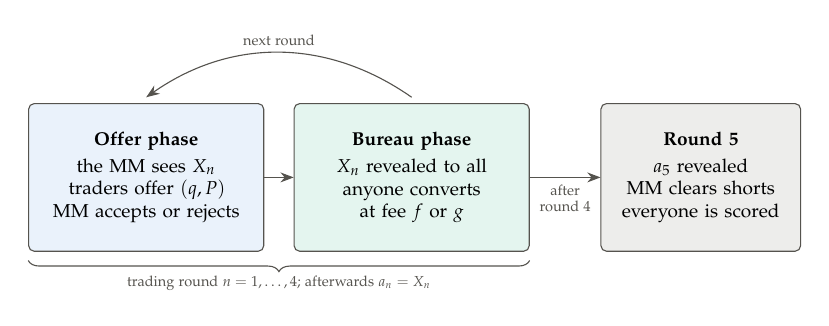
\begin{tikzpicture}[scale=0.75, transform shape, font=\small, >=Stealth,
  phase/.style={draw=cink, rounded corners=2pt, align=center, inner sep=4pt,
                text width=#1, minimum height=25mm, execute at begin node={\hyphenpenalty 10000 }},
  phase/.default=37mm]
  \node[phase, fill=cblue!10] (o) {\textbf{Offer phase}\\[2pt] the MM sees $X_n$\\ traders offer $(q,P)$\\ MM accepts or rejects};
  \node[phase, fill=caqua!12, right=5mm of o] (b) {\textbf{Bureau phase}\\[2pt] $X_n$ revealed to all\\ anyone converts\\ at fee $f$ or $g$};
  \node[phase=31mm, fill=cgrey!25, right=12mm of b] (r5) {\textbf{Round 5}\\[2pt] $a_5$ revealed\\ MM clears shorts\\ everyone is scored};
  \draw[->, cink] (o) -- (b);
  \draw[->, cink] (b) -- node[below, font=\scriptsize, align=center] {after\\ round 4} (r5);
  \draw[cink, decorate, decoration={brace, amplitude=4pt, mirror}]
    ($(o.south west)+(0,-1.5mm)$) -- node[below=4pt, font=\scriptsize] {trading round $n=1,\dots,4$; afterwards $a_n=X_n$} ($(b.south east)+(0,-1.5mm)$);
  \draw[->, cink] ($(b.north)+(0,1mm)$) to[bend right=35] node[above, font=\scriptsize] {next round} ($(o.north)+(0,1mm)$);
\end{tikzpicture}
\caption{One game. The market maker sees each round's rate before the traders' offers; the traders see it only after, when it becomes the anchor for the next round. The Bureau trades at the true rate for a fee.}
\label{fig:timeline}
\end{figure}

\paragraph{Offer phase}
A new exchange rate $X_n$, in dollars per pound, is drawn and shown to the market maker only. The traders, one at a time in an order that changes every round (random in our simulations), may each propose a trade: an amount $q$ of the currency they hold and a price $P$ in dollars per pound. The market maker accepts or rejects each offer on seeing it.

\paragraph{Bureau phase}
The rate $X_n$ is then revealed to everyone and becomes the last known rate $a_n=X_n$. Both the traders and the market maker may convert currency at the Bureau at the rate $a_n$. A trader selling $m$ units receives $(1-f)m$ units' worth of the other currency at that rate, and the market maker pays $g$ in the same way. The rules set $f=\val{p.f}$ and $g=\val{p.g}$; \cref{tab:params} lists every parameter.

In round 5 the rate $a_5$ is drawn and revealed, and the market maker must clear any negative balance at the Bureau at fee $g$. Every trader's position is then scored at $a_5$. Players see the full history of revealed rates, so what a trader knows when it makes its round-$n$ offer is the rate path up to $a_{n-1}$ and its own balances.

\subsection{Exchange-rate dynamics}\label{sec:rate}
The rules generate the rate as an additive random walk,
\begin{equation}\label{eq:walk}
  a_n = a_{n-1} + Z_n,\qquad Z_n\overset{\text{iid}}{\sim}\N(0,\sigma^2),\qquad a_0=\val{p.a0},\quad \sigma=\val{p.sd},
\end{equation}
so a round's move has standard deviation $\sigma/a_0=\val{p.sdrel}$ of the starting rate. This is the discrete-time form of Bachelier's model. The walk is a martingale in dollars per pound: $\E[a_{n+1}\mid a_n]=a_n$. Because the increments are independent, the last revealed rate is a sufficient statistic for the future: optimal play in round $n$ depends on the history only through $a_{n-1}$, the rounds left and the player's balances. The dynamic programme of \cref{sec:exact} uses this state; the networks of \cref{sec:method} are also shown the last few moves, which add nothing to a forecast of the rate, though they may say something about the other agents' positions.

\begin{remark}[Negative rates]\label{rem:negative}
An additive walk can go negative, and a negative exchange rate has no meaning. We delete any simulated path on which a rate reaches zero. At the game's $\sigma=\val{p.sd}$ the chance that any of the five rates is non-positive is below \val{neg.sd05} (\cref{app:parameters}, \cref{tab:negative}), so the deletion changes no number in this paper.
\end{remark}

\subsection{The one-sided martingale}\label{sec:martingale}
The rules score each trader in its starting currency. The rate in pounds per dollar is $1/a_n$, and $x\mapsto 1/x$ is strictly convex.

\begin{proposition}[One-sided martingale]\label{prop:siegel}
Let $(a_n)$ be a positive martingale under a fixed probability measure, with $\E[1/a_n]<\infty$ for every $n$. Then $(1/a_n)$ is a submartingale, $\E[1/a_{n+1}\mid a_n]\ge 1/a_n$, with strict inequality wherever the conditional law of $a_{n+1}$ given $a_n$ is not a point mass. No non-constant positive process and its reciprocal are both martingales under the same measure.
\end{proposition}

\begin{proof}
The map $x\mapsto1/x$ is strictly convex on $(0,\infty)$, so by the conditional Jensen inequality, $\E[1/a_{n+1}\mid a_n]\ge 1/\E[a_{n+1}\mid a_n]=1/a_n$, with equality only where $a_{n+1}$ is almost surely constant given $a_n$. If a positive process and its reciprocal were both martingales, equality would hold at every step, so every increment would be degenerate and the process constant.
\end{proof}

\begin{remark}[Expectations of $1/X$]\label{rem:inverse}
One dollar is worth $1/X$ pounds, so the paper needs $\E[1/X]$. For a Gaussian rate this expectation does not exist: $X$ can land arbitrarily close to $0$, where $1/X$ blows up, and $\int_0 dx/x$ diverges. Deleting negative paths (\cref{rem:negative}) does not fix this, because the trouble comes from rates just above zero. That region is never reached in practice: the starting rate is \val{p.a0sd} standard deviations above zero. We therefore work with the rate law truncated to within 8 standard deviations of the current rate (12 for one blind offer), and every $\E[1/X]$ in the paper is computed under it. The truncation removes probability at most \val{neg.cut8}, so the simulated paths, drawn from the untruncated walk, practically never leave it; but a small removed probability does not by itself bound the change in $\E[1/X]$, which is undefined without the truncation. At every rate the dynamic programme uses, and at $a_0$ for one blind offer, the window lies above zero and is symmetric about the current rate, so the truncated rate is positive with the same mean, has $\E[1/X]<\infty$, and satisfies the assumptions of \cref{prop:siegel}; the untruncated walk does not.
\end{remark}

Write $\kappa(a)=\E[1/a_5\mid a_4=a]$ for the value, in pounds, of one dollar held into settlement, computed by adaptive quadrature over rates within 8 standard deviations (\cref{rem:inverse}). At $a=a_0$, $\kappa=\val{kappa.one}$ against $1/a_0=\val{kappa.recip}$: a dollar held for one more round is worth \val{kappa.onebonus} more in pounds than its current price suggests, and over four rounds the premium is \val{kappa.fourbonus}.

The asymmetry has direct consequences. A pound seller who converts early holds dollars for longer and collects this premium; a dollar seller converting early holds pounds, which are a martingale in dollars and earn nothing. Consider the simplest strategy for the pound seller T1: make no offers and convert everything at the Bureau in one round. Its expected profit or loss, as a share of its capital, is \val{floor.round1} if it converts in round 1, and \val{floor.round2}, \val{floor.round3} and \val{floor.round4} if it waits until round 2, 3 or 4. The loss is mostly the Bureau fee; each round of waiting costs a further \val{floor.perround} bp, because the dollars are held for one round less. \Cref{sec:carry,sec:carry-learned} show the same force deciding who flattens and who carries.

\begin{remark}[Siegel's paradox, and why a different rate model does not remove it]\label{rem:siegel}
This is Siegel's paradox \citep{siegel1972}. Replacing the additive walk with a log-normal rate that is a martingale in dollars per pound does not help: then $\E[1/X_{n+1}\mid X_n]\,X_n=e^{s^2}$ with $s=\sigma/a_0$, a premium of \val{siegel.lnone} per round, the same order as here, and a log-normal rate with zero drift in its logarithm makes \emph{both} currencies drift upwards. In continuous-time finance the resolution is that each currency has its own pricing measure, related by a change of numéraire \citep{geman1995}. In this game every player is told the same rate process, so no such resolution is available: the one-sided martingale is part of the game, and the paper treats it as such.
\end{remark}

\subsection{The traders}\label{sec:traders}
Each trader $i$ starts with $L_i$ units of one currency and a target $T_i$ in the other (\cref{tab:cards}). T1 and T3 hold pounds and want dollars (\emph{pound sellers}); T2 and T4 hold dollars and want pounds (\emph{dollar sellers}). A trader that ends the game holding $c$ units of its starting currency and $d$ units of its target currency pays a residue penalty $\alpha$ on $c$ and a deficit penalty $\beta$ on any shortfall below $T$, valued at the round-5 rate without a fee. Its final wealth in its starting currency is
\begin{equation}\label{eq:terminal}
\begin{aligned}
  W &= c\,(1-\alpha) + \frac{d-\beta\max(T-d,\,0)}{a_5} &&\text{(pound seller)},\\
  W &= c\,(1-\alpha) + \bigl(d-\beta\max(T-d,\,0)\bigr)\,a_5 &&\text{(dollar seller)},
\end{aligned}
\end{equation}
and its profit and loss (P/L) is $(W-L)/L$. We quote P/L in per cent of capital, and differences of P/L, such as a strategy's edge over the Bureau, in basis points (bp) of capital. A basis point is one hundredth of a per cent, so an edge of 1 bp is $0.01\%$ of capital. Basis points are of capital unless we say otherwise; the one-offer analysis of \cref{sec:optimal,sec:breakdown} quotes them per pound offered.

\begin{table}[htb]
\centering\small
\begin{threeparttable}
\caption{The four trader cards. The last column is the target as a share of the start valued at $a_0$.}
\label{tab:cards}
\begin{tabular}{llrrrrr}
\toprule
 & role & start $L$ & target $T$ & residue $\alpha$ & deficit $\beta$ & target / fair value\\
\midrule
\tablebody{tables/tab_cards.tex}
\bottomrule
\end{tabular}
\end{threeparttable}
\end{table}

\subsection{The market maker}\label{sec:mm}
The market maker starts with nothing. It may run negative balances during the game but must end round 5 with none, clearing any short position at the Bureau at fee $g$. Its score is its final surplus in pounds at $a_5$, as a share of all the traders' starting capital at $a_0$, which we call \emph{the game's capital}: \pounds\val{cards.capital} for the four cards, and the one trader's capital in a game with one trader. We quote it in basis points. When it accepts a pound seller's offer at price $P$ it buys pounds and owes dollars; it can hedge immediately at the Bureau (\emph{flatten}), hold the position to a later round, at the latest the forced clear in round 5 (\emph{carry}), or offset it against a dollar seller's trade (\emph{net}).

\subsection{Modelling choices}\label{sec:assumptions}
The model follows the rules, with four choices. First, each trader makes one offer per round. The rules put no limit on offers inside the three-minute window, but with unlimited offers a trader facing an informed market maker can bisect its way to the rate; the value of repeated offers is answered briefly in \cref{app:sequential}, and the results of \cref{sec:exact,sec:fee} are conditional on one offer per round. Second, every agent knows the rate's step distribution, so $\sigma$ is known and fixed; the networks are not given $\sigma$ as an input but are trained and tested at that $\sigma$, and uncertainty about $\sigma$ is left to future work. Third, every agent is risk neutral and maximises its expected score. Fourth, traders may offer to the market maker in either direction (\emph{two-way} trading) and may convert any fraction of their starting currency at the Bureau, but only towards their target, never back. This is a modelling restriction: converting back pays the fee twice, and we do not prove that it is never useful once the penalties are taken into account.

%%% ---- sections/s4_exact ----
% =============================================================================
\section{Exact analysis of the single-trader problem}\label{sec:exact}
% =============================================================================
This section solves the trader's problem for one trader facing a market maker that accepts any offer better for it than the true rate. One blind offer is solved in closed form (\cref{sec:oneshot,sec:optimal}); the full four-round card game is solved by dynamic programming, which is exact in principle and here is computed on grids whose error we measure (\cref{sec:multiround,sec:bias}). The market maker's own Bureau fee is set to zero here. This is not a loss of generality: \cref{sec:fee} adds the fee and shows that, against a market maker that hedges each fill at once, the game with it is exactly a rescaled version of the game without it (\cref{prop:card}), so every result of this section carries over.

\subsection{One blind offer}\label{sec:oneshot}
Take a pound seller with one unit to sell, one round and one offer. The round's rate is $X\sim\N(a_0,\sigma^2)$, unseen. The trader offers price $P$; the market maker accepts if and only if $P<X$, and a rejected trader converts at the Bureau at $(1-f)X$. Call the expected dollars per pound from offering at $P$ the \emph{offer value} $G(P)$:
\begin{equation}\label{eq:G}
  G(P) \;=\; \underbrace{P\,\Pr(X>P)}_{\text{accepted}} \;+\; \underbrace{(1-f)\,\E\big[X\,\1\{X\le P\}\big]}_{\text{rejected: Bureau at the revealed rate}}.
\end{equation}

With $z_P=(P-a_0)/\sigma$ and the standard normal distribution and density $\Phi,\varphi$, the Gaussian identity $\E[X\1\{X\le P\}]=a_0\Phi(z_P)-\sigma\varphi(z_P)$ gives
\begin{equation}\label{eq:Gclosed}
  G(P) = P\,\big(1-\Phi(z_P)\big) + (1-f)\,\big(a_0\Phi(z_P)-\sigma\varphi(z_P)\big).
\end{equation}
Offering nothing is worth the \emph{Bureau floor} $(1-f)a_0=\val{v0.floor}$ dollars per pound. Knowing $X$ in advance would be worth $a_0$. The fee $fa_0=\val{v0.pie}$ dollars per pound is therefore the whole prize the offer can win back.

\subsection{The optimal offer and adverse selection}\label{sec:optimal}
Differentiating \eqref{eq:Gclosed}, with $dz_P/dP=1/\sigma$ and $\varphi'(z)=-z\varphi(z)$, gives
\[
G'(P) = \big(1-\Phi(z_P)\big) - \frac{P}{\sigma}\varphi(z_P) + (1-f)\Big(\frac{a_0}{\sigma}+z_P\Big)\varphi(z_P).
\]
Since $a_0/\sigma+z_P=P/\sigma$, the $\varphi$ terms from the two branches cancel except for the fee:
\begin{equation}\label{eq:Gprime}
  G'(P) = \big(1-\Phi(z_P)\big) - \frac{fP}{\sigma}\,\varphi(z_P).
\end{equation}

\begin{proposition}[Optimal blind offer]\label{prop:foc}
For $f>0$ the offer value has a unique maximum, at the price where the probability of a fill equals the marginal cost of asking more,
\begin{equation}\label{eq:foc}
  1-\Phi(z_{P^*}) = \frac{fP^*}{\sigma}\,\varphi(z_{P^*}).
\end{equation}
\end{proposition}

\begin{proof}
With $z=z_P$ and $fP/\sigma=fa_0/\sigma+fz$, write \eqref{eq:Gprime} as
\[
G'(P)=\varphi(z)\Big[m(z)-\frac{fa_0}{\sigma}-fz\Big],\qquad m(z)=\frac{1-\Phi(z)}{\varphi(z)},
\]
where $m$ is the Mills ratio of the normal distribution, which is strictly decreasing, tends to $+\infty$ as $z\to-\infty$ and behaves like $1/z$ as $z\to\infty$. The term $fa_0/\sigma+fz$ is strictly increasing in $z$. The bracket is therefore positive for small $z$, negative for large $z$, and changes sign exactly once. So $G$ increases up to a single price and decreases after it, and that price is the unique maximum, where \eqref{eq:foc} holds.
\end{proof}

Since $G$ falls back to the floor as $P\to\infty$, its maximum lies above the floor: for the pound seller a blind offer is always worth making, and the question is how much. At the game's parameters, solving \eqref{eq:foc} by Brent's method \citep{brent1973}, the optimal offer is $P^*=\val{v0.Pstar}$, which is $\val{v0.zstarfine}\,\sigma$ above the anchor. It fills with probability \val{v0.fillfine} and is worth $G(P^*)=\val{v0.value}$, against the floor of \val{v0.floor}: the best blind offer wins back \val{v0.share} of the fee. The dollar seller is not the mirror image. It receives $1/P$ pounds per dollar, a convex function of the price, and its best offer is $1/P=\val{v0B.offer}$ pounds per dollar, $\val{v0B.zstar}\,\sigma$ below the anchor in dollars per pound. That offer fills \val{v0B.fill} of the time and wins back \val{v0B.share} of its fee (\cref{fig:oneshot}).

\begin{figure}[H]
\centering
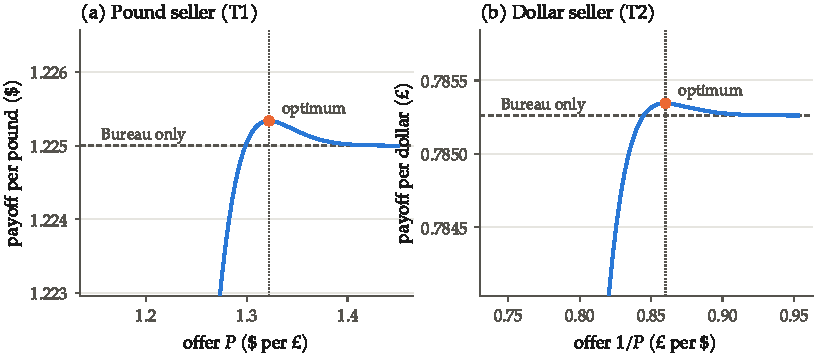
\includegraphics[width=0.9\textwidth]{figures/fig_oneshot}
\caption{The value of one blind offer for (a) the pound seller and (b) the dollar seller, against the Bureau-only floor (dashed). The maximum is shallow: the whole prize is the Bureau fee, and a blind offer wins back \val{v0.share} of it for the pound seller and \val{v0B.share} for the dollar seller. Parameters: $a_0=\val{p.a0}$, $\sigma=\val{p.sd}$, $f=\val{p.f}$, no market-maker fee.}
\label{fig:oneshot}
\end{figure}

Why so little? A fill happens only when $X>P$, and it beats the Bureau only when $P>(1-f)X$. The offer makes money only in the band
\begin{equation}\label{eq:band}
  (1-f)X < P < X,
\end{equation}
and loses money relative to the Bureau whenever the rate has risen further. This is adverse selection in its simplest form, the Glosten--Milgrom argument with the roles reversed: the market maker's acceptance tells the trader that it has sold too cheaply.

The size of the offer is not a real choice.

\begin{lemma}[All or nothing]\label{lem:aon}
If the trader offers a fraction $q\in[0,1]$ of its holding at price $P$ and converts the rest at the Bureau, its expected payoff is $q\,G(P)+(1-q)(1-f)a_0$, linear in $q$. The optimum is at $q=1$ whenever an offer is worth making.
\end{lemma}


%\begin{proof}
%The offered part earns $G(P)$ per unit and the rest is converted at the Bureau at the revealed rate, worth $(1-f)a_0$ per unit in %expectation, so the payoff is linear in $q$ and maximised at an end point.
%\end{proof}

\begin{proof}
The payoff is affine in $q$: it equals $(1-f)a_0+q\,[G(P)-(1-f)a_0]$. It is therefore maximised at $q=1$ when $G(P)>(1-f)a_0$, at $q=0$ when $G(P)<(1-f)a_0$, and by every $q$ when the two are equal.
\end{proof}

\paragraph{Valuation currency}
The one-offer analysis here and in \cref{sec:rho,sec:breakdown} values each side in its target currency, dollars for the pound seller and pounds for the dollar seller, which is what gives the closed form. The rules score each trader in its starting currency. Scored in pounds at the revealed rate, the pound seller's best offer moves by $\val{num.dz}\,\sigma$, to $P=\val{num.Pstar}$; it fills \val{num.fill} of the time and beats the Bureau by \val{num.edgebp} bp of the pound offered, against \val{num.edgedbp} bp valued in dollars. The difference is the premium of \cref{prop:siegel}; we have not redone the dollar seller's one-offer analysis in its scoring currency. The dynamic programme of \cref{sec:multiround}, and every value in \cref{tab:feedp}, uses the rules' scoring.

\subsection{The multi-round problem}\label{sec:multiround}
The full card game adds four rounds, sized offers, the option to carry currency between rounds, and the penalties of \eqref{eq:terminal}. The trader's state entering round $n$ is its holding $c$ of starting currency, its holding $d$ of target currency and the anchor $a=a_{n-1}$. Let $W_n(c,d,a)$ be the best expected final wealth from that state; it satisfies Bellman's recursion \citep{bellman1957}. At settlement, for a pound seller,
\begin{equation}\label{eq:W5}
  W_5(c,d,a_4) = c\,(1-\alpha) + \big[d-\beta\max(T-d,\,0)\big]\,\kappa(a_4),
\end{equation}
and each round solves two nested problems backwards. After the rate $X$ is revealed the trader chooses how much to convert at the BdC, $m\in[0,c]$:
\begin{equation}\label{eq:bureaustage}
  R_n(c,d,X) = \max_{0\le m\le c} W_{n+1}\big(c-m,\; d+(1-f)Xm,\; X\big).
\end{equation}
Before it, with one offer of size $q$ at price $P$, sent to the market maker and accepted with probability $1-\Phi(z_P)$ where $z_P=(P-a)/\sigma$,
\begin{equation}\label{eq:bellman}
\begin{aligned}
  W_n(c,d,a) = \max_{P,\,q}\; \E_X\Big[\,&\1\{X>P\}\,R_n(c-q,\,d+Pq,\,X)\\
  {}+{}&\1\{X\le P\}\,R_n(c,\,d,\,X)\Big],
\end{aligned}
\end{equation}
Offers sell the trader's starting currency only, so this benchmark omits the reverse offers that \cref{sec:assumptions} allows; the learning experiments of \cref{sec:results} allow them, and no trader uses them (\cref{sec:four}). The recursion is solved on grids for $(c,d,a)$, the price and the rate, described in \cref{app:numerics}. For a dollar seller an accepted offer adds $q/P$ pounds, the Bureau pays $(1-f)m/X$, and the settlement value of target currency is linear, $\E[a_5\mid a_4]=a_4$, in place of $\kappa(a_4)$ in \eqref{eq:W5}.

With one offer per round, T1's optimal play has an expected P/L of \val{dp.A.f2g0.value}, against \val{dp.A.f2g0.floor} for converting everything at the Bureau in round 1 (the \emph{Bureau floor}), an edge of $\val{dp.A.f2g0.edge}\pm\val{dp.A.f2g0.edgese}$ bp. For T2 the corresponding numbers are \val{dp.B.f2g0.value} against \val{dp.B.f2g0.floor}, an edge of $\val{dp.B.f2g0.edge}\pm\val{dp.B.f2g0.edgese}$ bp. These values come from replaying the optimal policy on 200{,}000 simulated games (\cref{sec:bias} explains why). The edge compares the whole policy with converting everything in round 1, so it includes any gain from the timing and size of Bureau conversions as well as from offers.

\subsection{Currency asymmetry in optimal play}\label{sec:carry}
The two sides play differently. T1 makes one offer in round 1, $\val{dp.A.f2g0.r1z}\,\sigma$ above the anchor, which fills \val{dp.A.f2g0.r1fill} of the time; it then converts everything left at the Bureau in the same round (\val{dp.A.f2g0.bdc1} of its capital) and carries nothing. T2 offers every round and spreads its Bureau conversions: \val{dp.B.f2g0.bdc1} of its capital in round 1, then \val{dp.B.f2g0.bdc2}, \val{dp.B.f2g0.bdc3} and \val{dp.B.f2g0.bdc4} (\cref{fig:flows}).

\begin{figure}[htb]
\centering
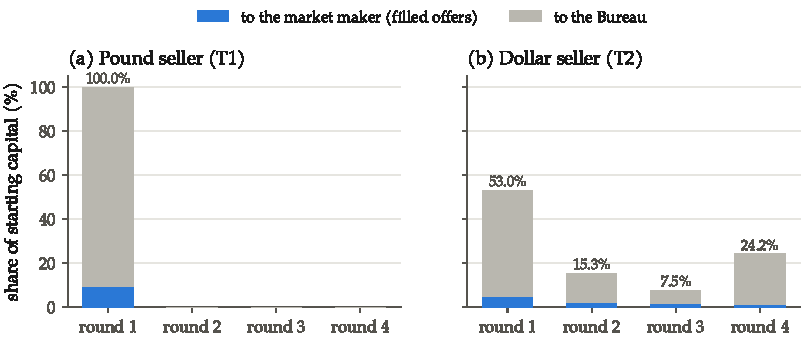
\includegraphics[width=0.9\textwidth]{figures/fig_flows}
\caption{Where the optimal policy sends each trader's capital, round by round, at $(f,g)=(\val{p.f},0)$: to the market maker through filled offers, or to the Bureau. (a) The pound seller T1 converts everything in round 1. (b) The dollar seller T2 offers every round and spreads its conversions. Shares of starting capital, from the dynamic programme's policy replayed on 200{,}000 games; bar labels are each round's total.}
\label{fig:flows}
\end{figure}

\Cref{prop:siegel} explains the difference. A pound seller that converts in round 1 holds dollars through four rate steps and collects the premium of \cref{sec:martingale}; as shown there, each round it waits costs it \val{floor.perround} bp on average, far more than another blind offer can earn. A dollar seller that converts holds pounds, which earn no premium in dollars. For T2, the simplest strategy of \cref{sec:martingale}, making no offers and converting everything at the Bureau in one round, has an expected P/L of \val{floorB.round1} in round 1 and \val{floorB.round4} in round 4: waiting costs only \val{floorB.perround} bp per round, through the kink of its deficit penalty, and keeps the option of another offer.

\subsection{Value and policy}\label{sec:consistency}
A dynamic programme produces two things: the optimal value, read from its table, and the optimal policy. The policy can be put back into the game and played through the rules, which is a check of both. We apply five checks (\cref{app:verification}): the one-round problem must reproduce the closed form of \cref{sec:optimal}; the market maker's fee must reproduce \cref{prop:card} below; the replayed policy must return the table value; money must be conserved between the three parties on every path; and the value must lie between the Bureau floor and the value of perfect foresight.

\begin{remark}[The value of information]\label{rem:clairvoyant}
A trader who knew the whole rate path would sell to the market maker in the round with the best rate, at that rate, choosing how much to sell given its card. Its expected P/L is \val{dp.A.f2g0.cv} for T1 and \val{dp.B.f2g0.cv} for T2, against \val{dp.A.f2g0.value} and \val{dp.B.f2g0.value} for optimal play. Most of what separates a trader from a perfect score is information it does not have.
\end{remark}

\subsection{Numerical accuracy of the table value}\label{sec:bias}
The third check exposes a numerical bias. On 200{,}000 paths, T1's table value exceeds its replayed value by \val{dp.A.f2g0.gapfa} bp, while for T2 the gap is \val{dp.B.f2g0.gapfa} bp. The table stores the value function only at grid points of the anchor and interpolates linearly between them. T1's value depends on the anchor through $\kappa$, which is convex, and a straight line between two grid points of a convex function lies above the curve, so interpolation overstates it (\cref{fig:interp}); T2's settlement is linear in $a_5$ and shows no such bias.

\begin{figure}[htb]
\centering
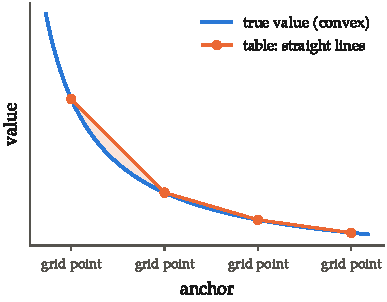
\includegraphics[width=0.55\textwidth]{figures/fig_interp}
\caption{Why the table value is biased for the pound seller (schematic, curvature exaggerated). For a value that is convex in the anchor, the table holds it at grid points and joins them with straight lines, which lie above the curve. The shaded gap is the overstatement.}
\label{fig:interp}
\end{figure}
 In a separate refinement on 20{,}000 paths (\cref{app:numerics}), halving the anchor step twice takes T1's gap from \val{refine.gap13} to \val{refine.gap25} and then \val{refine.gap49} bp, falling by factors of \val{refine.ratioa} and \val{refine.ratiob}, while the replayed value stays at \val{refine.replay13}. The policy does not change: replayed on the same 20{,}000 paths, the policy from the finest anchor grid gives the same final wealth as the default grid's on \val{gridchk.anchor.same} path. Holdings grids twice as fine leave T1's policy unchanged too, and change T2's value by $\val{gridchk.cdB.diff}\pm\val{gridchk.cdB.diffse}$ bp (\cref{app:numerics}). What is biased is the table's own estimate of the value. Every DP value quoted in this paper is therefore taken from Monte Carlo simulation rather than from the table: the optimal policy is played through the rules on simulated paths, and its value is reported as the Bureau floor, computed by quadrature, plus the average paired difference between the policy and the Bureau on those paths. A replayed value is the value of a policy the dynamic programme found, so, up to Monte Carlo error, it is a lower bound on the best possible value; \cref{app:numerics} bounds part of what the grids leave out.

%%% ---- sections/s5_fee ----
% =============================================================================
\section{The market maker's fee and the breakdown of trade}\label{sec:fee}
% =============================================================================
So far the market maker accepted any offer better than the true rate. In the game it pays a fee $g=\val{p.g}$ whenever it converts at the Bureau, and a rational market maker prices that in. This section derives the acceptance rule that follows, shows that the game with this fee reduces exactly to the game of \cref{sec:exact}, and uses that reduction to explain why the offer channel is almost worthless at the rules' fees.

\subsection{The fee-adjusted acceptance rule}\label{sec:rule}
A market maker that fills an offer takes on a position in one currency. To \emph{flatten} it is to convert that position back at the Bureau in the same round, so that it holds no exposure to later moves of the rate. We take the market maker to accept an offer only if the fill is profitable after flattening, and call this the \emph{flatten rule}. We use it as the benchmark because it is the market maker's best choice fill by fill against a pound seller, and because a flattened fill leaves no position behind, so the verdict depends only on the round's rate, not on the market maker's book or on later rounds. Against a dollar seller carrying would do better (\cref{rem:carrymm}). We did not re-solve the dynamic programme for a market maker that carries, but the learned market makers of \cref{sec:results} are free to carry, and against a dollar seller they do (\cref{sec:carry-learned}).

\medskip
Suppose a pound seller offers $q$ pounds at $P$ dollars per pound and the round's rate is $X$. If the market maker fills, it pays $Pq$ dollars and receives $q$ pounds. Flattening sells the $q$ pounds at the Bureau for $(1-g)Xq$ dollars. Its profit is
\[
  q\,\big[(1-g)X - P\big],
\]
which is positive exactly when $P<(1-g)X$. Suppose instead a dollar seller offers $D$ dollars at $P$. The market maker receives $D$ dollars and pays $D/P$ pounds; flattening sells the dollars for $(1-g)D/X$ pounds, a profit of $D\big[(1-g)/X-1/P\big]$, positive exactly when $P>X/(1-g)$.

Either way the verdict depends on the rate only through one threshold. A pound seller's offer at $P$ is filled if and only if
\[
  X > x^* = \frac{P}{1-g}.
\]
Choosing the offer $P$ is the same as choosing the threshold $x^*=P/(1-g)$, so from now on we describe each offer by its threshold. An acceptance still tells the trader only that $X$ is above it.

\begin{remark}[A market maker that carries]\label{rem:carrymm}
Against a pound seller the flatten rule is the market maker's best choice fill by fill: the fill leaves it short dollars, and carrying them to round 5 costs it the premium of \cref{prop:siegel}. Against a dollar seller it is not: the fill leaves it long dollars and carrying earns the premium, so it would accept offers that ask for more pounds per dollar. At the rules' fees, the dollar seller's best single offer wins back \val{carrymm.f2g1.carryshare} of its fee against a market maker that carries, and \val{carrymm.f2g1.flatshare} against one that flattens: far more, but still almost nothing, so a single offer stays almost worthless either way.

\medskip
These figures come from the one-offer calculation of \cref{sec:optimal}, with the carrying market maker accepting when $1/P<(1-g)\,\E[1/a_5\mid a_1=X]$ instead of $1/P<(1-g)/X$.
\end{remark}

\subsection{An equivalent game without the market maker's fee}\label{sec:card}
The idea is simple. The market maker's fee only scales the price at which it accepts by $(1-g)$, and counting dollars in units of $(1-g)$ undoes that scaling. What is left is how much more the trader pays the Bureau than the market maker does, a fee $\fp\approx f-g$. So the game with both fees is the game of \cref{sec:exact} with one smaller trader fee, and everything there carries over.
\medskip

Take a pound seller; the dollar seller is the mirror image, worked through in the proof of \cref{prop:card}.Write \emph{the $g=0$ game} for the game of \cref{sec:exact}: the market maker pays no Bureau fee and accepts when $X>P$, and the trader still pays $f$. In the game with the fee, a fill at threshold $x^*$ pays the trader $P=(1-g)x^*$ dollars per pound, and a Bureau conversion pays $(1-f)X$. Count dollars in units of $(1-g)$, that is, divide both payments by $(1-g)$:
\begin{align*}
  \text{fill:}\quad & \frac{(1-g)\,x^*}{1-g} = x^*,\\
  \text{Bureau:}\quad & \frac{(1-f)\,X}{1-g} = \Big(1-\frac{f-g}{1-g}\Big)X = (1-\fp)\,X,
\end{align*}
where the middle step uses $1-f=(1-g)-(f-g)$, and
\begin{equation}\label{eq:fprime}
  \fp = \frac{f-g}{1-g}.
\end{equation}
The fill now pays exactly what an offer at $x^*$ pays in the $g=0$ game, where the market maker accepts when $X>x^*$, and the Bureau pays what it pays in the $g=0$ game with trader fee $\fp$.
In words, $\fp$ is the trader's Bureau fee measured against the market maker's: for every dollar the market maker would get from the Bureau, the trader gets $1-\fp$. It is the part of the trader's fee that a fill can still save, and is close to $f-g$. The same rescaling applies to the card, which gives the following result.

\begin{proposition}[Equivalent game without the market maker's fee]\label{prop:card}
Let $V^{f,g}(T,\alpha,\beta)$ be the optimal expected final wealth of a trader with target $T$ and penalties $\alpha,\beta$, with trader BdC fee $f$ and market-maker BdC fee $g<f$, against a market maker that accepts exactly the offers it can flatten at a profit. For any number of rounds and any number of sized offers per round in the trader's own direction,
\begin{equation}\label{eq:card}
  V^{f,g}(T,\alpha,\beta) \;=\; (1-g)\,V^{\fp,0}\!\left(\frac{T}{1-g},\; 1-\frac{1-\alpha}{1-g},\; \beta\right),
\end{equation}
and the optimal thresholds of the two games coincide.
\end{proposition}

\begin{proof}
Consider a pound seller. A policy chooses, at each offer, a size $q$ and a price, and at each Bureau phase an amount $m$, all as functions of the history. At $(f,g)$ an offer at price $P$ is filled exactly when $X>P/(1-g)$; in the $g=0$ game an offer at price $P'$ is filled exactly when $X>P'$. Describing every offer by its threshold $x^*$, with $P=(1-g)x^*$ in the first game and $P'=x^*$ in the second, puts the policies of the two games in one-to-one correspondence, and corresponding policies are filled on the same paths. So the history (revealed rates and fills), and hence every action, is the same in both games.

At $(f,g)$ a fill adds $q(1-g)x^*$ dollars and a conversion adds $m(1-f)X$. Count dollars in units of $(1-g)$, $\tilde d=d/(1-g)$: a fill then adds $qx^*$ and a conversion $m(1-\fp)X$, which are the transitions of the $g=0$ game with trader fee $\fp$. Pounds are not rescaled, so the same $q$ and $m$ are feasible in both games. At settlement, with $\tilde T=T/(1-g)$ and $1-\tilde\alpha=(1-\alpha)/(1-g)$, and since $\max(T-d,0)=(1-g)\max(\tilde T-\tilde d,0)$,
\[
c(1-\alpha)+\frac{d-\beta\max(T-d,0)}{a_5} = (1-g)\left[c\,(1-\tilde\alpha)+\frac{\tilde d-\beta\max(\tilde T-\tilde d,0)}{a_5}\right].
\]
So on every path, every policy's final wealth at $(f,g)$ is $(1-g)$ times the final wealth of the corresponding policy in the $g=0$ game with trader fee $\fp$, on the card $(\tilde T,\tilde\alpha,\beta)$. Taking expectations, with the convention of \cref{rem:inverse}, and maximising over corresponding policies gives \eqref{eq:card}. Since $1-g>0$, a policy is optimal in one game exactly when the corresponding policy is optimal in the other, so the optimal thresholds coincide.

For a dollar seller the argument is the same with pounds counted in units of $(1-g)$, except that the market maker fills when $X<(1-g)P$, so the threshold is $x^*=(1-g)P$, and settlement uses $a_5$ in place of $1/a_5$.
\end{proof}

\Cref{prop:card} is a change of units, not a new mechanism, but it is what lets one family of solutions cover every fee pair. In the dynamic programme the two sides of \eqref{eq:card} agree in every table to within \val{gate2.game} of capital. The rescaled residue penalty $\tilde\alpha=(\alpha-g)/(1-g)$ is negative when $\alpha<g$, a small reward for leftover currency; the identity still holds, because it holds path by path for every policy. With one round there is no card, and the proposition reduces to a statement about the single offer of \cref{sec:oneshot}.

\begin{corollary}[One round]\label{cor:oneround}
With one round, the game with fees $(f,g)$ is the $g=0$ game with trader fee $\fp$, scaled by $(1-g)$: the optimal threshold solves \eqref{eq:foc} with $\fp$ in place of $f$.
\end{corollary}

\begin{proof}
Counting the payoff in target currency, the argument above gives $G^{f,g}(x^*)=(1-g)\,G^{\fp,0}(x^*)$ for every threshold $x^*$.
\end{proof}

\subsection{The governing ratio}\label{sec:rho}
Two things follow. What matters is $\fp\approx f-g$, not $f$; and it matters relative to a step of the rate. By \cref{cor:oneround}, the best threshold $x^*$ solves \eqref{eq:foc} with $\fp$ in place of $f$:
\[
1-\Phi(z)=\frac{\fp x^*}{\sigma}\,\varphi(z),\qquad z=\frac{x^*-a_0}{\sigma}.
\]
Writing the threshold as $x^*=a_0+\sigma z$ splits the right-hand side into a part that does not depend on $z$ and a small part that does,
\[
\frac{\fp x^*}{\sigma}=\frac{\fp(a_0+\sigma z)}{\sigma}=\frac{\fp a_0}{\sigma}+\fp z,
\]
so the optimal $z$ solves
\begin{equation}\label{eq:rhofoc}
  1-\Phi(z) = (\rho+\fp z)\,\varphi(z),\qquad \rho = \frac{\fp a_0}{\sigma}.
\end{equation}
Since $\fp z$ is smaller than $\rho$, the threshold in units of $\sigma$ is set, to leading order, by $\rho$ alone. We call $\rho$ the \emph{governing ratio}: the fee a fill can save, as a multiple of one step of the rate. Without a market-maker fee the game has $\rho=\val{fee.rho20}$; at the rules' fees, $\rho=\val{fee.rho21}$.

To read it: a fill can save at most $\fp=\val{fee.fprime21}$ of the rate, while the rate moves by $\sigma/a_0=\val{p.sdrel}$ of itself in a round, so at the rules' fees the saving is about a quarter of one step. \Cref{fig:strips} shows what this means. A fill beats the Bureau only if the rate lands in a window just above the threshold, of width about $\fp x^*\approx\rho\sigma$; if the rate lands above that window, the fill loses to the Bureau. When $\rho$ is large the window is wide beside the rate's spread, and an offer near the anchor fills mostly inside it (\cref{fig:strips}a, $\rho=\val{fee.rho20}$). When $\rho$ is small the window is a sliver, and the best offer moves so far out that it almost never fills (\cref{fig:strips}c, $\rho=\val{fee.rho21}$).

\subsection{Breakdown of the offer channel}\label{sec:breakdown}
At the rules' fees, $f=\val{p.f}$ and $g=\val{p.g}$, the pound seller's best threshold is $\val{fee.z21}\,\sigma$ above the anchor, and it fills \val{fee.fill21} of the time. It beats the Bureau by \val{fee.edge21bp} bp of the value of the pound offered, \val{fee.share21} of the most it could win, the gap $(f-g)a_0$ between the floor and perfect information (with $g=0$ this gap is the fee $fa_0$ of \cref{sec:oneshot}). The dollar seller's best threshold is $\val{fee.Bz21}\,\sigma$ below the anchor and fills \val{fee.Bfill21} of the time. We say the offer channel has \emph{broken down} when the policy the dynamic programme finds is worth less than one basis point of capital more than the Bureau. Its replayed value is the value of an actual policy, so it is a lower bound on what the trader can achieve; we have no matching upper bound (\cref{app:numerics}). Breakdown is also a matter of degree: without the market maker's fee the pound seller's computed policy gains only \val{dp.A.f2g0.edgebp} bp of capital over the Bureau floor (\cref{tab:feedp}), so the line between open and broken is a few basis points.

\Cref{fig:strips} shows why, in terms of where the round's rate lands: a filled offer beats the Bureau when the rate lands in the green region just above the threshold, and loses to it when the rate lands further up, in the red. At the optimum of the $g=0$ game, $P=\val{v0.Pstar}$, green fills happen in \val{strip.beatsg0} of rounds and red ones in \val{strip.worseg0} (panel a). A market-maker fee of \val{p.g} raises the acceptance threshold to $P/(1-g)$, which removes most of the green and none of the red: green falls to \val{strip.beatsg1}, red stays at \val{strip.worseg1}, and the offer now loses more often than it wins (panel b). The trader's answer is to move its offer out until the green again outweighs the red (panel c). That works because far out in the normal tail the density falls so steeply that a rate past the threshold is usually only just past it, so the red shrinks faster than the green; but it happens only about $\val{fee.z21}\,\sigma$ out, where the offer is almost never filled.

\begin{figure}[htb]
\centering
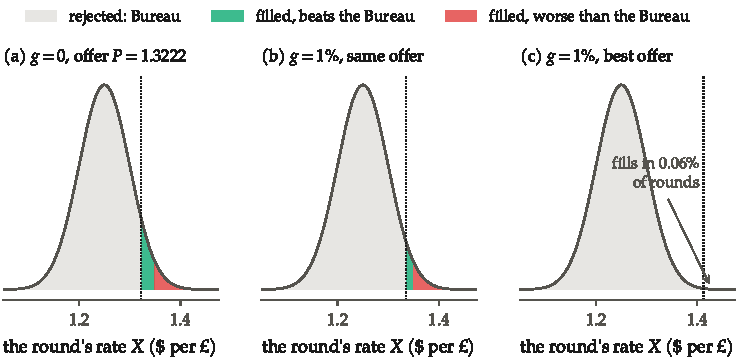
\includegraphics[width=0.95\textwidth]{figures/fig_strips}
\caption{Where a pound seller's offer ends up, over the distribution of the round's rate. The dotted line is the rate above which the market maker accepts. A filled offer beats the Bureau when the rate is below $P/(1-f)$, so the fill pays more than converting would have, and is worse than the Bureau above it. (a) The optimum of the $g=0$ game, $P=\val{v0.Pstar}$, with no market-maker fee ($\rho=\val{fee.rho20}$). (b) The same offer when the market maker pays $g=\val{p.g}$ and accepts only above $P/(1-g)$. (c) The best offer at $g=\val{p.g}$ ($\rho=\val{fee.rho21}$): accepted only above $\val{fee.z21}\,\sigma$ from the anchor, it fills in \val{fee.fill21} of rounds. Parameters: $a_0=\val{p.a0}$, $\sigma=\val{p.sd}$, $f=\val{p.f}$.}
\label{fig:strips}
\end{figure}

What closes the channel is the size of the fee the trader can save relative to a step of the rate, not the market maker's fee as such (\cref{fig:rho}). The collapse is steep: at $\rho=0.5$ the best offer fills \val{rho.filla} of the time and wins back \val{rho.sharea} of the fee, at $\rho=0.35$ it fills \val{rho.fillb}, and at the rules' $\rho=\val{fee.rho21}$ only \val{fee.fill21}, winning back \val{fee.share21}. Anything that raises $\rho$ reopens it. A wider spread does: $(3\%,1\%)$ gives $\fp=\val{fee.fprime31}$ and $\rho=\val{fee.rho31}$, almost exactly the $(2\%,0)$ game, with a threshold $\val{fee.z31}\,\sigma$ out that fills \val{fee.fill31} of the time. So does lower volatility: halving $\sigma$ at the rules' fees doubles $\rho$ and restores a fill probability of \val{fee.fillhalfsd}.

\begin{figure}[htb]
\centering
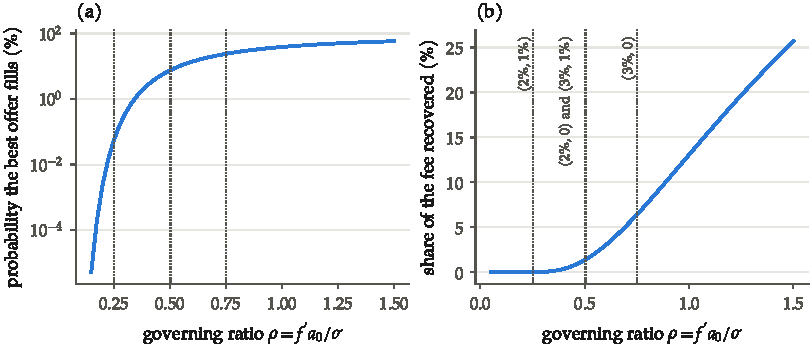
\includegraphics[width=0.9\textwidth]{figures/fig_rho}
\caption{(a) The fill probability and (b) the value of the best blind offer as functions of the governing ratio $\rho=\fp a_0/\sigma$, computed in the $g=0$ game with trader fee $\fp$ and $\sigma=\val{p.sd}$. By \cref{cor:oneround} every fee pair with the same $\fp$ gives the same offer; other volatilities shift the curve only through the small term $\fp z$ in \eqref{eq:rhofoc}. The dotted lines mark the four fee pairs used in this paper.}
\label{fig:rho}
\end{figure}

\subsection{The full game with the fee}\label{sec:fullfee}
By \cref{prop:card}, the game at $(3\%,1\%)$ is not a new game: it is the game at $(\val{fee.fprime31},0)$, almost exactly $(2\%,0)$, with the target raised by \val{card.Tup} and the residue penalty cut, from 2\% to \val{card.alphaA} for T1 and from 3\% to \val{card.alphaB} for T2. \Cref{prop:card} predicts that $(3\%,1\%)$ is nearer $(2\%,0)$ than $(3\%,0)$, and \cref{cor:oneround} that one offer at $(2\%,1\%)$ is almost worthless. \Cref{tab:feedp} solves the full four-round game with one offer per round at the four fee pairs; its last two columns are the trained networks of \cref{sec:validation}.

\begin{table}[htb]
\centering\footnotesize\setlength{\tabcolsep}{4pt}
\begin{threeparttable}
\caption{The full four-round game with one offer per round, against the flatten rule, at four pairs of trader fee $f$ and market-maker fee $g$: the dynamic programme (DP) and the trained single-trader network (\cref{sec:validation}). Bureau floor and DP value are expected P/L; edges over the floor and the DP's lead over the network are in bp of capital, $\pm$ two standard errors of the paired difference on 200{,}000 common paths. Rows are ordered by the fee spread $f-g$: the two pairs with a 2\% spread have nearly the same edge (\cref{prop:card}), although their floors and values differ, because at $(3\%,1\%)$ the trader pays a higher Bureau fee whatever it does.}
\label{tab:feedp}
\begin{tabular}{lcccccc}
\toprule
$(f,g)$ & $f-g$ & Bureau floor & DP value & DP edge & network edge & DP $-$ network\\
\midrule
\tablebody{tables/tab_feedp.tex}
\bottomrule
\end{tabular}
\end{threeparttable}
\end{table}

At $(2\%,1\%)$ neither trader's edge exceeds \val{dp.B.f2g1.hibp} bp of capital even after adding two standard errors, so the offer channel has broken down in the sense of \cref{sec:breakdown}. T2's best single offer at these fees lies $\val{fee.Bz21}\,\sigma$ out, beyond the programme's threshold grid of $\pm4\sigma$, but offers outside the grid could add at most \val{grid.offbound} bp (\cref{app:numerics}). At $(3\%,1\%)$ the edges are those of $(2\%,0)$ to within noise, not those of $(3\%,0)$, and T1's first offer and flows are the same as at $(2\%,0)$.

These results assume one offer per round. With several offers per round a trader can probe the market maker and the conclusion changes (\cref{app:sequential}).

\subsection{Why traders on both sides could still trade}\label{sec:gains}
The breakdown above is a single-trader result. With traders on both sides, the market maker can avoid the adverse selection that causes it, which is why the rest of the paper studies that market.

\begin{remark}[Internalised flow carries no adverse selection]\label{rem:matched}
Suppose a pound seller quotes $P_A$ and a dollar seller $P_B>P_A$ for the same $L$ pounds in the same round; we say such quotes \emph{cross}. If the market maker fills both, its pounds net to zero, it never visits the Bureau, and it is left with $L(P_B-P_A)$ dollars, a gain whatever the rate. Crossing quotes are profitable to fill without any information about $X$: the adverse selection of the one-trader game comes from the market maker's option to fill one side alone.
\end{remark}

\subsection{Hypotheses for the learning experiments}\label{sec:hypotheses}
The results of this section and \cref{sec:exact} suggest five hypotheses for the markets studied with learning agents in \cref{sec:results}. Each follows from a result above; \cref{sec:results} tests them.
\begin{hypothesis}\label{h:threshold}A learned market maker facing one trader recovers the fee-adjusted threshold rule of \cref{sec:rule}.\end{hypothesis}
\noindent The rule accepts exactly the offers that are profitable after flattening (\cref{sec:rule}), and against a pound seller flattening beats carrying fill by fill (\cref{rem:carrymm}), so a market maker that learns well should find it.
\begin{hypothesis}\label{h:cotrain}When one trader and one market maker learn together, trade breaks down at $(2\%,1\%)$ but not at $(3\%,1\%)$ or $(2\%,0)$.\end{hypothesis}

\begin{hypothesis}\label{h:net}With traders on both sides, the market maker nets flow.\end{hypothesis}
\noindent Matched flow carries no adverse selection and saves the Bureau fee (\cref{rem:matched}).
\begin{hypothesis}\label{h:population}Training the market maker against more counterparties increases netting.\end{hypothesis}
\begin{hypothesis}\label{h:spread}A wider fee spread $f-g$ increases netting.\end{hypothesis}
\noindent A wider spread raises $\rho$ and reopens the offer channel (\cref{sec:breakdown}), so there is more flow to net.

%%% ---- sections/s6_method ----
% =============================================================================
\section{Method: learning through the simulated game}\label{sec:method}
% =============================================================================
The dynamic programme of \cref{sec:exact} solves the full four-round game, with one or more sized offers per round, but for one trader facing a market maker whose acceptance rule is known and fixed. It cannot be extended to the market studied in \cref{sec:results}, the four traders of the game and a market maker that all adapt, for four reasons.
\begin{itemize}
\item The trader's beliefs rest on the known rule. A rejection at $P$ tells the trader that $X\le P$ only because it knows the market maker accepts exactly when $X>P$; against a market maker that is itself learning, there is no fixed rule to condition on.
\item The market is a game, not a single optimisation: each agent's best policy depends on the others' policies, so a solution is a fixed point over policies, not one backward pass.
\item No trader sees the others' holdings or offers, so no single trader's problem is a Markov decision problem in what it observes.
\item The state grows with every agent. If each of the five agents' two holdings were put on a grid as fine as the one trader's in \cref{sec:multiround}, the table would have $(n_c n_d)^5 n_a\approx\val{grid.joint}$ nodes.
\end{itemize} We therefore represent every agent's policy by a neural network and improve it by gradient ascent on its expected score, differentiating through the simulated game itself \citep{han2016,buehler2019}. The results of \cref{sec:exact,sec:fee} serve as benchmarks the method must reproduce before it is used where no benchmark exists (\cref{sec:validation}).

\subsection{Direct policy optimisation}\label{sec:direct}
A policy $\pi_\theta$ maps what an agent observes to its action. Drawing a batch of $B$ games (rate paths and arrival orders), playing them through the rules and averaging the scores gives an unbiased estimate of the objective $J(\theta)=\E[\,\text{score}\,]$. Every step of the game (offers, fills, Bureau conversions, penalties, settlement) is a closed-form function of the actions and the random draws, so $\nabla_\theta J$ can be estimated by automatic differentiation of the batch average, holding the draws fixed \citep{baydin2018}. This is the method of \citet{han2016}, used for hedging by \citet{buehler2019} and for many-agent problems by \citet{carmona2023}. It needs no value function and no reward shaping: the gradient carries the whole game's dependence on each action.

\subsection{The acceptance discontinuity and its relaxation}\label{sec:relax}
One step of the game is not differentiable: the market maker's verdict. Whatever the market maker, learned or fixed, it accepts or rejects, so a trader's payoff jumps at the acceptance level (\cref{fig:relax}a). Training differentiates each simulated game's payoff with respect to the price, and in any single game a small change of price does not change the verdict, so the gradient sees only that a higher price earns more on a fill, never that it loses fills \citep{glasserman2004}, so a trader trained on it keeps raising its price until nothing fills.

We therefore replace the verdict during training by a logistic ramp,
\begin{equation}\label{eq:sigmoid}
  \1\{\delta\,(\ell-P)>0\}\;\longrightarrow\; \mathrm{sig}\!\left(\frac{\delta\,(\ell-P)}{\tau s}\right),
\end{equation}
where $\ell$ is the market maker's acceptance level, $\delta=+1$ for a pound seller's offer and $-1$ for a dollar seller's, $s$ the standard deviation of a round's rate move in the batch and $\tau$ a temperature in units of that move. The relaxed game is smooth, and its payoff converges to the hard game's as $\tau\to0$. The temperature is annealed geometrically, from \val{hp.tautrader0} to \val{hp.tautrader1} for the traders and from \val{hp.taumm0} to \val{hp.taumm1} for the market maker, over the first \val{hp.anneal} of training, and then held, a continuation method. Every result in this paper is evaluated on the hard rule. \Cref{fig:relax} shows the ramp and its effect on the payoff of one blind offer.

\begin{figure}[H]
\centering
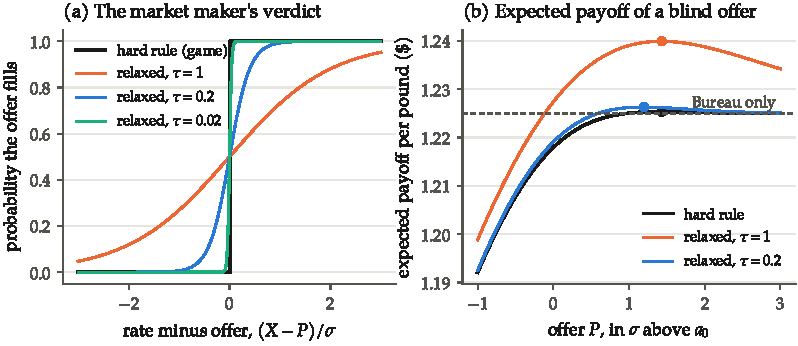
\includegraphics[width=\textwidth]{figures/fig_relax}
\caption{The acceptance jump and its relaxation. (a) The market maker's verdict as a function of how far the rate is above the offer: the game's hard rule and the logistic ramp \eqref{eq:sigmoid} at three temperatures. (b) The expected payoff of a pound seller's blind offer under the hard rule and the relaxed rule, with each maximum marked. At $\tau=1$ the relaxed game is far more generous than the real one; at $\tau=0.2$ it is close; the final temperature, $0.02$, is indistinguishable from the hard rule at this scale.}
\label{fig:relax}
\end{figure}

The relaxation changes the problem, and the anneal controls by how much. In the one blind offer game at the final temperature $\tau=0.02$, the optimum of the relaxed payoff lies \val{relax.shiftc}\,$\sigma$ from $P^*$ and its value differs by \val{relax.gainc} dollars per pound. At $\tau=0.2$ the optimum is \val{relax.shiftb}\,$\sigma$ away, and at $\tau=1$ the relaxed payoff overstates the value of an offer by \val{relax.gaina} dollars per pound, more than half of the fee. Early in training the agents play a smoother and more generous game than the real one; by the end they play nearly the real one. The remaining error at $\tau=0.02$, \val{relax.gainc} dollars per pound in this game, is larger than the whole one-offer edge at the rules' fees (\cref{sec:breakdown}), so the relaxation alone is enough to blur that edge.

\subsection{Policies}\label{sec:policies}
\paragraph{Traders}
Each trader's network sees the fraction of rounds left, the phase (offer or Bureau), its holdings of its starting currency as a share of $L$, its holdings of target currency as a share of $T$, the last revealed rate, and the last four rate moves. It is not told $a_0$ or $\sigma$. By \cref{sec:rate} the last revealed rate is a sufficient statistic for the rate, so the history adds nothing to a forecast of it; it may still say something about the other agents' positions. The network is a fully connected residual network: a 64-unit input layer, two residual blocks and a linear skip from the inputs, with GELU activations. In the offer phase it has two outputs: the price, $P=2\,a\,\mathrm{sig}(u_1)$ relative to the last revealed rate $a$, and a signed share $s=2\,\mathrm{sig}(u_2)-1$. For $s>0$ the trader offers the share $s$ of its starting currency; for $s<0$ it offers the share $|s|$ of its target currency back, so it may trade in either direction (\cref{sec:assumptions}). In the Bureau phase the same network gives the share of its remaining starting currency to convert.

\paragraph{Market maker}
The market maker's network has the same body. For each offer it sees the round's true rate, the fraction of rounds left, its own pound and dollar balances as shares of the game's capital (live or as at the start of the round, depending on the design below), the size and direction of the offer and, in the default design, the number of offers still to come in the round. It never sees who made the offer, and in the bid-wise and round-wise designs below it never sees the offer's price. It outputs an acceptance level $\ell=2X\,\mathrm{sig}(u_1)$ and accepts when $\delta\,(\ell-P)>0$, so learning the fee-aware rule of \cref{sec:rule} means learning $\ell=(1-g)X$ for pound sellers. In the Bureau phase it outputs the share of its short balance to repay at the Bureau, by selling the currency it is long in; repaying all of it flattens the position, and in round 5 it must repay what is left. Its level starts at $0.9X$ for pound sellers and $1.1X$ for dollar sellers, so that it begins by rejecting everything and must learn to trade.

\paragraph{Three market-maker designs}
Netting needs the market maker to use one trader's flow against another's within a round. How much of the round it can see when it decides could therefore matter. The rules have the offers presented one by one, which is the first design below; the other two change only how much of the round the market maker sees when it decides. The three share the network body, the training and the game; their inputs differ, so a difference between them reflects both the information and how hard each design is to learn.
\begin{itemize}
\item \emph{Bid-wise} (the default, and the game as played in the room). Slips arrive one at a time and each is answered before the next is seen. The acceptance level is set afresh for every offer from the book as it stands after the fills so far, and the market maker knows how many offers are still to come. It cannot hold an offer back to pair it with a later one: it is a dealer answering requests one by one.
\item \emph{Turn-wise.} The market maker reads every offer of the round, prices and sizes included, before giving any verdict, and decides against the book as it stood when the round opened. Its verdicts cannot depend on the arrival order, and it can accept two offers because they cross. It is not the real game. It sees every offer of the round, which the bid-wise market maker does not, but not the book as it changes within the round, which the bid-wise market maker does, so neither design contains the other.
\item \emph{Round-wise.} The level for each offer is set from the book as it stood when the round opened, from that offer's own size and direction only. The market maker knows nothing of the other offers in the round and does not update its book within the round. It is the simplest design and the reference for the other two.
\end{itemize}
If the bid-wise and turn-wise market makers net the same as the round-wise one, within-round information does not matter; \cref{sec:four} reports the comparison.

\subsection{Co-training}\label{sec:cotrain}
The agents are trained by alternating gradient play: each side takes a block of gradient steps against the other's latest policy. A block is an improvement, not a best response, and each side responds to the other's latest policy rather than, as in fictitious play, to the average of its past policies \citep{brown1951}. Such dynamics need not converge and can cycle \citep{balduzzi2018}; \cref{sec:cotrain-results,sec:four} show what the learning curves do. The market maker trains first, for \val{hp.inner} gradient steps against frozen traders; then the traders train for \val{hp.inner} steps against the frozen market maker; this is one outer step, and there are \val{hp.outer} of them (\cref{fig:loop}; settings in \cref{tab:params}). Every step draws \val{hp.batch} fresh games. The four traders update simultaneously, each on the gradient of its own score with the others' networks held fixed. A frozen agent still passes gradients through the game: a trader's gradient includes the market maker's response to its offer.

A trader maximises its expected P/L $(W-L)/L$ from \eqref{eq:terminal}; the market maker maximises its expected surplus in pounds at $a_5$ after the forced clear, as a share of the game's capital. We use AdamW \citep{loshchilov2019} with learning rate \val{hp.lrtrader} for the traders, halved when a trader's training loss stops improving, and a constant \val{hp.lrmm} for the market maker, with gradients clipped to norm one. \Cref{app:robustness} reports runs with the traders' rate cut to the market maker's. Every agent starts from a freshly initialised network; nothing is pre-trained. After each block the agents are scored on 20{,}000 fixed games of the hard game. Training stops early if the last four outer steps show no significant change; otherwise it runs all \val{hp.outer}, and the final networks are evaluated.

\begin{figure}[htb]
\centering
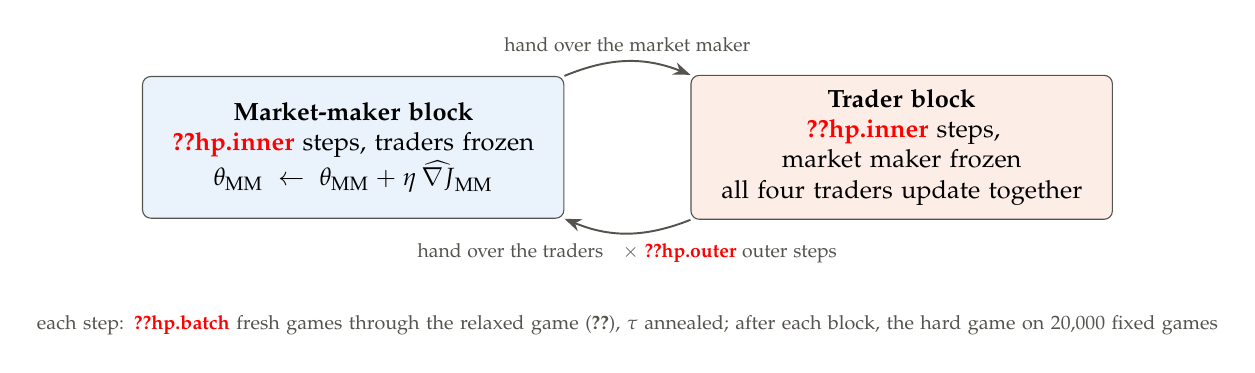
\begin{tikzpicture}[font=\small, >=Stealth, node distance=8mm and 16mm,
  blk/.style={draw=cink, rounded corners=3pt, align=center, inner sep=5pt, text width=50mm, minimum height=18mm,
               execute at begin node={\hyphenpenalty 10000 }},
  note/.style={font=\scriptsize, text=cink, align=center}]
  \node[blk, fill=cblue!10] (mm) {\textbf{Market-maker block}\\ \val{hp.inner} steps, traders frozen\\ $\theta_{\text{MM}} \leftarrow \theta_{\text{MM}}+\eta\,\widehat{\nabla J}_{\text{MM}}$};
  \node[blk, fill=corange!12, right=of mm] (tr) {\textbf{Trader block}\\ \val{hp.inner} steps, market maker frozen\\ all four traders update together};
  \draw[->, cink, line width=0.7pt] (mm.north east) to[bend left=22] node[above, note] {hand over the market maker} (tr.north west);
  \draw[->, cink, line width=0.7pt] (tr.south west) to[bend left=22] node[below, note] {hand over the traders\quad $\times$ \val{hp.outer} outer steps} (mm.south east);
  \node[note, below=11mm of $(mm.south)!0.5!(tr.south)$, text width=150mm, execute at begin node={\hyphenpenalty 10000 }] (n) {each step: \val{hp.batch} fresh games through the relaxed game \eqref{eq:sigmoid}, $\tau$ annealed; after each block, the hard game on 20{,}000 fixed games};
\end{tikzpicture}
\caption{Co-training by alternating gradient play. Each block improves one side against a fixed copy of the other; gradients flow through the frozen side's responses. $\theta_{\text{MM}}$ are the market maker's network weights, $\eta$ the learning rate and $\widehat{\nabla J}_{\text{MM}}$ the gradient of its expected score estimated on one batch of games (\cref{sec:direct}).}
\label{fig:loop}
\end{figure}

\subsection{Population training}\label{sec:population-method}
To test whether a market maker that has seen more counterparties nets more flow (\cref{h:population}), we also co-train market makers with random tables of $N=4$, $12$ or $24$ traders. Each random trader's side is a fair coin (the table is redrawn until both sides appear), its start is 50k, 100k, 200k or 500k units of its currency, its target is the fair value times a uniform draw from $[0.9,1.1]$, and each of its two penalties is drawn from $\{0,2,3,5,10,20\}\%$. The table is drawn once per run, so the market maker trains against one fixed table of $N$ traders, not a distribution of tables; testing it on T1--T4 is then a test on traders it has not seen. The table sizes were limited by hardware: every training step plays \val{hp.batch} games through all $N$ traders, so memory and run time grow with $N$, and tables much larger than 24 were not feasible on the machine available. The market maker trained against the table is then frozen, and T1--T4 are trained against it from fresh networks, exactly as in co-training but with the market maker fixed. As a control, the market maker co-trained with T1--T4 is put through the same procedure.

\subsection{Evaluation}\label{sec:eval}
All agents are evaluated on the hard game with common random numbers: the same 200{,}000 rate paths and arrival orders for every market maker and every comparison, so that differences are paired \citep{glasserman2004}. A trader's \emph{edge} is its P/L minus the P/L of converting everything at the Bureau in round 1 on the same path; edges are in bp of the trader's capital, and the market maker's P/L in bp of the game's capital. Flows are measured on 20{,}000 recorded games: the share of the game's money traded with the market maker, netted by it (its traded volume that never goes to the Bureau, counting both legs of a matched pair, so netted $=$ traded $-$ sent to the Bureau), sent by it to the Bureau, converted by the traders at the Bureau, and left unconverted. Uncertainties are two standard errors of the paired mean over evaluation paths, for the trained networks; they do not include the variation between training runs.

\begin{remark}[Model-free reinforcement learning]\label{rem:ppo}
A natural alternative is to treat the game as a Markov decision process and learn from rewards alone. In an untuned attempt with proximal policy optimisation \citep{schulman2017} on the single-trader game, the policy learned to use the Bureau both at the rules' trader fee of \val{p.f}, where the optimum over one round is only \val{ppo.R1.prize} bp better than the Bureau, and at a \val{ppo.R4.fee} fee, where the optimum over four rounds is \val{ppo.R4.prize} bp better. We did not pursue it. At the rules' fee the difficulty is statistical: the optimal blind offer beats the Bureau by \val{v0.edge} dollars per pound, \val{v0.edgeratio} standard deviations of a single game's payoff, so about \val{v0.ndetect} games are needed to see the difference at two standard errors. A pathwise gradient of the relaxed game sees the difference directly; a score-function gradient \citep{williams1992} must find it in the noise of the whole payoff. The failure at the higher fee is not explained by this argument and may be a matter of tuning.
\end{remark}

%%% ---- sections/s7_results ----
% =============================================================================
\section{Results}\label{sec:results}
% =============================================================================
We first check the method against the dynamic-programming solutions of \cref{sec:exact,sec:fee} (\cref{sec:validation,sec:carry-learned}), then let one trader and one market maker learn together (\cref{sec:cotrain-results}), and finally study the four-trader market (\cref{sec:four,sec:ladder,sec:population,sec:mechanism}).

\subsection{Validation against the dynamic programme}\label{sec:validation}
\paragraph{Traders}
We trained a single-trader network for T1 and for T2 against the flatten-rule market maker of \cref{sec:rule} at each of the four fee pairs, and replayed both the network and the dynamic-programming policy on the same 200{,}000 games (the last two columns of \cref{tab:feedp}; edges as in \cref{sec:eval}).

For the pound seller the network comes within \val{dp.A.maxreg} bp of capital of the dynamic programme at every fee pair (\cref{tab:feedp}). The $(2\%,1\%)$ rows test nothing: there is almost nothing to win, and a policy that only used the Bureau would pass them.

The dollar seller is validated less well: where its channel is open the network falls \val{dp.B.regmin} to \val{dp.B.regmax} bp short of the programme, and at $(3\%,1\%)$ its edge cannot be told from the Bureau floor while the programme's can (\cref{tab:feedp}). The programme's own edge at $(2\%,0)$ is only about three standard errors from zero.

The one-sided martingale (\cref{prop:siegel}) suggests why. Waiting a round costs the pound seller \val{floor.perround} bp (\cref{sec:martingale}), so converting in round 1 stands far above the alternatives. It costs the dollar seller only \val{floorB.perround} bp (\cref{sec:carry}), so many of its policies are worth within a few basis points of each other, and those that carry make its P/L far noisier (compare the error bars in \cref{tab:feedp}). A gradient estimated from \val{st.batch} games cannot separate policies that close. We have not tested this explanation directly.

\paragraph{Market maker}
We trained a market-maker network against a fixed trained trader, with and without its own fee, and compared it with four threshold rules: accept when $P<X$ (\emph{naive}) or $P<(1-g)X$ (\emph{fee-aware}) for a pound seller, mirrored for a dollar seller, each either flattening every round or carrying to round 5. The network earns at least what the best rule earns, less at most \val{mmn.maxshort} bp, and its verdicts agree with the threshold rule's on every recorded offer (\cref{tab:mmnet}); where it beats the best rule, against the dollar seller at $g=0$, the gain therefore comes from the timing of its Bureau conversions. At $g=1\%$ the market maker earns almost nothing, so \cref{h:threshold} is tested more sharply by co-training (\cref{sec:cotrain-results}).

\begin{table}[htb]
\centering\footnotesize\setlength{\tabcolsep}{4.5pt}
\begin{threeparttable}
\caption{The market-maker network against the best of four threshold rules, trained and evaluated against a fixed trained trader. The trader's fee is fixed at $f=\val{p.f}$; $g$ is the market maker's. P/L in basis points of capital; the difference is paired, $\pm$ two standard errors. The last column counts recorded offers on which the network's verdict differs from the threshold rule's.}
\label{tab:mmnet}
\begin{tabular}{lrlrrr}
\toprule
case & network & best rule & rule & network $-$ rule & disagreements\\
\midrule
\tablebody{tables/tab_mmnet.tex}
\bottomrule
\end{tabular}
\end{threeparttable}
\end{table}

\subsection{Flatten or carry: the one-sided martingale learned}\label{sec:carry-learned}
The market maker is scored in pounds, so the premium of \cref{prop:siegel} is part of its score, and its learned Bureau policy follows the asymmetry of \cref{rem:carrymm}. Without a fee of its own, facing a pound seller, whose fills leave it short of dollars, the network flattens \val{mmn.A0.repay1} of its open position in round 1; facing a dollar seller, whose fills leave it long dollars, it flattens \val{mmn.B0.repay1} and carries the rest. The reference rules rank the same way: against the pound seller flattening earns \val{mmn.A0.nvflatten} bp and carrying \val{mmn.A0.nvcarry}; against the dollar seller carrying earns \val{mmn.B0.nvcarry} and flattening \val{mmn.B0.nvflatten}. The force that makes T1 convert early and T2 carry (\cref{sec:carry}) also decides how the market maker runs its book.

\subsection{One trader and one market maker learning together}\label{sec:cotrain-results}
Before adding more traders, we check that one trader and one market maker learning together from fresh networks reach the outcome the dynamic programme predicts (\cref{h:cotrain,tab:cotrain}); if they did not, a four-trader result could not be told apart from a failure of the learning.

At the rules' fees the market closes, as \cref{h:cotrain} predicts, though this cell is not a sharp test: the learner cannot resolve an edge as small as the dynamic programme's there (\cref{sec:relax}). At $(2\%,0)$ and $(3\%,1\%)$ the market stays open, and the pound seller's edges are close to the programme's against the flatten rule (\cref{tab:cotrain,tab:feedp}). The market maker learns the threshold rule, supporting \cref{h:threshold}: its fitted round-1 level for a pound seller is $\val{co.Ag0.thr1}\,X$ at $g=0$ and $\val{co.Ag1f3.thr1}\,X$ at $g=\val{p.g}$, the naive and fee-aware rules.

The dollar seller's market maker carries. At $(3\%,1\%)$ its level, $\val{co.Bg1f3.thr1}\,X$, lies between the price at which a flattening market maker breaks even, $X/(1-g)=\val{carry.flatB}\,X$, and the lower price at which a carrying one does, $\val{carrymm.break}\,X$ (\cref{rem:carrymm}): it accepts offers that flattening would reject. The trader's edge also beats the dynamic programme's against a flattening market maker (\cref{tab:cotrain,tab:feedp}).

Over the last ten blocks of training the pound seller's edge moves by less than the noise of one measurement; the dollar seller's swings by tens of basis points, as \cref{sec:validation} suggests, so its numbers in \cref{tab:cotrain} are snapshots of a moving policy (\cref{tab:learnrange}, \cref{app:learning}). At $(2\%,0)$ the snapshot falls below the Bureau floor, but over the last ten blocks the edge ranges from just below the floor to far above the programme's, and the run stopped near the bottom of that range.

\begin{table}[htb]
\centering\small
\begin{threeparttable}
\caption{One trader and one market maker co-trained from fresh networks, evaluated on the hard game on the 200{,}000 evaluation games (\cref{tab:learnrange} uses the 20{,}000 validation games, so its final values differ slightly). Market-maker P/L in basis points of capital; trader edge over the Bureau in bp of capital, $\pm$ two standard errors; the share of offered volume that fills; the market maker's fitted acceptance level in round 1 as a multiple of $X$; and the agreement of its verdicts with the benchmark threshold rule.}
\label{tab:cotrain}
\begin{tabular}{lrrrrr}
\toprule
trader, $(f,g)$ & MM P/L & trader edge & filled & level$/X$ & agreement\\
\midrule
\tablebody{tables/tab_cotrain.tex}
\bottomrule
\end{tabular}
\begin{tablenotes}\footnotesize
\item Where almost nothing fills, the level is not tested by any offer and is not identified.
\end{tablenotes}
\end{threeparttable}
\end{table}

\subsection{Four traders}\label{sec:four}
With T1--T4 co-trained with a market maker at the rules' fees, a spread of $f-g=1\%$, there is no trade: \val{lad.s10.anyfill} of games see a fill, and the traders park their offers far from the rate, the median pound seller's \val{mech.s10.qpound} and the median dollar seller's \val{mech.s10.qdollar} from the last revealed rate. The one-trader breakdown of \cref{sec:fee} survives counterparties on both sides; as in \cref{sec:cotrain-results}, this is consistent with the dynamic programme rather than a sharp test of it.

At a 2\% spread, $(f,g)=(3\%,1\%)$, the fee pair of \cref{sec:fullfee}, there is trade (\cref{fig:learning} in \cref{app:learning}). From block 10 on, the market maker's P/L stays within \val{learn4.mmgap} bp of the best of six fixed rules played against the same traders, including a book rule that tries every subset of the round's offers, so at each block it is about as good a response to the current traders as any of them. The agents oscillate rather than reach a fixed point: over the last ten blocks the pound sellers' edges move within a few basis points, the dollar sellers' by tens and the market maker's P/L by over 20 bp, several times the noise of a measurement, but over the recorded blocks every curve stays within a band (\cref{tab:learnrange4}). As with one trader, the dollar sellers move most. Every number reported for this market is a snapshot of the final networks within that oscillation.

The bid-wise and turn-wise market makers trade and net similar shares of the money at a 2\% spread, and the difference in netting lies inside the bid-wise run's range across seeds, \val{rob.seed242.netted} to \val{lad.s20.netted} (\cref{tab:arms}): in these single runs, seeing the whole round did not lead to more netting, though one run per design cannot isolate the value of that information. The round-wise market maker essentially never trades, though it can represent the fee-aware rule, which needs no information from within the round, so its failure is one of learning in that run, not a limit of the design. No trader uses the option to trade back: the share of filled volume traded in the reverse direction is \val{mech.s20.revfilled}.

\begin{table}[htb]
\centering\small
\begin{threeparttable}
\caption{The three market-maker designs of \cref{sec:policies}, each co-trained with T1--T4, one run per design and spread. Shares of the game's money on 20{,}000 recorded games; market-maker P/L in bp of the game's capital on 200{,}000.}
\label{tab:arms}
\begin{tabular}{llrrr}
\toprule
spread & design & MM trades & netted & MM P/L\\
\midrule
\tablebody{tables/tab_arms.tex}
\bottomrule
\end{tabular}
\end{threeparttable}
\end{table}

\subsection{Widening the fee spread}\label{sec:ladder}
To find what reopens the market, we co-train T1--T4 with a market maker at each spread $f-g$ from 1\% to 6\%, raising the traders' Bureau fee $f$ with the market maker's fixed at \val{p.g} (\cref{tab:ladder,tab:gains,fig:ladder}).

\begin{table}[H]
\centering\footnotesize\setlength{\tabcolsep}{4.5pt}
\begin{threeparttable}
\caption{The four-trader market as the fee spread widens: trader fee $f$ from 2\% to 7\%, market-maker fee $g=\val{p.g}$, one co-training run per spread. Flows are shares of the game's money on 20{,}000 recorded games; market-maker P/L in basis points of capital on 200{,}000.}
\label{tab:ladder}
\begin{tabular}{lrrrrrrr}
\toprule
spread & MM trades & netted & MM to Bureau & traders to Bureau & left & all Bureau & MM P/L\\
\midrule
\tablebody{tables/tab_ladder.tex}
\bottomrule
\end{tabular}
\begin{tablenotes}\footnotesize
\item MM trades $=$ netted $+$ MM to Bureau, and all Bureau $=$ MM to Bureau $+$ traders to Bureau. Volumes are valued in pounds at the rate at which each trade happens: a filled dollar offer at its price, a Bureau conversion at that round's rate, money left over at $a_5$. Valued at $a_0$, MM trades, traders to Bureau and left would sum to exactly 100\%; at the trade rates they sum to between \val{lad.summin} and \val{lad.summax}. With no trade the sum is slightly above 100\%, because the dollar sellers' money converted at the round's rate picks up the premium of \cref{prop:siegel}.
\end{tablenotes}
\end{threeparttable}
\end{table}

\begin{table}[H]
\centering\small
\begin{threeparttable}
\caption{Each trader's gain over converting everything at the Bureau in round 1, in bp of its capital, $\pm$ two standard errors, as the fee spread widens; one co-training run per spread, on the 200{,}000 evaluation games. From the 4\% spread on, the gains include the value of not converting.}
\label{tab:gains}
\begin{tabular}{lrrrr}
\toprule
spread & T1 & T2 & T3 & T4\\
\midrule
\tablebody{tables/tab_gains.tex}
\bottomrule
\end{tabular}
\end{threeparttable}
\end{table}

\begin{figure}[H]
\centering
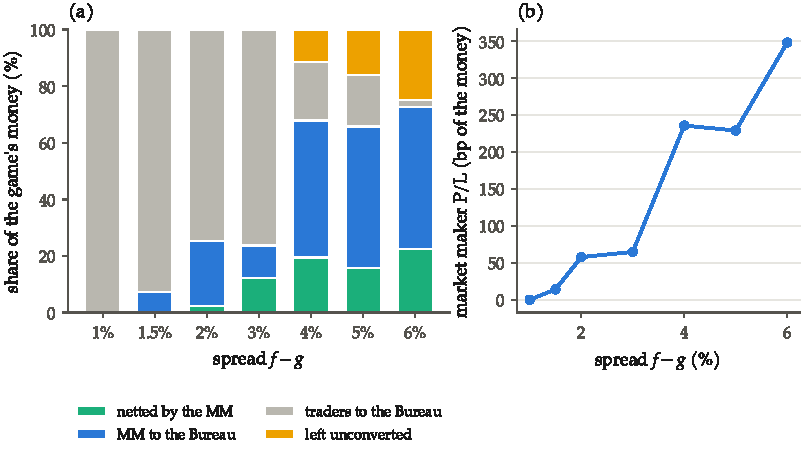
\includegraphics[width=\textwidth]{figures/fig_ladder}
\caption{(a) Where the game's money goes as the spread $f-g$ widens, normalised to 100\%. (b) The market maker's P/L. One co-training run per spread (\cref{tab:ladder}).}
\label{fig:ladder}
\end{figure}

The market opens between 1\% and 1.5\%: at 1.5\% \val{lad.s15.anyfill} of games see a fill. The one-trader analysis predicts this: the best single offer fills \val{fee.fill21} of the time at a 1\% spread and \val{fee.fill251} at 1.5\% (\cref{fig:rho}). Netting grows with the spread, though not monotonically, which supports \cref{h:spread}.

At a 2\% spread every agent gains: the market maker earns \val{lad.s20.mmpl} bp and every trader beats the Bureau. At 6\% the market maker earns \val{lad.s60.mmpl} bp, and T4 is the one trader that does worse than the Bureau.

From the 4\% spread, where $f=5\%$, money is left unconverted; at 6\% about as much is left as is netted. Converting one unit short of the target gains $\alpha+\beta-f(1+\beta)$ in the starting currency at an unchanged rate, which is negative once $f$ exceeds $(\alpha+\beta)/(1+\beta)$: \val{left.fT1} for T1 and \val{left.fT2} for T2. Above these fees the traders stop converting, so their gains in \cref{tab:gains} include the value of not converting.

\FloatBarrier
\subsection{More counterparties}\label{sec:population}
If the market maker nets little because it has seen only four counterparties, training it against more should help (\cref{h:population}). We trained one market maker on a random table of 4, 12 and 24 traders each, froze it, and trained T1--T4 against it from fresh networks. As a control, the market maker co-trained with T1--T4 went through the same test (\cref{sec:population-method}). In these runs more counterparties did not help (\cref{tab:population,fig:population}), but each size uses one random table, so the size of the table and its composition change together. At the rules' 1\% spread none of these market makers trades with T1--T4. At a 2\% spread they net \val{pop.test4b.netted}, \val{pop.test12b.netted} and \val{pop.test24b.netted} of the money, against \val{pop.frozen.netted} for the control, with no trend in $N$. They also trade less than the control: \val{pop.test4b.trades}, \val{pop.test12b.trades} and \val{pop.test24b.trades} of the money, against \val{pop.frozen.trades}. Tables larger than 24 traders were beyond the hardware available; \cref{sec:highN} discusses them.

\begin{table}[htb]
\centering\footnotesize\setlength{\tabcolsep}{4.5pt}
\begin{threeparttable}
\caption{Market makers trained on random tables of traders, then frozen and tested against freshly trained T1--T4, at a 2\% spread. The control is the market maker co-trained with T1--T4, frozen and put through the same test. Shares of the game's money, valued as in \cref{tab:ladder}; all Bureau is below 100\% by what is netted and what is left, up to that valuation. P/L in basis points.}
\label{tab:population}
\begin{tabular}{lrrrrr}
\toprule
market maker & MM trades & netted & MM to Bureau & all Bureau & MM P/L\\
\midrule
\tablebody{tables/tab_population.tex}
\bottomrule
\end{tabular}
\end{threeparttable}
\end{table}

\begin{figure}[htb]
\centering
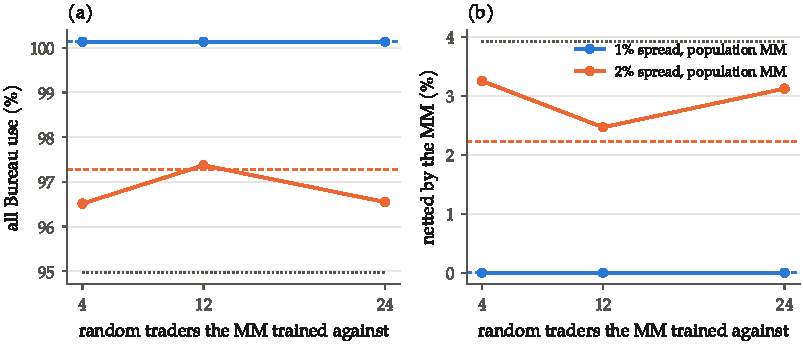
\includegraphics[width=\textwidth]{figures/fig_population}
\caption{Market makers co-trained with $N$ random traders, then frozen and tested against T1--T4: (a) all Bureau use; (b) netting. Blue: the rules' 1\% spread, where there is no trade and all the money goes to the Bureau (slightly above 100\%, for the valuation reason in the note to \cref{tab:ladder}). Orange: the 2\% spread of \cref{tab:population}. Dashed lines: the market maker co-trained with T1--T4. Dotted: the same market maker frozen and put through the test (the control), at 2\%.}
\label{fig:population}
\end{figure}

\FloatBarrier
\subsection{Mechanism: fills in opposite tails}\label{sec:mechanism}
Why does a market maker with flow on both sides net so little? To net within a round it needs a pound seller and a dollar seller to fill in the same round. Under the fee-aware rule of \cref{sec:rule}, a pound seller's offer at $P_A$ fills only when the rate is high, $X>P_A/(1-g)$, and a dollar seller's offer at $P_B$ only when it is low, $X<(1-g)P_B$. Both fill only if
\[
  \frac{P_A}{1-g} < X < (1-g)\,P_B,
\]
which needs $P_A<(1-g)^2P_B$: the pound seller must ask for fewer dollars per pound than the dollar seller offers, by about twice the fee. This is stricter than the quotes crossing, $P_A<P_B$ (\cref{rem:matched}): quotes that cross by less than this can be matched at a profit but cannot both pass the fee-aware rule. Quotes that do not cross at all, $P_A\ge P_B$, are worse: filling both loses $P_A-P_B$ dollars on every pound matched, whatever the rate, so a market maker that refuses a sure loss never fills both for the matched amount (\cref{fig:cross}).

\begin{figure}[htb]
\centering
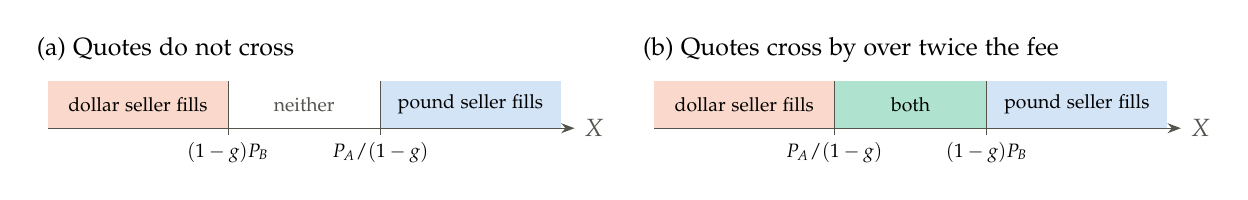
\begin{tikzpicture}[font=\small, >=Stealth, x=0.88cm, y=1cm]
  % (a) quotes do not cross
  \node[anchor=west, font=\small] at (0,1.0) {(a) Quotes do not cross};
  \fill[corange!25] (0.3,0) rectangle (2.9,0.6);
  \fill[cblue!20]   (5.1,0) rectangle (7.7,0.6);
  \draw[->, cink] (0.3,0) -- (7.9,0) node[right] {$X$};
  \draw[cink] (2.9,-0.08) -- (2.9,0.6); \node[below, font=\scriptsize] at (2.9,-0.05) {$(1-g)P_B$};
  \draw[cink] (5.1,-0.08) -- (5.1,0.6); \node[below, font=\scriptsize] at (5.1,-0.05) {$P_A/(1-g)$};
  \node[font=\scriptsize, align=center] at (1.6,0.3) {dollar seller fills};
  \node[font=\scriptsize, align=center] at (6.4,0.3) {pound seller fills};
  \node[font=\scriptsize, text=cink] at (4.0,0.3) {neither};
  % (b) quotes cross
  \begin{scope}[xshift=7.7cm]
  \node[anchor=west, font=\small] at (0,1.0) {(b) Quotes cross by over twice the fee};
  \fill[corange!25] (0.3,0) rectangle (5.1,0.6);
  \fill[cblue!20]   (2.9,0) rectangle (7.7,0.6);
  \fill[caqua!35]   (2.9,0) rectangle (5.1,0.6);
  \draw[->, cink] (0.3,0) -- (7.9,0) node[right] {$X$};
  \draw[cink] (2.9,-0.08) -- (2.9,0.6); \node[below, font=\scriptsize] at (2.9,-0.05) {$P_A/(1-g)$};
  \draw[cink] (5.1,-0.08) -- (5.1,0.6); \node[below, font=\scriptsize] at (5.1,-0.05) {$(1-g)P_B$};
  \node[font=\scriptsize] at (1.6,0.3) {dollar seller fills};
  \node[font=\scriptsize] at (6.4,0.3) {pound seller fills};
  \node[font=\scriptsize] at (4.0,0.3) {both};
  \end{scope}
\end{tikzpicture}
\caption{When both sides fill, under the fee-aware rule: the rates $X$ at which the market maker accepts a dollar seller's offer at $P_B$ (low rates) and a pound seller's offer at $P_A$ (high rates). (a) A pound seller quoting above the last revealed rate and a dollar seller quoting below it: no rate fills both. (b) Quotes that cross by more than twice the fee: a band of rates fills both, and the market maker nets the matched part with no Bureau fee and a sure gain (\cref{rem:matched}).}
\label{fig:cross}
\end{figure}

The traders, who cannot see the rate, quote on opposite sides of it, so their quotes do not cross (\cref{tab:fills}). At a 2\% spread the median pound seller's quote is \val{mech.s20.qpound} and the median dollar seller's \val{mech.s20.qdollar}, relative to the last revealed rate. A pound seller therefore fills only after the rate has risen (\val{mech.s20.uppound} of its fills) and a dollar seller only after it has fallen (\val{mech.s20.downdollar}). Pound sellers fill in \val{mech.s20.ppound} of rounds, but never in the same round as a dollar seller (both fill in \val{mech.s20.both} of rounds; \cref{tab:fills,fig:mechanism}): the rate that makes one side fill stops the other.

\begin{figure}[htb]
\centering
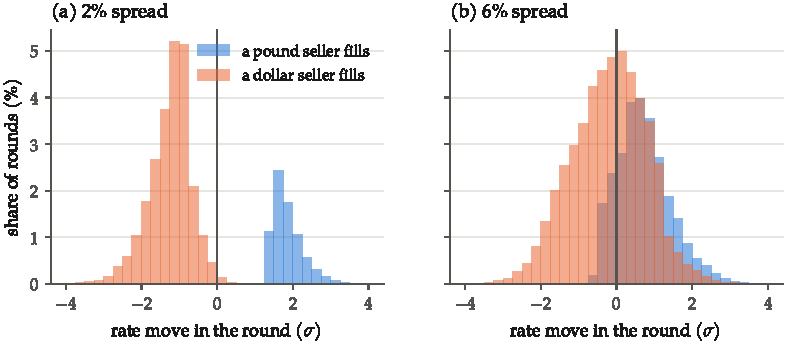
\includegraphics[width=\textwidth]{figures/fig_mechanism}
\caption{How far the rate had moved, in units of $\sigma$, in the rounds in which a pound seller's offer filled and in those in which a dollar seller's did, as a share of all rounds, at (a) a 2\% and (b) a 6\% spread. At 2\% pound sellers fill only after the rate has risen and dollar sellers only after it has fallen, so no round has both, as in \cref{fig:cross}a. At 6\% the two overlap: when the rate moves little, both sides fill, as in \cref{fig:cross}b. One co-training run per spread.}
\label{fig:mechanism}
\end{figure}

\begin{table}[htb]
\centering\footnotesize\setlength{\tabcolsep}{4.5pt}
\begin{threeparttable}
\caption{Where the four traders quote and when they fill, one co-training run per spread, on the 20{,}000 recorded games. Median quotes of the pound sellers and the dollar sellers relative to the last revealed rate, over all offers and over filled offers only; and the share of rounds in which a pound seller fills, a dollar seller fills, and both fill in the same round.}
\label{tab:fills}
\begin{tabular}{lrrrrrrr}
\toprule
 & \multicolumn{2}{c}{median quote} & \multicolumn{2}{c}{median filled quote} & \multicolumn{3}{c}{rounds with a fill}\\
\cmidrule(lr){2-3}\cmidrule(lr){4-5}\cmidrule(lr){6-8}
spread & pound & dollar & pound & dollar & pound & dollar & both\\
\midrule
\tablebody{tables/tab_fills.tex}
\bottomrule
\end{tabular}
\end{threeparttable}
\end{table}

What little the market maker nets, it nets across rounds: it carries what it buys and flattens only at the end (\val{mech.s20.final} of its Bureau volume is the final clear), so a purchase in one round can offset a sale in a later one. Its Bureau use is then close to the imbalance of its fills: it sends \val{lad.s20.bshare} of its trades to the Bureau, and the imbalance between what it bought and what it sold is \val{mech.s20.imb}. The cards limit this too: \val{cards.dollarshare} of the money starts in dollars, so even if every offer filled, at most \val{cards.nettable} of it could be netted.

As the spread widens the two sides start to fill together: both fill in the same round in \val{mech.s30.both}, \val{mech.s40.both} and \val{mech.s50.both} of rounds at 3, 4 and 5\%, and the median filled quotes cross from 5\% (\cref{tab:fills}). At 6\% pound sellers fill in \val{mech.s60.ppound} of rounds, and in \val{mech.s60.both} of rounds a dollar seller fills in the same round, so almost every pound fill comes with a dollar fill (\cref{tab:fills,fig:mechanism}). The market maker then nets \val{lad.s60.netted} of the money, as much as its fills could match at most (\val{lad.s60.matchable}, twice the smaller of what it bought and what it sold; the small excess comes from valuing trades at different rates).

\FloatBarrier
\subsection{The hypotheses}\label{sec:verdicts}
\Cref{tab:verdicts} sets each hypothesis of \cref{sec:hypotheses} against the result that tests it.

\begin{table}[htb]
\centering\small
\begin{threeparttable}
\caption{The hypotheses of \cref{sec:hypotheses} and what the experiments found.}
\label{tab:verdicts}
\begin{tabularx}{\textwidth}{@{}l>{\raggedright\arraybackslash}p{0.27\textwidth}l>{\raggedright\arraybackslash}X@{}}
\toprule
 & hypothesis & verdict & evidence\\
\midrule
\ref{h:threshold} & a learned market maker recovers the threshold rule & supported for pound sellers & against a pound seller its level is $\val{co.Ag0.thr1}\,X$ at $g=0$ and $\val{co.Ag1f3.thr1}\,X$ at $g=\val{p.g}$; against a dollar seller it carries instead, which earns more (\cref{sec:validation,sec:carry-learned,sec:cotrain-results})\\
\ref{h:cotrain} & one-trader co-training breaks down at $(2\%,1\%)$ only & supported & no trade at $(2\%,1\%)$; at $(2\%,0)$ and $(3\%,1\%)$ the market stays open (\cref{tab:cotrain}); the closed cell is not a sharp test\\
\ref{h:net} & with both sides, the market maker nets & partly & not at the rules' fees, where nothing trades; little at a 2\% spread; clearly from 3\% (\cref{tab:ladder})\\
\ref{h:population} & more counterparties, more netting & not supported & no trend for $N=4$, 12, 24 (\cref{sec:population})\\
\ref{h:spread} & a wider spread, more netting & supported & netting rises from nothing at 1\% to \val{lad.s60.netted} at 6\%, not monotonically; one run per spread (\cref{tab:ladder})\\
\bottomrule
\end{tabularx}
\end{threeparttable}
\end{table}

%%% ---- sections/s8_discussion ----
% =============================================================================
\section{Discussion}\label{sec:discussion}
% =============================================================================

\subsection{What makes the market maker net}\label{sec:answer}
The research question asked what incentivises the market maker to clear its book by matching traders rather than through the Bureau. For the model of this paper and, in the multi-agent part, for this learning procedure, the answer comes in three steps. First, there must be flow. A trader offers to an informed market maker only if the fee it can save is large beside a step of the rate. At the rules' fees the governing ratio is $\rho=\val{fee.rho21}$, the best blind offer fills \val{fee.fill21} of the time, and with one offer per round the policy the dynamic programme finds is worth less than a basis point of capital more than the Bureau (\cref{sec:fee}). With four learning traders the market is as empty: \val{lad.s10.anyfill} of games see a fill (\cref{sec:four}). A market maker with no flow has nothing to net. Second, flow on both sides is not enough. Blind quotes are filled in opposite tails of the rate, so a pound seller and a dollar seller almost never fill in the same round (\cref{sec:mechanism}). The market maker can net only by carrying one side's position until the other side's fill arrives, or when the traders' quotes cross, and both need a wide spread. Third, in our runs more counterparties did not substitute for a spread (\cref{sec:population}).
The incentive the rules intend, small margins on a large volume, therefore does not get started at the rules' fees in this model: the volume it needs is not there. What creates it is the gap between the traders' fee and the market maker's, measured against the volatility of the rate.

\subsection{Trade and no trade in the learning dynamics}\label{sec:equilibria}
Is the absence of trade at the rules' fees a property of the game, or did the learning simply fail to find trade? Every co-training run does find trade at first: the market maker trains first, against untrained traders whose offers sit near the rate, and accepts many of them, so in every run, at either spread, at least \val{curve.s10.peaklo} of offered volume fills within the first three blocks (for the base 2\% run, see \cref{fig:learning}). What happens next depends on the spread. At 1\% every run ends with no trade (\cref{tab:ladder,fig:population}). At 2\% every run ends trading (\cref{tab:ladder,tab:population,tab:robust}) except the one in which neither agent's acceptance rule was smoothed: its rule stays close to the hard rule, so once its fills stopped there was no gradient to restart them (\cref{sec:relax}).

No trade is a Nash equilibrium of the game: if the market maker rejects everything, no offer beats the Bureau, and if no acceptable offer arrives, rejecting costs the market maker nothing. It is a fragile one, since a market maker that rejects an offer it could flatten at a profit gives up a sure gain in that round. At 1\% no trade is also close to what the game predicts, since the dynamic programme finds almost nothing to trade (\cref{tab:feedp}). At 2\% it is not: a trader facing a fee-aware market maker gains by offering, so a run that closes there has stalled rather than found the game's outcome. Two experiments would separate the two more sharply: starting the 1\% market from agents already trading at 2\%, which should still close if the game forces it, and starting the 2\% market from a market maker that already follows the fee-aware rule, which should stay open.

\subsection{Far larger markets: a hypothesis}\label{sec:highN}
Our population runs stop at $N=24$ because of hardware (\cref{sec:population-method}). Far larger markets might net where ours do not. A market maker learns its acceptance level only from offers near that level, and a very large volume of trades could let it learn to accept on a thin margin, which is the incentive the rules intend; with many cards, quotes are also more dispersed, and more of them could cross (\cref{rem:matched}). The case against is the mechanism of \cref{sec:mechanism}: fills are driven by the common rate, so when the rate rises pound sellers fill and dollar sellers do not, however many there are, and this dependence does not average out with $N$. Large $N$ helps netting only if it makes quotes cross. Testing this needs more computing power or the mean-field limit of the market (\cref{sec:conclusion}).

\subsection{The numéraire}\label{sec:numeraire}
Scoring each trader in its own starting currency was meant to make the game symmetric, but \cref{prop:siegel} shows that it cannot be. The premium is small, \val{kappa.onebonus} per round held, yet it decides who converts early and who carries in the dynamic-programming solution (\cref{sec:carry}), how the learned market maker runs its book (\cref{sec:carry-learned}), and on which side the dynamic programme's grid bias appears (\cref{sec:bias}).

\subsection{Implications for the exercise}\label{sec:implications}
In this model, with one offer per round against a market maker that flattens, the policy we find at the rules' fees is worth less than a basis point of capital more than the Bureau, and a market maker that understands its own fee has almost nothing to gain from the traders. Two changes reopen the market. A spread between the traders' fee and the market maker's of 1.5\% or more let a market form in our runs (\cref{sec:ladder}); a calmer rate works the same way through $\rho$, and halving $\sigma$ at the rules' fees restores the one blind offer fill probability to \val{fee.fillhalfsd} (\cref{sec:breakdown}). Letting traders make several offers per round, as the room in fact allows, also gives them something (\cref{app:sequential}).

\subsection{Limitations}\label{sec:limitations}
\begin{itemize}
\item \emph{Model.} The rate is an additive Gaussian walk with known $\sigma$; every agent is risk neutral; each trader makes one offer per round, although the rules allow more, and the several-offer results of \cref{app:sequential} assume a market maker that does not act strategically on probes; and the benchmark market maker flattens every fill, which against dollar sellers earns less than carrying (\cref{rem:carrymm}).
\item \emph{Replication.} The fee-spread ladder, the market-maker designs and the population sizes use one co-training run each. Across three seeds of the 2\% run, the market maker's Bureau use ranges from \val{rob.seed242.mmbdc} to \val{lad.s20.mmbdc} of the money and netting from \val{rob.seed242.netted} to \val{lad.s20.netted} (\cref{app:robustness}), so differences smaller than that should not be read.
\item \emph{Convergence.} Alternating gradient play need not reach a fixed point in a game \citep{balduzzi2018}, and ours does not: the pound sellers settle, but the dollar sellers and the market maker oscillate within a band over the recorded blocks (\cref{app:learning}), and the base 2\% run never met its stopping rule. We have not measured the exploitability of the final profile, how much each agent could gain by training alone against the others \citep{lanctot2017}.
\item \emph{Validation.} Single-trader networks were checked against the dynamic programme only for T1 and T2, and the dollar seller's network captures only part of the programme's edge (\cref{sec:validation}), so the dollar sellers' flow, and with it netting, may be understated.
\item \emph{Numerics.} Dynamic-programming values are values of computed policies, so they are lower bounds; outside the threshold grid we bound what is missed (\cref{app:numerics}), but we have no upper bound on what finer grids could add.
\item \emph{Design.} Raising the traders' fee also changes the cards' incentives to convert; a sweep in $\sigma$ would isolate $\rho$. The market maker's learning rate is ten times smaller than the traders', and we varied this only at 2\%, where cutting the traders' rate to the market maker's cuts trade from \val{lad.s20.trades} to \val{rob.lr.trades} of the money (\cref{tab:robust}). Population sizes were limited by hardware to $N\le24$, and each population run draws its table once.
\item \emph{Cards.} \val{cards.dollarshare} of the money is on the dollar side, which caps netting at \val{cards.nettable}; other tables may behave differently.
\end{itemize}

%%% ---- sections/s9_conclusion ----
% =============================================================================
\section{Conclusion}\label{sec:conclusion}
% =============================================================================
This paper studied a classroom FX market in which an informed market maker trades with uninformed traders who can always fall back on a Bureau. One blind offer has a closed form, the full single-trader game was solved by dynamic programming, and the market maker's own fee was shown to be a change of units in the trader's problem, governed by $\rho=\fp a_0/\sigma$. With one offer per round and a market maker that flattens each fill, the policy the dynamic programme finds gains less than a basis point of capital over the Bureau at the rules' fees, a lower bound on what is achievable; with several offers per round it need not be (\cref{app:sequential}). Neural policies trained by differentiating through a relaxed version of the game reproduced the dynamic programme for the pound seller, less well for the dollar seller, and were then used in a market of four traders and a market maker that all learn. In single runs there, in which the dollar sellers and the market maker oscillate within a band, trade appeared at a fee spread of 1.5\% but not at 1\%, and the market maker netted mostly by carrying inventory across rounds, because blind quotes fill in opposite tails of the rate.

Several extensions follow. The multi-agent results need more seeds, the exploitability of the final profile, and the two experiments of \cref{sec:equilibria}; the single-trader results need an upper bound, or a convergence study in the grids, at the rules' fees. The single-trader benchmark could use a market maker that carries as well as flattens, and several offers per round with a market maker that may wait. The rate model could be replaced by a log-normal rate, for which $\E[1/X]$ exists, a continuous-time limit, or unknown volatility. As the number of traders grows, a mean-field approximation with one dominant market maker may be useful \citep{carmona2018}; formulating it is open. Finally, the learned policies could be compared with the decisions made by students in the exercise.


\renewcommand{\bibfont}{\small}
\setlength{\bibsep}{1.5pt plus 0.5pt}
\bibliographystyle{plainnat}
\bibliography{refs}

\appendix
%%% ---- sections/appendix ----
% =============================================================================
\section{Parameters}\label{app:parameters}
% =============================================================================
By L\'evy's inequality for symmetric random walks, the chance that any of the five rates is non-positive is at most twice the chance that the last one is (\cref{tab:negative}, \cref{rem:negative}).

\begin{table}[!htb]
\centering\small
\begin{minipage}[t]{0.58\textwidth}
\centering
\captionof{table}{Game parameters and training settings, read from the saved evaluation file of the base 2\% run.}
\label{tab:params}
\footnotesize\setlength{\tabcolsep}{3pt}
\begin{tabular}{@{}llr@{}}
\toprule
\multirow{6}{*}{game} & initial rate $a_0$ (\$ per \pounds) & \val{p.a0}\\
 & step deviation $\sigma$ & \val{p.sd}\\
 & trader fee $f$ (rules) & \val{p.f}\\
 & market-maker fee $g$ (rules) & \val{p.g}\\
 & trading rounds, settlement & 4, 1\\
 & capital of the cards (\pounds) & \val{cards.capital}\\
\midrule
\multirow{8}{*}{co-training} & outer steps & \val{hp.outer}\\
 & gradient steps per block & \val{hp.inner}\\
 & games per gradient step & \val{hp.batch}\\
 & learning rate, traders / MM & \val{hp.lrtrader} / \val{hp.lrmm}\\
 & temperature, traders & \val{hp.tautrader0} $\to$ \val{hp.tautrader1}\\
 & temperature, MM & \val{hp.taumm0} $\to$ \val{hp.taumm1}\\
 & share spent annealing & \val{hp.anneal}\\
 & training games per agent & \val{hp.games}\\
\midrule
\multirow{2}{*}{single trader} & iterations & \val{st.iters}\\
 & games per iteration & \val{st.batch}\\
\bottomrule
\end{tabular}
\end{minipage}\hfill
\begin{minipage}[t]{0.38\textwidth}
\centering
\captionof{table}{How often the walk goes negative: $\Pr(a_5\le0)$, and for large $\sigma$ the share of $10^6$ paths on which any rate is non-positive (at most twice the first column). The game's $\sigma$ is in bold.}
\label{tab:negative}
\footnotesize
\begin{tabular}{@{}rrr@{}}
\toprule
$\sigma$ & $\Pr(a_5\le0)$ & any rate\\
\midrule
\tablebody{tables/tab_negative.tex}
\bottomrule
\end{tabular}
\end{minipage}
\end{table}

% =============================================================================
\section{A side question: several offers per round}\label{app:sequential}
% =============================================================================
The rules allow a trader to make offers throughout a round's three-minute window. Whether that matters was a brief side question during the project, answered here; it is not a goal of the paper, and the main text keeps one offer per round. With an informed market maker, every rejection tells the trader that the rate is below its offer, so a sequence of offers is a search. Throughout, the market maker answers each offer as it comes, accepting whenever the fill is profitable; a market maker that rejected a good offer in the hope of a better one would make these values smaller. \Cref{tab:v1} solves one round with $K$ all-or-nothing offers exactly: the value of the round rises from \val{v1.share1} of the fee with one offer to \val{v1.share3} with three and \val{v1.share10} with ten, and with unlimited offers against such a market maker the trader could bisect its way to the rate and recover the whole fee. If every offer is rejected, the five-offer ladder descends \val{v1.ladder5} dollars per pound; each offer catches the band of rates between it and the offer before (\cref{fig:feedback}a). Allowing the offers to be sized raises the value further, to \val{sized.share2} and \val{sized.share3} of the fee with two and three offers (\cref{fig:feedback}b): the trader probes with a small amount before committing the rest.

In the full four-round game at $(2\%,0)$ with three sized offers per round, T1's optimal play has an expected P/L of \val{k3.T1.value} (against \val{dp.A.f2g0.value} with one offer), and T2's \val{k3.T2.value} (against \val{dp.B.f2g0.value}). T1 opens each game with a probe of \val{k3.T1.firstsize} of its holding and uses the Bureau in only \val{k3.T1.bureau} of games, all in round 4. The value of a market maker's information, in other words, depends on how often the rules let the traders ask.

The same holds at the rules' fees, where one offer per round is almost worthless (\cref{sec:fullfee}). At $(2\%,1\%)$, with two sized offers per round, T1's best play beats the Bureau by $\val{k.T1.K2g1.edge}\pm\val{k.T1.K2g1.edgese}$ bp and T2's by $\val{k.T2.K2g1.edge}\pm\val{k.T2.K2g1.edgese}$; with three offers, by $\val{k.T1.K3g1.edge}\pm\val{k.T1.K3g1.edgese}$ and $\val{k.T2.K3g1.edge}\pm\val{k.T2.K3g1.edgese}$ bp (floor-anchored replays on 20{,}000 paths). The extra offers are used as small probes: a filled probe tells the trader which side of the probe's threshold the rate lies on, and it can then ask more for the rest. Even so, T1 still uses the Bureau in \val{k.T1.K3g1.bureau} of games with three offers. These gains assume a market maker that answers each offer as it comes. A strategic market maker facing several offers could reject small probes to deny the trader information, a screening problem of the kind studied by \citet{deneckere2006}; what it would do, and so what several offers are worth in the game itself, is open.

\begin{table}[!htb]
\centering\small
\begin{threeparttable}
\caption{One round, $K$ all-or-nothing offers to an informed market maker, pound seller, $f=\val{p.f}$, no market-maker fee. Value in dollars per pound; the share is of the fee $fa_0$.}
\label{tab:v1}
\begin{tabular}{rrrr}
\toprule
$K$ & value & first offer & share of the fee\\
\midrule
\tablebody{tables/tab_v1.tex}
\bottomrule
\end{tabular}
\end{threeparttable}
\end{table}

\begin{figure}[!htb]
\centering
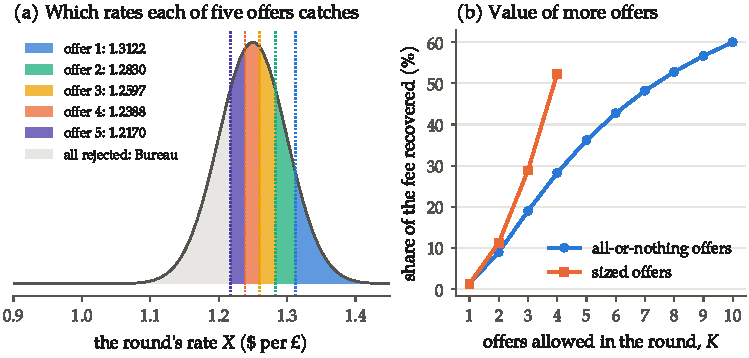
\includegraphics[width=0.72\textwidth]{figures/fig_feedback}
\caption{Several offers in one round, pound seller, $f=\val{p.f}$, no market-maker fee. (a) The optimal five-offer ladder: each offer is made only if the ones before it were rejected, and it fills when the rate lies between it and the previous offer; if all five are rejected the trader uses the Bureau. (b) The value of the round as a share of the fee: all-or-nothing offers (\cref{tab:v1}) and sized offers.}
\label{fig:feedback}
\end{figure}

% =============================================================================
\section{Numerical methods}\label{app:numerics}
% =============================================================================
\paragraph{Grids}
The dynamic programme of \cref{sec:multiround} discretises the offer threshold on \val{grid.noffer} points within $\pm\val{grid.zmax}\,\sigma$ of the anchor (steps of \val{grid.zstep}\,$\sigma$), with \val{grid.quad} quadrature cells per step for the rate, aligned so that the probability of any interval of rates is a table lookup. Holdings of the starting currency use \val{grid.nc} nodes, holdings of the target currency \val{grid.nd} nodes with the target on a node, so that the kink of \eqref{eq:terminal} is represented exactly, and offer sizes \val{grid.nq} fractions of the holding plus two small probes. The anchor uses \val{grid.na} nodes within $\pm\val{grid.ahalf}\,\sigma$ of $a_0$ (steps of \val{grid.astep}\,$\sigma$), with linear interpolation between them; an anchor outside this range, reached by round 4 with probability \val{grid.anchorout}, uses the nearest node's tables, which affects the policy only and leaves every replayed value a valid value of that policy.

\paragraph{The anchor-grid bias}
Linear interpolation overstates a convex function between its nodes by $O(h^2)$ in the node spacing $h$. \Cref{tab:refine} halves the anchor step twice for T1 at $(2\%,0)$ (we did not repeat this at $(2\%,1\%)$): the gap between table and replay falls by factors of \val{refine.ratioa} and \val{refine.ratiob}, and the replayed value does not move. Replayed on the same 20{,}000 paths, the policy from the finest anchor grid gives the same final wealth as the default grid's on \val{gridchk.anchor.same} path. Holdings grids twice as fine ($33\times81$ nodes instead of $17\times41$) give T1 the same final wealth on \val{gridchk.cd.same} path, consistent with its policy: T1 converts everything in round 1, after which its value is piecewise linear in its holdings with the kink on a node. For T2, which carries currency across rounds, the finer holdings grid changes the replayed value by $\val{gridchk.cdB.diff}\pm\val{gridchk.cdB.diffse}$ bp; this test cannot exclude changes of that size, comparable to T2's smaller edges.

\paragraph{Offers outside the threshold grid}
The threshold grid spans $\pm\val{grid.zmax}\,\sigma$ of the anchor, so the dynamic programme cannot make an offer further out; at $(2\%,1\%)$ the dollar seller's best single offer lies $\val{fee.Bz21}\,\sigma$ out. Such offers are worth almost nothing. Take any policy and, whenever it makes an offer outside the grid, replace the offer by no offer and, in the Bureau phase, convert the same amount at the Bureau exactly when the offer would have filled, which the trader can do because the rate is then revealed; everything else is unchanged. The two policies differ only on fills that beat the Bureau, which happen when the rate lands in the fee band next to the threshold, $(1-f)X<P<(1-g)X$ for a pound seller in the notation of \cref{sec:rule}, and its mirror image for a dollar seller. At $(2\%,1\%)$, for any threshold outside the grid and any anchor the programme uses, that band lies far enough out that the round's rate lands in it with probability at most \val{grid.offp}; on such a fill the trader gains at most the fee spread $f-g$ on the amount, scaled by at most $1+\beta$ through the deficit penalty and by the small premium of \cref{prop:siegel}. Under the truncated rate law of \cref{rem:inverse}, over four rounds the replacement loses at most \val{grid.offbound} bp of capital, far below the breakdown threshold of 1 bp.
\begin{table}[!htb]
\centering\small
\begin{threeparttable}
\caption{Refining the anchor grid, T1 at $(2\%,0)$, one offer per round. The replay is floor-anchored on 20{,}000 paths.}
\label{tab:refine}
\begin{tabular}{rrrrr}
\toprule
anchor nodes & step ($\sigma$) & table value & replayed value & table $-$ replay (bp)\\
\midrule
\tablebody{tables/tab_refine.tex}
\bottomrule
\end{tabular}
\end{threeparttable}
\end{table}

\paragraph{The floor-anchored replay}
Replaying the optimal policy on simulated paths estimates its value with the noise of the whole game's P/L. We instead replay it on the same paths as the policy of converting everything at the Bureau in round 1, whose value is known exactly, and report the exact floor plus the mean paired difference. This is a control variate \citep{glasserman2004}: the common noise of the rate path cancels. The verification gate (\cref{app:verification}) replays the policy plainly on 20{,}000 paths, without this cancellation: its table gap for T1 at $(2\%,0)$ is \val{dp.A.f2g0.gap} bp, against \val{dp.A.f2g0.gapfa} for the floor-anchored replay on 200{,}000 paths and \val{refine.gap13} on the 20{,}000 paths of \cref{tab:refine}. The differences are sampling error.

% =============================================================================
\section{Training details}\label{app:training}
% =============================================================================
All training is in double precision. Each trader's network and the market maker's are seeded separately, and training, validation and evaluation games use separate fixed seeds. The ramp width in \eqref{eq:sigmoid} is $\tau$ times the standard deviation of the round's realised rate move in the batch, held fixed in the gradient, and the anneal is geometric.

An earlier design in which the market maker output an acceptance probability collapsed to rejecting everything, where the sigmoid has no gradient. The level of \cref{sec:policies} also starts by rejecting everything, but a level in price units moves through the offers and keeps a gradient. A frozen network's parameters receive no update, but gradients flow through its outputs, so a trader's gradient includes the market maker's response. Each trader's gradient is computed from its own score before any trader's weights move. After each block the agents are scored on 20{,}000 fixed games of the hard game; training stops when the last four outer steps show no paired change larger than two standard errors (or a small fixed tolerance, if that is larger).

The single-trader networks of \cref{sec:validation} are trained for \val{st.iters} iterations of \val{st.batch} games against the flatten-rule market maker, keeping the checkpoint that scores best on a fixed hard-game validation set.

% =============================================================================
\section{Verification}\label{app:verification}
% =============================================================================
\paragraph{Closed form and dynamic programme}
Played through the game's rules on 200{,}000 simulated rounds, the optimal blind offer of \cref{sec:optimal} returns \val{v0.mc} $\pm$ \val{v0.mcse} (two standard errors) dollars per pound, \val{v0.mcgap} standard errors from the closed form; this checks the value, not the much smaller edge, which check (1) below tests. The dynamic programme passes five checks. (1) With one round and no card it reproduces the closed form of \cref{sec:optimal} and the sequential-offer solver of \cref{app:sequential}. (2) With the market maker's fee it reproduces \cref{prop:card}: in one round the fee game equals $(1-g)$ times the $g=0$ game with trader fee $\fp$ solved on the same grid to within \val{gate2.same}, and agrees with the independent sequential-offer solver and the closed form to within \val{gate2.ref}, the grid error of check (1) and well below the breakdown threshold of $10^{-4}$; the whole game on the rescaled card agrees to within \val{gate2.game} of capital. (3) The table value agrees with the plain replay of the policy up to the anchor-grid bias of \cref{app:numerics}. (4) Money is conserved on every replayed path. (5) Every value lies between the Bureau floor and the value of perfect foresight: the expected P/L of a trader who knows the whole rate path, sells to the market maker in the round with the best rate at that rate less the cheaper of the two fees, and chooses how much to sell given its card. This is \val{dp.A.f2g0.cv} for T1 and \val{dp.B.f2g0.cv} for T2 at $(2\%,0)$, against \val{dp.A.f2g0.value} and \val{dp.B.f2g0.value} for optimal play. With the fee setting at zero, the fee-aware solver reproduces the original solver exactly.

\paragraph{Learning runs}
For each of \val{ver.nruns} co-training runs, the market maker's and the traders' books were rebuilt from the recorded games and compared with the recorded values: \val{ver.npassed} pass, with a worst mismatch of \val{ver.worst}. For \val{rep.nruns} runs, \val{rep.nrows} saved training blocks were replayed from their saved weights; the largest difference between saved and replayed P/L is \val{rep.maxgap}.

\paragraph{Reproducibility}
Every number in this paper is a macro written by \texttt{Paper/make\_assets.py}, which computes the model results (closed forms, quadrature and the dynamic programme) from the model code and reads the learning results from the saved runs; \texttt{numbers.json} records, for every number, the function and the file it came from. The same script draws every figure and writes every table body.

% =============================================================================
\section{Robustness}\label{app:robustness}
% =============================================================================
\Cref{tab:robust} repeats the base 2\% co-training with other seeds and settings. Trade survives in every variant but one: when neither agent's acceptance rule is smoothed at the start, the market closes (\cref{sec:equilibria}). Netting is at most \val{rob.maxnetted} of the money in every variant.

\begin{table}[!htb]
\centering\small
\begin{threeparttable}
\caption{The four-trader market at a 2\% spread under other seeds and training settings. Shares of the game's money; P/L in basis points.}
\label{tab:robust}
\begin{tabular}{lrrrrr}
\toprule
run & MM trades & netted & MM to Bureau & all Bureau & MM P/L\\
\midrule
\tablebody{tables/tab_robust.tex}
\bottomrule
\end{tabular}
\end{threeparttable}
\end{table}

% =============================================================================
\section{Learning curves and convergence}\label{app:learning}
% =============================================================================
After each block of co-training the agents are scored on the fixed validation games (\cref{sec:cotrain}). \Cref{tab:learnrange} summarises the last ten blocks of the one-trader runs of \cref{sec:cotrain-results} where the channel is open. \Cref{fig:learning} shows the base four-trader run of \cref{sec:four} block by block, and \cref{tab:learnrange4} summarises its last ten blocks.

\begin{table}[htb]
\centering\small
\begin{threeparttable}
\caption{Does the trader settle? Its edge over the Bureau, in bp of capital, measured after each of the last ten blocks of co-training on the 20{,}000 validation games, where the trading channel is open. A range much wider than the noise of one measurement (two standard errors) means the trader is still moving. The dynamic programme's edge (\cref{tab:feedp}) is for comparison.}
\label{tab:learnrange}
\begin{tabular}{lcrrr}
\toprule
trader, $(f,g)$ & last ten blocks & final & noise & DP edge\\
\midrule
\tablebody{tables/tab_learnrange1.tex}
\bottomrule
\end{tabular}
\end{threeparttable}
\end{table}

\begin{table}[htb]
\centering\small
\begin{threeparttable}
\caption{The four-trader run of \cref{fig:learning} over its last ten blocks: each trader's edge over the Bureau in bp of its capital, and the market maker's P/L in bp of the game's capital, with the noise of one measurement (two standard errors), as in \cref{tab:learnrange}.}
\label{tab:learnrange4}
\begin{tabular}{lcrr}
\toprule
agent & last ten blocks & final & noise\\
\midrule
\tablebody{tables/tab_learnrange4.tex}
\bottomrule
\end{tabular}
\end{threeparttable}
\end{table}

\begin{figure}[p]
\centering
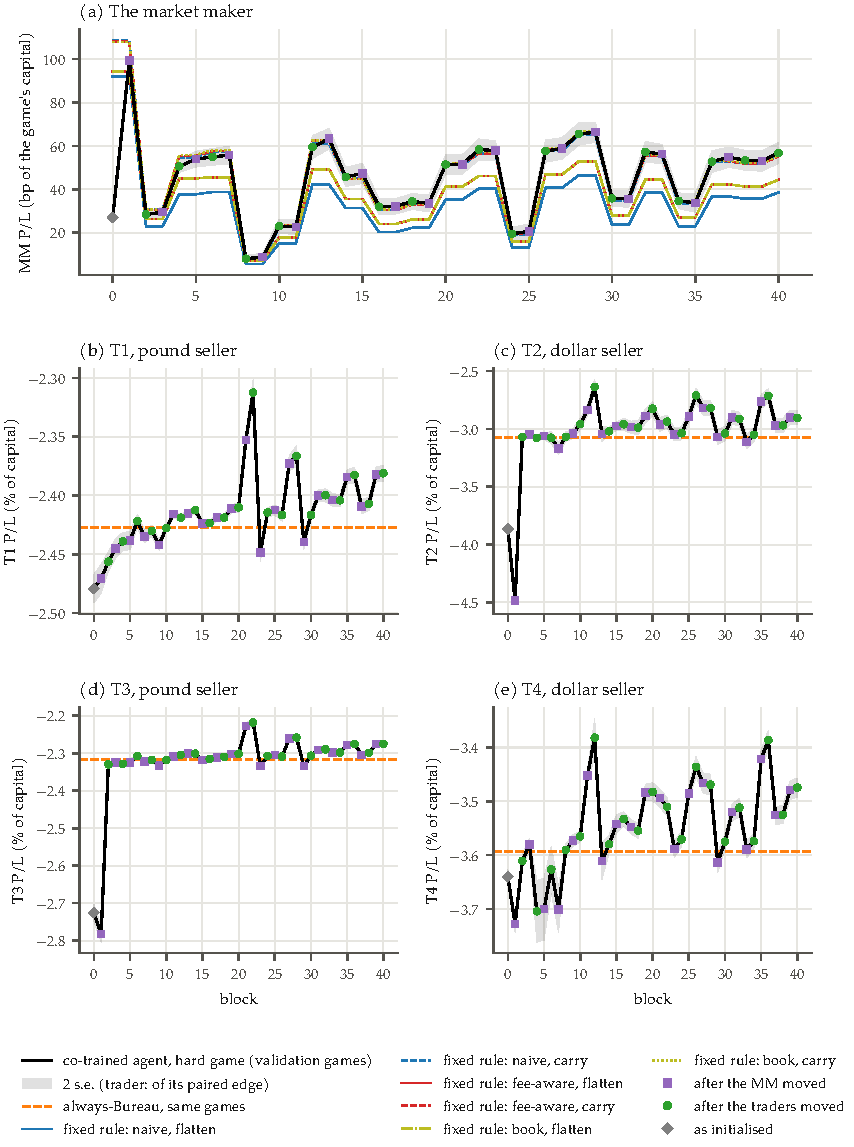
\includegraphics[width=\textwidth]{figures/fig_learning4}
\caption{The four-trader market at a 2\% spread, measured on the fixed validation games after every block of 100 steps; block 0 is the agents as initialised, and markers show who had just moved. (a) The market maker's P/L, with that of each of six fixed rules (naive, fee-aware, or the book rule that tries every subset of the round's offers, each with flatten or carry) against the traders at that block. (b--e) Each trader's P/L, with two standard errors of its edge shaded and, dashed, the P/L of converting everything at the Bureau in round 1 on the same games. Each panel has its own vertical scale.}
\label{fig:learning}
\end{figure}


\end{document}
